%%% -*-LaTeX-*-
%%% ====================================================================
%%% This is a sample top-level LaTeX-2e file for typesetting a thesis
%%% or dissertation at the University of Utah.  Most students find it
%%% convenient to start with a COPY of this file as a template, and
%%% then alter that copy to match their needs.
%%%
%%% There is an associated Unix Makefile that can be similarly
%%% customized, and then the only command ever needed to typeset the
%%% complete thesis is the single word "make".  Of course, during
%%% writing and typesetting, not all of the steps are needed, so
%%% often, one can just name a convenience target such as "make
%%% dvi-pass" or "make pdf-pass" to do just a single pass of LaTeX and
%%% BibTeX.
%%%
%%% There should be no, or very few, macro definitions in this file;
%%% any needed belong in a private style file, called mythesis.sty,
%%% and input below after all other packages.  The bulk of this file
%%% should just be command invocations, and any arguments that they
%%% need.
%%%
%%% We exploit the fact that TeX ignores spaces after command names to
%%% line up arguments for better readability.
%%%
%%% Each chapter should be a separate complete file, so that you can
%%% insert a command like \includeonly{chap_intro} before the first
%%% \include{chap_xxx} command to avoid typesetting all but the
%%% chapter that you are currently working on, to save time.
%%%
%%% Remember that occupants of job positions change jobs from time to
%%% time: YOU are responsible for ensuring correct names of all humans
%%% mentioned in this file!
%%%
%%% [16-Mar-2016]
%%% ====================================================================

\documentclass[11pt,Chicago]{uuthesis2e}

%%% Undefine two macros from uuthesis2e.cls that conflict with
%%% definitions in amsthm.sty that fail to check for prior definitions!
%%% NB: The amsthm package refines the LaTeX theorem environment,
%%% and the uuthesis-color-headings wraps that definition, so the
%%% amsthm package must be read first!
\let \proof    = \relax
\let \endproof = \relax
\usepackage {amsthm}

%%% ====================================================================
%%% Choose an alternate font family for the document if the TeX default
%%% of Computer Modern is not wanted:

\usepackage{mathpazo}

%%% ====================================================================
%%% Some miscellaneous Utah- and student-specific settings:
%%%
%%% Chapter is one level, section and subsection are the next two levels.

\fourlevels

%%% ====================================================================
%%% The remaining packages are required by this particular thesis,
%%% but other theses will almost certainly need different packages:
%%%
%%% WARNING: MANY \LaTeX{} packages change dimensions, glue, and/or
%%% formatting styles, and such changes are likely to conflict with
%%% University of Utah Thesis Office requirements.  Therefore, minimize
%%% the number of packages that you include!

\usepackage{multirow}
\usepackage[table,xcdraw]{xcolor}
\usepackage{amsmath}
\usepackage {amssymb}
\usepackage {bm}
\usepackage {bibnames}
\usepackage {citesort}
\usepackage {graphicx}
\usepackage {graphpap}
\usepackage {longtable}
\usepackage {multirow}
\usepackage {tikz}
\usetikzlibrary {decorations.markings,matrix,positioning}
\usepackage {varioref}

%%% ====================================================================
%%% Support for a subject index:

%% \usepackage {uuthesis-index}

%%% ====================================================================
%%% The various uuthesis-*.sty packages must come AFTER all other
%%% system-provided packages, so that they can correctly override
%%% settings from those packages.

%%% Include latest updates for 2016 (WARNING: the name is subject to
%%% change: see http://www.math.utah.edu/pub/uuthesis/ for the most
%%% current version.)

\usepackage {uuthesis-2016-h}  % MANDATORY package

%%% This is an OPTIONAL package that sets chapter and sectional headings
%%% in color:
%%% Use one or the other of these:
% \usepackage {color}
%%: \usepackage {uuthesis-color-headings}
%%: \definecolor{utahheadingcolor} {rgb}  {0.7, 0.0, 0.0}
%%: \definecolor{utahtheoremcolor} {rgb}  {0.490,0.149,0.804} % purple4
%%: \definecolor{utahtheoremcolor} {rgb}  {0.545,0.137,0.137} % brown4

%%% Here is another, and more convenient, way to define colors, via
%%% aliases of named colors in the X11-derived rgb.sty file

%%: \usepackage{coloralias}
%%: \definecoloralias{utahheadingcolor}{steelblue4}
%%: \definecoloralias{utahtheoremcolor}{hotpink3}

%%% The default heading color is utahred (defined by University Printing
%%% Services as 0.8 red, 0.0 green, 0.0 blue), but you could redefine
%%% that to, for example, a dark blue color, like this AFTER including
%%% the package:
%%%
%%%     \definecolor{utahheading}{rgb}{0,0,0.8}
%%%
%%% NB: Be careful with use of colors in typesetting, and in figures,
%%% because about 6 percent of the human male population is red/green
%%% color blind: they see those colors as shades of brown.  Red and
%%% blue, or blue and green, are better choices for choosing
%%% distinguishable colors.  Also, avoid light colors, especially
%%% yellow, because they are hard to see against white paper and
%%% screen backgrounds, and when printed on black-and-white printers,
%%% where they are rendered in gray, they may be too faint to read.

%%% ====================================================================
%%% Support for a subject index:
%
%: \usepackage {uuthesis-index}

%%% ====================================================================
%%% This single user-specific file is where all personal customizations
%%% and macro definitions should be placed, and it should come LAST,
%%% after ALL OTHER packages, in case it needs to override some of their
%%% definitions.

\usepackage {mythesis}

%%% ====================================================================
%%% The student-specific front matter fields are defined here:

\author                 {Benjamin Richard Draut}
\title                  {SWEETPEA: TOWARD UNIFORM SAMPLING FOR EXPERIMENTAL DESIGN}
\thesistype             {thesis}

\dedication             {For my family}

%%% Most students need just a short degree name, like this:
%\degree                 {Doctor of Philosophy}
%%% However, multiline degrees are possible, and are done like this:
%%% \degree                 {Doctor of Philosophy \\
%%%                         in \\
%%%                         Mathematical Physics}
\degree                 {Master of Science \\
                         in \\
                         Computer Science}

%%% College- and Department-level definitions:
\approvaldepartment     {Computing}
\department             {School of Computing}
\graduatedean           {David B. Kieda}
\departmentchair        {Ross Whitaker}

%%% The graduate student's committee members:
\committeechair         {Matthew Flatt}
\firstreader            {Vivek Srikumar}
\secondreader           {Jonathan Cohen}
\thirdreader            {none}
\fourthreader           {none}
\chairtitle             {Professor}

%%% NB: It is rare, but possible, for there to be two chairs, For
%%% example, one student had
%%%
%%% \committeechair{\mbox{\small Andrej Cherkaev and Andrejs Treibergs}}
%%%
%%% The \mbox{} ensures that line breaks cannot happen, and the \small
%%% is necessary to make the names fit on the Dissertation Approval form

%%% Dates that must be adjusted for each academic term, and be permitted
%%% according to the University of Utah Thesis Office:
\submitdate             {December 2019}
\copyrightyear          {2019}

%%% Dates on which committee members approved the thesis
\chairdateapproved      {22 August 2019}
\firstdateapproved      {22 August 2019}
\seconddateapproved     {08 September 2019}
\thirddateapproved      {none}
\fourthdateapproved     {none}

%%% ====================================================================
%%% Typesetting begins here:

\begin{document}

%% Comment out items by inserting a percent % character
\frontmatterformat
\titlepage
\copyrightpage
\dissertationapproval
\setcounter {page}     {2}             % UofU Thesis Office demands abstract on p. iii: start one lower
\preface    {abstract} {Abstract}
\dedicationpage
\tableofcontents
\listoffigures
\listoftables
%
%%% Optional front matter page(s), made from source "notation.tex". If
%%% you don't need it, then comment out the \optionalfront command
%%% line!  The first argument is the (unnumbered) section header for
%%% the text supplied by the file input by the second argument; that
%%% file must NOT contain \chapter, \section, \subsection, \ldots{}
%%% sectioning commands.

% \optionalfront {Notation and Symbols} {\documentclass[a4paper]{article}

%% Language and font encodings
\usepackage[english]{babel}
\usepackage[utf8x]{inputenc}

\usepackage{booktabs}
\usepackage{tabu}
\usepackage[T1]{fontenc}

%% Sets page size and margins
\usepackage[a4paper,top=3cm,bottom=2cm,left=3cm,right=3cm,marginparwidth=1.75cm]{geometry}

%% Useful packages
\usepackage{amsmath}
\usepackage{graphicx}
%\usepackage{apacite}
\usepackage[colorinlistoftodos]{todonotes}
\usepackage[colorlinks=true, allcolors=blue]{hyperref}

\title{Notation for Solution Counting}
\author{Ben Draut \\ u1066504}
\date{\today}

\begin{document}

\section{Names and Symbols}

A Block contains a set of factors, (design) a set of factors to cross with each other (crossing), and a set of constraints.

Let $D$ be the set of factors in the design. \newline

Let $X$ be the set of factors in the crossing. \newline

Let $C$ be the set of constraints. \newline

Let $\overline{X}$ denote the factors in the design which are \textit{not} in the crossing. \newline

The number of factors/levels in $X$ determines the length of the generated trial sequences, denoted $l$. \newline

Lemmas:

\begin{enumerate}
\item $X \subseteq D$
\item $X \cup \overline{X} = D$
\item $X \cap \overline{X} = \emptyset$
\end{enumerate}

For a given factor $f$, let $|f|$ denote the number of possible settings (levels) for $f$.

\section{Counting Solutions}

\subsection{Simple Factors Only}

This section is limited to designs with only factors that are simple, meaning not derived. (Not dependent on other factors)

So far, this all assumes simple factors, meaning windows with length and stride of 1.
Let $S$ be the set of all valid trial sequences for a given block. We wish to compute $|S|$.

When $C \equiv \emptyset$:

\[
    |S|= {l!}  {\prod_{f \in \overline{X}} {|f|}^l}
\]

Or simply: $l!$ when $\overline{X} \equiv \emptyset$.

\subsubsection{Constraints}

Only two constraints exist right now: \texttt{AtMostKInARow} and \texttt{ExactlyKInARow}. Exactly K is a special case of AtMostK too, so this should resolve to a single formula?

\begin{itemize}
\item \texttt{AtMostKInARow($k$, $f_v$)}
\item \texttt{ExactlyKInARow($k$, $f_v$)}
\end{itemize}

Where $k$ is the integer sequence limit for the level being constrained, and $f_v$ denotes the level $v$ in factor $f$ being constrained.

Each constraint defines an equivalence relation on $S$, which in turn defines a set partition containing two subsets, $A$ and $B$. $A \subseteq S$, while $B \not\subseteq S$.

Let $Q$ be the set of all sets defined by constraints in $C$ to not be in $S$. In otherwords:

\[
    \forall c \in C \text{, } c \to \begin{cases}
      A \mid A \subseteq S\\
      B \mid B \not\subseteq S
    \end{cases}
\]


Then:

\[
    Q = \{{ B_1, B_2, ..., B_i\}}
\]

Where $i = |C|$.

Assuming that all $B_i$, $B_n$ are disjoint:

\[
    |S| = {l!} {\prod_{f \in \overline{X}} {|f|}^l} - \sum_{q \in Q} {|q|}
\]

But how can we count $|B|$?

Because all factors/levels in $X$ are being fully crossed, (this won't be true when specific crossings are excluded) we can compute the number of times $v$ may appear in a sequence, denoted $|v|$.

\[
    |v| = \frac{l}{|f|}
\]

For each sublength $u$ in $(k, |v|]$, how many subsequences of length $s$ can $l$ contain? Denoted $n$. (If $l = 4$ and $u = 2$, then $n = 3$)

It's more like this:

How many unique ways can you arrange $|v|$ items in a sequence of $l$ entries where there is at least one subsequnce that is at least $k$ consecutive elements.

With that, $|B| = nl$. (I think.) So:

\[
    |B| = \sum_{u \in L} ul
\]

Where $L$ is the range $(k, |v|]$.

But it will rarely be this simple, since multiple constraints will almost always overlap, right?

\end{document}}

%%% Uncomment this is you want the contents of acknowledge.tex typeset here.
%%% Note that both "Acknowledgement" and "Acknowledgment" are accepted
%%% spellings of that word.

\preface{acknowledge}{Acknowledgements}

%%% Demonstrations of thesis typesetting features for the sample thesis.
%%% Once you have seen the examples, you can comment out this line.
%%: \optionalfront {Typesetting Experiments} {%%% -*-LaTeX-*-
%%% ====================================================================
%%% This file is intended to be included as a front-matter section of
%%% the sample thesis, with a command like this
%%%
%%% \optionalfront{Typesetting Experiments}{%%% -*-LaTeX-*-
%%% ====================================================================
%%% This file is intended to be included as a front-matter section of
%%% the sample thesis, with a command like this
%%%
%%% \optionalfront{Typesetting Experiments}{%%% -*-LaTeX-*-
%%% ====================================================================
%%% This file is intended to be included as a front-matter section of
%%% the sample thesis, with a command like this
%%%
%%% \optionalfront{Typesetting Experiments}{\input{samples}}
%%%
%%% just before the \maintext macro that begins the body of the thesis,
%%% and starts chapter numbering.
%%%
%%% [16-Mar-2016]
%%% ====================================================================

\input{rgb.sty}

\definecolor{utahred} {rgb} {0.8, 0.0, 0.0} % official definition for University of Utah Printing Services

\doublespace

%% \showthe \baselineskip

In this section, we use color in several places.
The \verb=\colorbox= command takes two arguments
--- a named color and text to be in black on a
background of that color --- and sets the text in
a box with a small margin of width \verb=\fboxsep=
(set to \texttt{\the\fboxsep} in this document).

Here, we want a tighter colored box that has a
fixed height, and is independent of letter shape.
We set the margin to zero inside a group so that
the change is purely local, and so that height and
depth of the line are not increased over what they
would be if the colored box were not used.  We
prefix a \TeX{} \verb=\strut= to the user-supplied
text, because that command expands to a zero-width
box of the height and depth of parentheses, which,
in most fonts, delimit the extent of letter
shapes.

\begin{verbatim}
\newcommand {\hilitebox} [1] {{\fboxsep = 0pt\colorbox{pink}{\strut #1}}}
\end{verbatim}

\newcommand {\hilitebox} [1] {{\fboxsep = 0pt\colorbox{pink}{\strut #1}}}

Here is a fragment from the first chapter in another
thesis, set in \emph{emphasized text} to distinguish it
from the rest of this section:

\begin{itshape}
    In light of the known results, the consistency
    of empirical semivariogram and related
    estimators is widely considered a settled
    matter.  For example, Lahiri, Lee, and Cressie
    \cite{Lahiri:2002:ADA} state:

    \begin{quote}
        The simpler and more commonly used
        nonparametric estimators of the variogram,
        such as the method of moments estimator of
        Matheron (1962) and its robustified
        versions due to Cressie and Hawkins (1980)
        have many desirable properties like,
        unbiasedness, consistency, etc. \ldots
    \end{quote}
    \noindent
    Regarding a kernel estimator of the covariance
    function, Hall and Patil
    \cite{Hall:1994:PNE} remarked:
    \begin{quote}
        It is not difficult to see that if, as $ n
        $ increases, the points $ t_i $ become
        increasingly dense in each bounded subset
        of $ \mathbb{R}^d $, then the bandwidth $
        h $ may be chosen so that $ \check \rho(t)
        \to \rho(t) $ as $ n \to \infty $, for
        each $ t \in \mathbb{R}^d $.
    \end{quote}
    However, in order to be true, such statements
    would need to be qualified by many assumptions
    on the random field as well as on the
    observation locations. We will see in
    \S2.3 that even for well-behaved
    random fields (e.g., $\rho^*$-mixing Gaussian
    random fields), it is not enough to assume
    that the observation locations become
    increasingly dense in each bounded subset; a
    stronger assumption must be made to ensure
    that the observation locations do not become
    denser in one region too much faster than in
    others.
\end{itshape}

The text before the previous paragraph contained
two \texttt{quote} environments separated by a
line of prose.  Here are some more tests of both
kinds of \LaTeX{} environments for showing text
written by someone else.

This is a \hilitebox{\texttt{quote}} environment
with one short line, following a fairly short
paragraph of prose (in this, and following
examples, the text is explicitly colored with a
command like \verb=\color{purple}= inside the
environment before the text):
%
\begin{singlespace}
\color{darkblue}
\begin{verbatim}
\begin{quote}
    \color{purple}
    14 March 2016 is $\pi \approx 3.1416$ day in funny notation.
    \hfill \emph{Web news reports}
\end{quote}
\end{verbatim}
\end{singlespace}
%
\begin{quote}
    \color{purple}
    14 March 2016 is $\pi \approx 3.1416$ day in funny notation.
    \hfill \emph{Web news reports}
\end{quote}

This is a \hilitebox{\texttt{quote}} environment
with three short lines, each a separate paragraph,
following a fairly short paragraph of prose.

\begin{singlespace}
\color{darkblue}
\begin{verbatim}
\begin{quote}
    \color{forestgreen}
    14 March 2016 is $\pi \approx 3.1416$ day in funny notation.
    \hfill \emph{Web news reports}

    14 March 2016 is $\pi \approx 3.1416$ day in funny notation.
    \hfill \emph{Web news reports}

    14 March 2016 is $\pi \approx 3.1416$ day in funny notation.
    \hfill \emph{Web news reports}
\end{quote}
\end{verbatim}
\end{singlespace}
%
\begin{quote}
    \color{forestgreen}
    14 March 2016 is $\pi \approx 3.1416$ day in funny notation.
    \hfill \emph{Web news reports}

    14 March 2016 is $\pi \approx 3.1416$ day in funny notation.
    \hfill \emph{Web news reports}

    14 March 2016 is $\pi \approx 3.1416$ day in funny notation.
    \hfill \emph{Web news reports}
\end{quote}

Here is another example, this time with separate
colors for each paragraph:

\begin{singlespace}
\color{darkblue}
\begin{verbatim}
\begin{quote}
    \color{darkkhaki}
    14 March 2016 is $\pi \approx 3.1416$ day in funny notation.
    \hfill \emph{Web news reports}

    \color{darkmagenta}
    14 March 2016 is $\pi \approx 3.1416$ day in funny notation.
    \hfill \emph{Web news reports}

    \color{darkcyan}
    14 March 2016 is $\pi \approx 3.1416$ day in funny notation.
    \hfill \emph{Web news reports}

    \color{darkorange}
    14 March 2016 is $\pi \approx 3.1416$ day in funny notation.
    14 March 2016 is $\pi \approx 3.1416$ day in funny notation.
    14 March 2016 is $\pi \approx 3.1416$ day in funny notation.
    \linebreak
    \strut
    \hfill \emph{Web news reports}
\end{quote}
\end{verbatim}
\end{singlespace}
%
\begin{quote}
    \color{darkkhaki}
    14 March 2016 is $\pi \approx 3.1416$ day in funny notation.
    \hfill \emph{Web news reports}

    \color{darkmagenta}
    14 March 2016 is $\pi \approx 3.1416$ day in funny notation.
    \hfill \emph{Web news reports}

    \color{darkcyan}
    14 March 2016 is $\pi \approx 3.1416$ day in funny notation.
    \hfill \emph{Web news reports}

    \color{darkorange}
    14 March 2016 is $\pi \approx 3.1416$ day in funny notation.
    14 March 2016 is $\pi \approx 3.1416$ day in funny notation.
    14 March 2016 is $\pi \approx 3.1416$ day in funny notation.
    \linebreak
    \strut
    \hfill \emph{Web news reports}
\end{quote}

Notice that \hilitebox{\texttt{quote}} paragraphs
are \emph{not} indented, but the environment
itself \emph{is} indented on the left and right by
the value of \verb=\leftmargin= (set to
\texttt{\the\leftmargin} in this document, which
should be identical to \verb=2.5em=, where
\verb=1em= = \texttt{\dimen0 = 1em \the\dimen0}).

For debugging purposes, we also have
\verb=\leftmargini= set to
\texttt{\the\leftmargini}, and we have
\verb=\leftmarginii= set to
\texttt{\the\leftmarginii}.

This is a \hilitebox{\texttt{quotation}}
environment with one paragraph, following a fairly
short paragraph of prose (notice that the
\texttt{quotation} paragraphs \emph{are}
indented):

\begin{singlespace}
\color{darkblue}
\begin{verbatim}
\begin{quotation}
    \color{blue}
    Algebra is concerned with manipulation in
    \emph{time}, and geometry is concerned with
    \emph{space}. These are two orthogonal aspects
    of the world, and they represent two different
    points of view in mathematics.  Thus the
    argument or dialogue between mathematicians in
    the past about the relative importance of
    geometry and algebra represents something very
    fundamental.
    \hfill
    \emph{Sir Michael Atiyah}
    % Mathematics in the 20$^{th}$ century
    % NTM {\bf 10}(1--3) 25--39 (September 2002)
    % http://dx.doi.org/10.1007/BF03033096
\end{quotation}
\end{verbatim}
\end{singlespace}
%
\begin{quotation}
    \color{blue}
    Algebra is concerned with manipulation in
    \emph{time}, and geometry is concerned with
    \emph{space}. These are two orthogonal aspects
    of the world, and they represent two different
    points of view in mathematics.  Thus the
    argument or dialogue between mathematicians in
    the past about the relative importance of
    geometry and algebra represents something very
    fundamental.
    \hfill
    \emph{Sir Michael Atiyah}
    % Mathematics in the 20$^{th}$ century
    % NTM {\bf 10}(1--3) 25--39 (September 2002)
    % http://dx.doi.org/10.1007/BF03033096
\end{quotation}

This is a \hilitebox{\texttt{quotation}} environment with three
paragraphs, following a fairly short paragraph of prose:

\begin{quotation}
    \color{utahred}
    Algebra is concerned with manipulation in
    \emph{time}, and geometry is concerned with
    \emph{space}. These are two orthogonal aspects
    of the world, and they represent two different
    points of view in mathematics.  Thus the
    argument or dialogue between mathematicians in
    the past about the relative importance of
    geometry and algebra represents something very
    fundamental.
    \hfill
    \emph{Sir Michael Atiyah}

    Algebra is concerned with manipulation in
    \emph{time}, and geometry is concerned with
    \emph{space}. These are two orthogonal aspects
    of the world, and they represent two different
    points of view in mathematics.  Thus the
    argument or dialogue between mathematicians in
    the past about the relative importance of
    geometry and algebra represents something very
    fundamental.
    \hfill
    \emph{Sir Michael Atiyah}

    Algebra is concerned with manipulation in
    \emph{time}, and geometry is concerned with
    \emph{space}. These are two orthogonal aspects
    of the world, and they represent two different
    points of view in mathematics.  Thus the
    argument or dialogue between mathematicians in
    the past about the relative importance of
    geometry and algebra represents something very
    fundamental.
    \hfill
    \emph{Sir Michael Atiyah}
\end{quotation}

%% \showthe \baselineskip

Now all following text should be back in
double-spaced mode, and just go on and on and on
and on and on and on and on and on and on and on
and on and on and on and on and on and on and on
and on and on and on and on and on and on and on
and on and on and on and on and on and on and on
and on and on and on and on and on and on and on
and on and on and on and on and on and on and on
and on and on and on and on and on and on and on
and on and on and on and on and on and on and on
and on and on and on and on and on and on and on
and on and on and on and on and on and on and on
and on and on and on and on \ldots{}.

%% \showthe \baselineskip

Now all following text should be back in
double-spaced mode, and just go on and on and on
and on and on and on and on and on and on and on
and on and on and on and on and on and on and on
and on and on and on and on and on and on and on
and on and on and on and on and on and on and on
and on and on and on and on and on and on and on
and on and on and on and on and on and on and on
and on and on and on and on and on and on and on
and on and on and on and on and on and on and on
and on and on and on and on and on and on and on
and on and on and on and on and on and on and on
and on and on and on and on \ldots{}.

%%% \showthe \baselineskip
}
%%%
%%% just before the \maintext macro that begins the body of the thesis,
%%% and starts chapter numbering.
%%%
%%% [16-Mar-2016]
%%% ====================================================================

%% Derived from file://ibapah.math.utah.edu/usr/lib/X11/rgb.txt
%% on Wed Jun  9 11:48:18 MDT 2004
%% by ~beebe/src/awk/rgb.awk

\definecolor{aliceblue}{rgb}{0.941,0.973,1}                    	% #f0f8ff 240 248 255 AliceBlue
\definecolor{antiquewhite1}{rgb}{1,0.937,0.859}                	% #ffefdb 255 239 219 AntiqueWhite1
\definecolor{antiquewhite2}{rgb}{0.933,0.875,0.800}            	% #eedfcc 238 223 204 AntiqueWhite2
\definecolor{antiquewhite3}{rgb}{0.804,0.753,0.690}            	% #cdc0b0 205 192 176 AntiqueWhite3
\definecolor{antiquewhite4}{rgb}{0.545,0.514,0.471}            	% #8b8378 139 131 120 AntiqueWhite4
\definecolor{antiquewhite}{rgb}{0.980,0.922,0.843}             	% #faebd7 250 235 215 AntiqueWhite
\definecolor{aquamarine1}{rgb}{0.498,1,0.831}                  	% #7fffd4 127 255 212 aquamarine1
\definecolor{aquamarine2}{rgb}{0.463,0.933,0.776}              	% #76eec6 118 238 198 aquamarine2
\definecolor{aquamarine3}{rgb}{0.400,0.804,0.667}              	% #66cdaa 102 205 170 aquamarine3
\definecolor{aquamarine4}{rgb}{0.271,0.545,0.455}              	% #458b74 69 139 116 aquamarine4
\definecolor{aquamarine}{rgb}{0.498,1,0.831}                   	% #7fffd4 127 255 212 aquamarine
\definecolor{azure1}{rgb}{0.941,1,1}                           	% #f0ffff 240 255 255 azure1
\definecolor{azure2}{rgb}{0.878,0.933,0.933}                   	% #e0eeee 224 238 238 azure2
\definecolor{azure3}{rgb}{0.757,0.804,0.804}                   	% #c1cdcd 193 205 205 azure3
\definecolor{azure4}{rgb}{0.514,0.545,0.545}                   	% #838b8b 131 139 139 azure4
\definecolor{azure}{rgb}{0.941,1,1}                            	% #f0ffff 240 255 255 azure
\definecolor{beige}{rgb}{0.961,0.961,0.863}                    	% #f5f5dc 245 245 220 beige
\definecolor{bisque1}{rgb}{1,0.894,0.769}                      	% #ffe4c4 255 228 196 bisque1
\definecolor{bisque2}{rgb}{0.933,0.835,0.718}                  	% #eed5b7 238 213 183 bisque2
\definecolor{bisque3}{rgb}{0.804,0.718,0.620}                  	% #cdb79e 205 183 158 bisque3
\definecolor{bisque4}{rgb}{0.545,0.490,0.420}                  	% #8b7d6b 139 125 107 bisque4
\definecolor{bisque}{rgb}{1,0.894,0.769}                       	% #ffe4c4 255 228 196 bisque
\definecolor{black}{rgb}{0,0,0}                                	% #000000 0 0 0 black
\definecolor{blanchedalmond}{rgb}{1,0.922,0.804}               	% #ffebcd 255 235 205 BlanchedAlmond
\definecolor{blue1}{rgb}{0,0,1}                                	% #0000ff 0 0 255 blue1
\definecolor{blue2}{rgb}{0,0,0.933}                            	% #0000ee 0 0 238 blue2
\definecolor{blue3}{rgb}{0,0,0.804}                            	% #0000cd 0 0 205 blue3
\definecolor{blue4}{rgb}{0,0,0.545}                            	% #00008b 0 0 139 blue4
\definecolor{blue}{rgb}{0,0,1}                                 	% #0000ff 0 0 255 blue
\definecolor{blueviolet}{rgb}{0.541,0.169,0.886}               	% #8a2be2 138 43 226 BlueViolet
\definecolor{brown1}{rgb}{1,0.251,0.251}                       	% #ff4040 255 64 64 brown1
\definecolor{brown2}{rgb}{0.933,0.231,0.231}                   	% #ee3b3b 238 59 59 brown2
\definecolor{brown3}{rgb}{0.804,0.200,0.200}                   	% #cd3333 205 51 51 brown3
\definecolor{brown4}{rgb}{0.545,0.137,0.137}                   	% #8b2323 139 35 35 brown4
\definecolor{brown}{rgb}{0.647,0.165,0.165}                    	% #a52a2a 165 42 42 brown
\definecolor{burlywood1}{rgb}{1,0.827,0.608}                   	% #ffd39b 255 211 155 burlywood1
\definecolor{burlywood2}{rgb}{0.933,0.773,0.569}               	% #eec591 238 197 145 burlywood2
\definecolor{burlywood3}{rgb}{0.804,0.667,0.490}               	% #cdaa7d 205 170 125 burlywood3
\definecolor{burlywood4}{rgb}{0.545,0.451,0.333}               	% #8b7355 139 115 85 burlywood4
\definecolor{burlywood}{rgb}{0.871,0.722,0.529}                	% #deb887 222 184 135 burlywood
\definecolor{cadetblue1}{rgb}{0.596,0.961,1}                   	% #98f5ff 152 245 255 CadetBlue1
\definecolor{cadetblue2}{rgb}{0.557,0.898,0.933}               	% #8ee5ee 142 229 238 CadetBlue2
\definecolor{cadetblue3}{rgb}{0.478,0.773,0.804}               	% #7ac5cd 122 197 205 CadetBlue3
\definecolor{cadetblue4}{rgb}{0.325,0.525,0.545}               	% #53868b 83 134 139 CadetBlue4
\definecolor{cadetblue}{rgb}{0.373,0.620,0.627}                	% #5f9ea0 95 158 160 CadetBlue
\definecolor{chartreuse1}{rgb}{0.498,1,0}                      	% #7fff00 127 255 0 chartreuse1
\definecolor{chartreuse2}{rgb}{0.463,0.933,0}                  	% #76ee00 118 238 0 chartreuse2
\definecolor{chartreuse3}{rgb}{0.400,0.804,0}                  	% #66cd00 102 205 0 chartreuse3
\definecolor{chartreuse4}{rgb}{0.271,0.545,0}                  	% #458b00 69 139 0 chartreuse4
\definecolor{chartreuse}{rgb}{0.498,1,0}                       	% #7fff00 127 255 0 chartreuse
\definecolor{chocolate1}{rgb}{1,0.498,0.141}                   	% #ff7f24 255 127 36 chocolate1
\definecolor{chocolate2}{rgb}{0.933,0.463,0.129}               	% #ee7621 238 118 33 chocolate2
\definecolor{chocolate3}{rgb}{0.804,0.400,0.114}               	% #cd661d 205 102 29 chocolate3
\definecolor{chocolate4}{rgb}{0.545,0.271,0.075}               	% #8b4513 139 69 19 chocolate4
\definecolor{chocolate}{rgb}{0.824,0.412,0.118}                	% #d2691e 210 105 30 chocolate
\definecolor{coral1}{rgb}{1,0.447,0.337}                       	% #ff7256 255 114 86 coral1
\definecolor{coral2}{rgb}{0.933,0.416,0.314}                   	% #ee6a50 238 106 80 coral2
\definecolor{coral3}{rgb}{0.804,0.357,0.271}                   	% #cd5b45 205 91 69 coral3
\definecolor{coral4}{rgb}{0.545,0.243,0.184}                   	% #8b3e2f 139 62 47 coral4
\definecolor{coral}{rgb}{1,0.498,0.314}                        	% #ff7f50 255 127 80 coral
\definecolor{cornflowerblue}{rgb}{0.392,0.584,0.929}           	% #6495ed 100 149 237 CornflowerBlue
\definecolor{cornsilk1}{rgb}{1,0.973,0.863}                    	% #fff8dc 255 248 220 cornsilk1
\definecolor{cornsilk2}{rgb}{0.933,0.910,0.804}                	% #eee8cd 238 232 205 cornsilk2
\definecolor{cornsilk3}{rgb}{0.804,0.784,0.694}                	% #cdc8b1 205 200 177 cornsilk3
\definecolor{cornsilk4}{rgb}{0.545,0.533,0.471}                	% #8b8878 139 136 120 cornsilk4
\definecolor{cornsilk}{rgb}{1,0.973,0.863}                     	% #fff8dc 255 248 220 cornsilk
\definecolor{cyan1}{rgb}{0,1,1}                                	% #00ffff 0 255 255 cyan1
\definecolor{cyan2}{rgb}{0,0.933,0.933}                        	% #00eeee 0 238 238 cyan2
\definecolor{cyan3}{rgb}{0,0.804,0.804}                        	% #00cdcd 0 205 205 cyan3
\definecolor{cyan4}{rgb}{0,0.545,0.545}                        	% #008b8b 0 139 139 cyan4
\definecolor{cyan}{rgb}{0,1,1}                                 	% #00ffff 0 255 255 cyan
\definecolor{darkblue}{rgb}{0,0,0.545}                         	% #00008b 0 0 139 DarkBlue
\definecolor{darkcyan}{rgb}{0,0.545,0.545}                     	% #008b8b 0 139 139 DarkCyan
\definecolor{darkgoldenrod1}{rgb}{1,0.725,0.059}               	% #ffb90f 255 185 15 DarkGoldenrod1
\definecolor{darkgoldenrod2}{rgb}{0.933,0.678,0.055}           	% #eead0e 238 173 14 DarkGoldenrod2
\definecolor{darkgoldenrod3}{rgb}{0.804,0.584,0.047}           	% #cd950c 205 149 12 DarkGoldenrod3
\definecolor{darkgoldenrod4}{rgb}{0.545,0.396,0.031}           	% #8b6508 139 101 8 DarkGoldenrod4
\definecolor{darkgoldenrod}{rgb}{0.722,0.525,0.043}            	% #b8860b 184 134 11 DarkGoldenrod
\definecolor{darkgray}{rgb}{0.663,0.663,0.663}                 	% #a9a9a9 169 169 169 DarkGray
\definecolor{darkgreen}{rgb}{0,0.392,0}                        	% #006400 0 100 0 DarkGreen
\definecolor{darkgrey}{rgb}{0.663,0.663,0.663}                 	% #a9a9a9 169 169 169 DarkGrey
\definecolor{darkkhaki}{rgb}{0.741,0.718,0.420}                	% #bdb76b 189 183 107 DarkKhaki
\definecolor{darkmagenta}{rgb}{0.545,0,0.545}                  	% #8b008b 139 0 139 DarkMagenta
\definecolor{darkolivegreen1}{rgb}{0.792,1,0.439}              	% #caff70 202 255 112 DarkOliveGreen1
\definecolor{darkolivegreen2}{rgb}{0.737,0.933,0.408}          	% #bcee68 188 238 104 DarkOliveGreen2
\definecolor{darkolivegreen3}{rgb}{0.635,0.804,0.353}          	% #a2cd5a 162 205 90 DarkOliveGreen3
\definecolor{darkolivegreen4}{rgb}{0.431,0.545,0.239}          	% #6e8b3d 110 139 61 DarkOliveGreen4
\definecolor{darkolivegreen}{rgb}{0.333,0.420,0.184}           	% #556b2f 85 107 47 DarkOliveGreen
\definecolor{darkorange1}{rgb}{1,0.498,0}                      	% #ff7f00 255 127 0 DarkOrange1
\definecolor{darkorange2}{rgb}{0.933,0.463,0}                  	% #ee7600 238 118 0 DarkOrange2
\definecolor{darkorange3}{rgb}{0.804,0.400,0}                  	% #cd6600 205 102 0 DarkOrange3
\definecolor{darkorange4}{rgb}{0.545,0.271,0}                  	% #8b4500 139 69 0 DarkOrange4
\definecolor{darkorange}{rgb}{1,0.549,0}                       	% #ff8c00 255 140 0 DarkOrange
\definecolor{darkorchid1}{rgb}{0.749,0.243,1}                  	% #bf3eff 191 62 255 DarkOrchid1
\definecolor{darkorchid2}{rgb}{0.698,0.227,0.933}              	% #b23aee 178 58 238 DarkOrchid2
\definecolor{darkorchid3}{rgb}{0.604,0.196,0.804}              	% #9a32cd 154 50 205 DarkOrchid3
\definecolor{darkorchid4}{rgb}{0.408,0.133,0.545}              	% #68228b 104 34 139 DarkOrchid4
\definecolor{darkorchid}{rgb}{0.600,0.196,0.800}               	% #9932cc 153 50 204 DarkOrchid
\definecolor{darkred}{rgb}{0.545,0,0}                          	% #8b0000 139 0 0 DarkRed
\definecolor{darksalmon}{rgb}{0.914,0.588,0.478}               	% #e9967a 233 150 122 DarkSalmon
\definecolor{darkseagreen1}{rgb}{0.757,1,0.757}                	% #c1ffc1 193 255 193 DarkSeaGreen1
\definecolor{darkseagreen2}{rgb}{0.706,0.933,0.706}            	% #b4eeb4 180 238 180 DarkSeaGreen2
\definecolor{darkseagreen3}{rgb}{0.608,0.804,0.608}            	% #9bcd9b 155 205 155 DarkSeaGreen3
\definecolor{darkseagreen4}{rgb}{0.412,0.545,0.412}            	% #698b69 105 139 105 DarkSeaGreen4
\definecolor{darkseagreen}{rgb}{0.561,0.737,0.561}             	% #8fbc8f 143 188 143 DarkSeaGreen
\definecolor{darkslateblue}{rgb}{0.282,0.239,0.545}            	% #483d8b 72 61 139 DarkSlateBlue
\definecolor{darkslategray1}{rgb}{0.592,1,1}                   	% #97ffff 151 255 255 DarkSlateGray1
\definecolor{darkslategray2}{rgb}{0.553,0.933,0.933}           	% #8deeee 141 238 238 DarkSlateGray2
\definecolor{darkslategray3}{rgb}{0.475,0.804,0.804}           	% #79cdcd 121 205 205 DarkSlateGray3
\definecolor{darkslategray4}{rgb}{0.322,0.545,0.545}           	% #528b8b 82 139 139 DarkSlateGray4
\definecolor{darkslategray}{rgb}{0.184,0.310,0.310}            	% #2f4f4f 47 79 79 DarkSlateGray
\definecolor{darkslategrey}{rgb}{0.184,0.310,0.310}            	% #2f4f4f 47 79 79 DarkSlateGrey
\definecolor{darkturquoise}{rgb}{0,0.808,0.820}                	% #00ced1 0 206 209 DarkTurquoise
\definecolor{darkviolet}{rgb}{0.580,0,0.827}                   	% #9400d3 148 0 211 DarkViolet
\definecolor{deeppink1}{rgb}{1,0.078,0.576}                    	% #ff1493 255 20 147 DeepPink1
\definecolor{deeppink2}{rgb}{0.933,0.071,0.537}                	% #ee1289 238 18 137 DeepPink2
\definecolor{deeppink3}{rgb}{0.804,0.063,0.463}                	% #cd1076 205 16 118 DeepPink3
\definecolor{deeppink4}{rgb}{0.545,0.039,0.314}                	% #8b0a50 139 10 80 DeepPink4
\definecolor{deeppink}{rgb}{1,0.078,0.576}                     	% #ff1493 255 20 147 DeepPink
\definecolor{deepskyblue1}{rgb}{0,0.749,1}                     	% #00bfff 0 191 255 DeepSkyBlue1
\definecolor{deepskyblue2}{rgb}{0,0.698,0.933}                 	% #00b2ee 0 178 238 DeepSkyBlue2
\definecolor{deepskyblue3}{rgb}{0,0.604,0.804}                 	% #009acd 0 154 205 DeepSkyBlue3
\definecolor{deepskyblue4}{rgb}{0,0.408,0.545}                 	% #00688b 0 104 139 DeepSkyBlue4
\definecolor{deepskyblue}{rgb}{0,0.749,1}                      	% #00bfff 0 191 255 DeepSkyBlue
\definecolor{dimgray}{rgb}{0.412,0.412,0.412}                  	% #696969 105 105 105 DimGray
\definecolor{dimgrey}{rgb}{0.412,0.412,0.412}                  	% #696969 105 105 105 DimGrey
\definecolor{dodgerblue1}{rgb}{0.118,0.565,1}                  	% #1e90ff 30 144 255 DodgerBlue1
\definecolor{dodgerblue2}{rgb}{0.110,0.525,0.933}              	% #1c86ee 28 134 238 DodgerBlue2
\definecolor{dodgerblue3}{rgb}{0.094,0.455,0.804}              	% #1874cd 24 116 205 DodgerBlue3
\definecolor{dodgerblue4}{rgb}{0.063,0.306,0.545}              	% #104e8b 16 78 139 DodgerBlue4
\definecolor{dodgerblue}{rgb}{0.118,0.565,1}                   	% #1e90ff 30 144 255 DodgerBlue
\definecolor{firebrick1}{rgb}{1,0.188,0.188}                   	% #ff3030 255 48 48 firebrick1
\definecolor{firebrick2}{rgb}{0.933,0.173,0.173}               	% #ee2c2c 238 44 44 firebrick2
\definecolor{firebrick3}{rgb}{0.804,0.149,0.149}               	% #cd2626 205 38 38 firebrick3
\definecolor{firebrick4}{rgb}{0.545,0.102,0.102}               	% #8b1a1a 139 26 26 firebrick4
\definecolor{firebrick}{rgb}{0.698,0.133,0.133}                	% #b22222 178 34 34 firebrick
\definecolor{floralwhite}{rgb}{1,0.980,0.941}                  	% #fffaf0 255 250 240 FloralWhite
\definecolor{forestgreen}{rgb}{0.133,0.545,0.133}              	% #228b22 34 139 34 ForestGreen
\definecolor{gainsboro}{rgb}{0.863,0.863,0.863}                	% #dcdcdc 220 220 220 gainsboro
\definecolor{ghostwhite}{rgb}{0.973,0.973,1}                   	% #f8f8ff 248 248 255 GhostWhite
\definecolor{gold1}{rgb}{1,0.843,0}                            	% #ffd700 255 215 0 gold1
\definecolor{gold2}{rgb}{0.933,0.788,0}                        	% #eec900 238 201 0 gold2
\definecolor{gold3}{rgb}{0.804,0.678,0}                        	% #cdad00 205 173 0 gold3
\definecolor{gold4}{rgb}{0.545,0.459,0}                        	% #8b7500 139 117 0 gold4
\definecolor{goldenrod1}{rgb}{1,0.757,0.145}                   	% #ffc125 255 193 37 goldenrod1
\definecolor{goldenrod2}{rgb}{0.933,0.706,0.133}               	% #eeb422 238 180 34 goldenrod2
\definecolor{goldenrod3}{rgb}{0.804,0.608,0.114}               	% #cd9b1d 205 155 29 goldenrod3
\definecolor{goldenrod4}{rgb}{0.545,0.412,0.078}               	% #8b6914 139 105 20 goldenrod4
\definecolor{goldenrod}{rgb}{0.855,0.647,0.125}                	% #daa520 218 165 32 goldenrod
\definecolor{gold}{rgb}{1,0.843,0}                             	% #ffd700 255 215 0 gold
\definecolor{gray0}{rgb}{0,0,0}                                	% #000000 0 0 0 gray0
\definecolor{gray100}{rgb}{1,1,1}                              	% #ffffff 255 255 255 gray100
\definecolor{gray10}{rgb}{0.102,0.102,0.102}                   	% #1a1a1a 26 26 26 gray10
\definecolor{gray11}{rgb}{0.110,0.110,0.110}                   	% #1c1c1c 28 28 28 gray11
\definecolor{gray12}{rgb}{0.122,0.122,0.122}                   	% #1f1f1f 31 31 31 gray12
\definecolor{gray13}{rgb}{0.129,0.129,0.129}                   	% #212121 33 33 33 gray13
\definecolor{gray14}{rgb}{0.141,0.141,0.141}                   	% #242424 36 36 36 gray14
\definecolor{gray15}{rgb}{0.149,0.149,0.149}                   	% #262626 38 38 38 gray15
\definecolor{gray16}{rgb}{0.161,0.161,0.161}                   	% #292929 41 41 41 gray16
\definecolor{gray17}{rgb}{0.169,0.169,0.169}                   	% #2b2b2b 43 43 43 gray17
\definecolor{gray18}{rgb}{0.180,0.180,0.180}                   	% #2e2e2e 46 46 46 gray18
\definecolor{gray19}{rgb}{0.188,0.188,0.188}                   	% #303030 48 48 48 gray19
\definecolor{gray1}{rgb}{0.012,0.012,0.012}                    	% #030303 3 3 3 gray1
\definecolor{gray20}{rgb}{0.200,0.200,0.200}                   	% #333333 51 51 51 gray20
\definecolor{gray21}{rgb}{0.212,0.212,0.212}                   	% #363636 54 54 54 gray21
\definecolor{gray22}{rgb}{0.220,0.220,0.220}                   	% #383838 56 56 56 gray22
\definecolor{gray23}{rgb}{0.231,0.231,0.231}                   	% #3b3b3b 59 59 59 gray23
\definecolor{gray24}{rgb}{0.239,0.239,0.239}                   	% #3d3d3d 61 61 61 gray24
\definecolor{gray25}{rgb}{0.251,0.251,0.251}                   	% #404040 64 64 64 gray25
\definecolor{gray26}{rgb}{0.259,0.259,0.259}                   	% #424242 66 66 66 gray26
\definecolor{gray27}{rgb}{0.271,0.271,0.271}                   	% #454545 69 69 69 gray27
\definecolor{gray28}{rgb}{0.278,0.278,0.278}                   	% #474747 71 71 71 gray28
\definecolor{gray29}{rgb}{0.290,0.290,0.290}                   	% #4a4a4a 74 74 74 gray29
\definecolor{gray2}{rgb}{0.020,0.020,0.020}                    	% #050505 5 5 5 gray2
\definecolor{gray30}{rgb}{0.302,0.302,0.302}                   	% #4d4d4d 77 77 77 gray30
\definecolor{gray31}{rgb}{0.310,0.310,0.310}                   	% #4f4f4f 79 79 79 gray31
\definecolor{gray32}{rgb}{0.322,0.322,0.322}                   	% #525252 82 82 82 gray32
\definecolor{gray33}{rgb}{0.329,0.329,0.329}                   	% #545454 84 84 84 gray33
\definecolor{gray34}{rgb}{0.341,0.341,0.341}                   	% #575757 87 87 87 gray34
\definecolor{gray35}{rgb}{0.349,0.349,0.349}                   	% #595959 89 89 89 gray35
\definecolor{gray36}{rgb}{0.361,0.361,0.361}                   	% #5c5c5c 92 92 92 gray36
\definecolor{gray37}{rgb}{0.369,0.369,0.369}                   	% #5e5e5e 94 94 94 gray37
\definecolor{gray38}{rgb}{0.380,0.380,0.380}                   	% #616161 97 97 97 gray38
\definecolor{gray39}{rgb}{0.388,0.388,0.388}                   	% #636363 99 99 99 gray39
\definecolor{gray3}{rgb}{0.031,0.031,0.031}                    	% #080808 8 8 8 gray3
\definecolor{gray40}{rgb}{0.400,0.400,0.400}                   	% #666666 102 102 102 gray40
\definecolor{gray41}{rgb}{0.412,0.412,0.412}                   	% #696969 105 105 105 gray41
\definecolor{gray42}{rgb}{0.420,0.420,0.420}                   	% #6b6b6b 107 107 107 gray42
\definecolor{gray43}{rgb}{0.431,0.431,0.431}                   	% #6e6e6e 110 110 110 gray43
\definecolor{gray44}{rgb}{0.439,0.439,0.439}                   	% #707070 112 112 112 gray44
\definecolor{gray45}{rgb}{0.451,0.451,0.451}                   	% #737373 115 115 115 gray45
\definecolor{gray46}{rgb}{0.459,0.459,0.459}                   	% #757575 117 117 117 gray46
\definecolor{gray47}{rgb}{0.471,0.471,0.471}                   	% #787878 120 120 120 gray47
\definecolor{gray48}{rgb}{0.478,0.478,0.478}                   	% #7a7a7a 122 122 122 gray48
\definecolor{gray49}{rgb}{0.490,0.490,0.490}                   	% #7d7d7d 125 125 125 gray49
\definecolor{gray4}{rgb}{0.039,0.039,0.039}                    	% #0a0a0a 10 10 10 gray4
\definecolor{gray50}{rgb}{0.498,0.498,0.498}                   	% #7f7f7f 127 127 127 gray50
\definecolor{gray51}{rgb}{0.510,0.510,0.510}                   	% #828282 130 130 130 gray51
\definecolor{gray52}{rgb}{0.522,0.522,0.522}                   	% #858585 133 133 133 gray52
\definecolor{gray53}{rgb}{0.529,0.529,0.529}                   	% #878787 135 135 135 gray53
\definecolor{gray54}{rgb}{0.541,0.541,0.541}                   	% #8a8a8a 138 138 138 gray54
\definecolor{gray55}{rgb}{0.549,0.549,0.549}                   	% #8c8c8c 140 140 140 gray55
\definecolor{gray56}{rgb}{0.561,0.561,0.561}                   	% #8f8f8f 143 143 143 gray56
\definecolor{gray57}{rgb}{0.569,0.569,0.569}                   	% #919191 145 145 145 gray57
\definecolor{gray58}{rgb}{0.580,0.580,0.580}                   	% #949494 148 148 148 gray58
\definecolor{gray59}{rgb}{0.588,0.588,0.588}                   	% #969696 150 150 150 gray59
\definecolor{gray5}{rgb}{0.051,0.051,0.051}                    	% #0d0d0d 13 13 13 gray5
\definecolor{gray60}{rgb}{0.600,0.600,0.600}                   	% #999999 153 153 153 gray60
\definecolor{gray61}{rgb}{0.612,0.612,0.612}                   	% #9c9c9c 156 156 156 gray61
\definecolor{gray62}{rgb}{0.620,0.620,0.620}                   	% #9e9e9e 158 158 158 gray62
\definecolor{gray63}{rgb}{0.631,0.631,0.631}                   	% #a1a1a1 161 161 161 gray63
\definecolor{gray64}{rgb}{0.639,0.639,0.639}                   	% #a3a3a3 163 163 163 gray64
\definecolor{gray65}{rgb}{0.651,0.651,0.651}                   	% #a6a6a6 166 166 166 gray65
\definecolor{gray66}{rgb}{0.659,0.659,0.659}                   	% #a8a8a8 168 168 168 gray66
\definecolor{gray67}{rgb}{0.671,0.671,0.671}                   	% #ababab 171 171 171 gray67
\definecolor{gray68}{rgb}{0.678,0.678,0.678}                   	% #adadad 173 173 173 gray68
\definecolor{gray69}{rgb}{0.690,0.690,0.690}                   	% #b0b0b0 176 176 176 gray69
\definecolor{gray6}{rgb}{0.059,0.059,0.059}                    	% #0f0f0f 15 15 15 gray6
\definecolor{gray70}{rgb}{0.702,0.702,0.702}                   	% #b3b3b3 179 179 179 gray70
\definecolor{gray71}{rgb}{0.710,0.710,0.710}                   	% #b5b5b5 181 181 181 gray71
\definecolor{gray72}{rgb}{0.722,0.722,0.722}                   	% #b8b8b8 184 184 184 gray72
\definecolor{gray73}{rgb}{0.729,0.729,0.729}                   	% #bababa 186 186 186 gray73
\definecolor{gray74}{rgb}{0.741,0.741,0.741}                   	% #bdbdbd 189 189 189 gray74
\definecolor{gray75}{rgb}{0.749,0.749,0.749}                   	% #bfbfbf 191 191 191 gray75
\definecolor{gray76}{rgb}{0.761,0.761,0.761}                   	% #c2c2c2 194 194 194 gray76
\definecolor{gray77}{rgb}{0.769,0.769,0.769}                   	% #c4c4c4 196 196 196 gray77
\definecolor{gray78}{rgb}{0.780,0.780,0.780}                   	% #c7c7c7 199 199 199 gray78
\definecolor{gray79}{rgb}{0.788,0.788,0.788}                   	% #c9c9c9 201 201 201 gray79
\definecolor{gray7}{rgb}{0.071,0.071,0.071}                    	% #121212 18 18 18 gray7
\definecolor{gray80}{rgb}{0.800,0.800,0.800}                   	% #cccccc 204 204 204 gray80
\definecolor{gray81}{rgb}{0.812,0.812,0.812}                   	% #cfcfcf 207 207 207 gray81
\definecolor{gray82}{rgb}{0.820,0.820,0.820}                   	% #d1d1d1 209 209 209 gray82
\definecolor{gray83}{rgb}{0.831,0.831,0.831}                   	% #d4d4d4 212 212 212 gray83
\definecolor{gray84}{rgb}{0.839,0.839,0.839}                   	% #d6d6d6 214 214 214 gray84
\definecolor{gray85}{rgb}{0.851,0.851,0.851}                   	% #d9d9d9 217 217 217 gray85
\definecolor{gray86}{rgb}{0.859,0.859,0.859}                   	% #dbdbdb 219 219 219 gray86
\definecolor{gray87}{rgb}{0.871,0.871,0.871}                   	% #dedede 222 222 222 gray87
\definecolor{gray88}{rgb}{0.878,0.878,0.878}                   	% #e0e0e0 224 224 224 gray88
\definecolor{gray89}{rgb}{0.890,0.890,0.890}                   	% #e3e3e3 227 227 227 gray89
\definecolor{gray8}{rgb}{0.078,0.078,0.078}                    	% #141414 20 20 20 gray8
\definecolor{gray90}{rgb}{0.898,0.898,0.898}                   	% #e5e5e5 229 229 229 gray90
\definecolor{gray91}{rgb}{0.910,0.910,0.910}                   	% #e8e8e8 232 232 232 gray91
\definecolor{gray92}{rgb}{0.922,0.922,0.922}                   	% #ebebeb 235 235 235 gray92
\definecolor{gray93}{rgb}{0.929,0.929,0.929}                   	% #ededed 237 237 237 gray93
\definecolor{gray94}{rgb}{0.941,0.941,0.941}                   	% #f0f0f0 240 240 240 gray94
\definecolor{gray95}{rgb}{0.949,0.949,0.949}                   	% #f2f2f2 242 242 242 gray95
\definecolor{gray96}{rgb}{0.961,0.961,0.961}                   	% #f5f5f5 245 245 245 gray96
\definecolor{gray97}{rgb}{0.969,0.969,0.969}                   	% #f7f7f7 247 247 247 gray97
\definecolor{gray98}{rgb}{0.980,0.980,0.980}                   	% #fafafa 250 250 250 gray98
\definecolor{gray99}{rgb}{0.988,0.988,0.988}                   	% #fcfcfc 252 252 252 gray99
\definecolor{gray9}{rgb}{0.090,0.090,0.090}                    	% #171717 23 23 23 gray9
\definecolor{gray}{rgb}{0.745,0.745,0.745}                     	% #bebebe 190 190 190 gray
\definecolor{green1}{rgb}{0,1,0}                               	% #00ff00 0 255 0 green1
\definecolor{green2}{rgb}{0,0.933,0}                           	% #00ee00 0 238 0 green2
\definecolor{green3}{rgb}{0,0.804,0}                           	% #00cd00 0 205 0 green3
\definecolor{green4}{rgb}{0,0.545,0}                           	% #008b00 0 139 0 green4
\definecolor{green}{rgb}{0,1,0}                                	% #00ff00 0 255 0 green
\definecolor{greenyellow}{rgb}{0.678,1,0.184}                  	% #adff2f 173 255 47 GreenYellow
\definecolor{grey0}{rgb}{0,0,0}                                	% #000000 0 0 0 grey0
\definecolor{grey100}{rgb}{1,1,1}                              	% #ffffff 255 255 255 grey100
\definecolor{grey10}{rgb}{0.102,0.102,0.102}                   	% #1a1a1a 26 26 26 grey10
\definecolor{grey11}{rgb}{0.110,0.110,0.110}                   	% #1c1c1c 28 28 28 grey11
\definecolor{grey12}{rgb}{0.122,0.122,0.122}                   	% #1f1f1f 31 31 31 grey12
\definecolor{grey13}{rgb}{0.129,0.129,0.129}                   	% #212121 33 33 33 grey13
\definecolor{grey14}{rgb}{0.141,0.141,0.141}                   	% #242424 36 36 36 grey14
\definecolor{grey15}{rgb}{0.149,0.149,0.149}                   	% #262626 38 38 38 grey15
\definecolor{grey16}{rgb}{0.161,0.161,0.161}                   	% #292929 41 41 41 grey16
\definecolor{grey17}{rgb}{0.169,0.169,0.169}                   	% #2b2b2b 43 43 43 grey17
\definecolor{grey18}{rgb}{0.180,0.180,0.180}                   	% #2e2e2e 46 46 46 grey18
\definecolor{grey19}{rgb}{0.188,0.188,0.188}                   	% #303030 48 48 48 grey19
\definecolor{grey1}{rgb}{0.012,0.012,0.012}                    	% #030303 3 3 3 grey1
\definecolor{grey20}{rgb}{0.200,0.200,0.200}                   	% #333333 51 51 51 grey20
\definecolor{grey21}{rgb}{0.212,0.212,0.212}                   	% #363636 54 54 54 grey21
\definecolor{grey22}{rgb}{0.220,0.220,0.220}                   	% #383838 56 56 56 grey22
\definecolor{grey23}{rgb}{0.231,0.231,0.231}                   	% #3b3b3b 59 59 59 grey23
\definecolor{grey24}{rgb}{0.239,0.239,0.239}                   	% #3d3d3d 61 61 61 grey24
\definecolor{grey25}{rgb}{0.251,0.251,0.251}                   	% #404040 64 64 64 grey25
\definecolor{grey26}{rgb}{0.259,0.259,0.259}                   	% #424242 66 66 66 grey26
\definecolor{grey27}{rgb}{0.271,0.271,0.271}                   	% #454545 69 69 69 grey27
\definecolor{grey28}{rgb}{0.278,0.278,0.278}                   	% #474747 71 71 71 grey28
\definecolor{grey29}{rgb}{0.290,0.290,0.290}                   	% #4a4a4a 74 74 74 grey29
\definecolor{grey2}{rgb}{0.020,0.020,0.020}                    	% #050505 5 5 5 grey2
\definecolor{grey30}{rgb}{0.302,0.302,0.302}                   	% #4d4d4d 77 77 77 grey30
\definecolor{grey31}{rgb}{0.310,0.310,0.310}                   	% #4f4f4f 79 79 79 grey31
\definecolor{grey32}{rgb}{0.322,0.322,0.322}                   	% #525252 82 82 82 grey32
\definecolor{grey33}{rgb}{0.329,0.329,0.329}                   	% #545454 84 84 84 grey33
\definecolor{grey34}{rgb}{0.341,0.341,0.341}                   	% #575757 87 87 87 grey34
\definecolor{grey35}{rgb}{0.349,0.349,0.349}                   	% #595959 89 89 89 grey35
\definecolor{grey36}{rgb}{0.361,0.361,0.361}                   	% #5c5c5c 92 92 92 grey36
\definecolor{grey37}{rgb}{0.369,0.369,0.369}                   	% #5e5e5e 94 94 94 grey37
\definecolor{grey38}{rgb}{0.380,0.380,0.380}                   	% #616161 97 97 97 grey38
\definecolor{grey39}{rgb}{0.388,0.388,0.388}                   	% #636363 99 99 99 grey39
\definecolor{grey3}{rgb}{0.031,0.031,0.031}                    	% #080808 8 8 8 grey3
\definecolor{grey40}{rgb}{0.400,0.400,0.400}                   	% #666666 102 102 102 grey40
\definecolor{grey41}{rgb}{0.412,0.412,0.412}                   	% #696969 105 105 105 grey41
\definecolor{grey42}{rgb}{0.420,0.420,0.420}                   	% #6b6b6b 107 107 107 grey42
\definecolor{grey43}{rgb}{0.431,0.431,0.431}                   	% #6e6e6e 110 110 110 grey43
\definecolor{grey44}{rgb}{0.439,0.439,0.439}                   	% #707070 112 112 112 grey44
\definecolor{grey45}{rgb}{0.451,0.451,0.451}                   	% #737373 115 115 115 grey45
\definecolor{grey46}{rgb}{0.459,0.459,0.459}                   	% #757575 117 117 117 grey46
\definecolor{grey47}{rgb}{0.471,0.471,0.471}                   	% #787878 120 120 120 grey47
\definecolor{grey48}{rgb}{0.478,0.478,0.478}                   	% #7a7a7a 122 122 122 grey48
\definecolor{grey49}{rgb}{0.490,0.490,0.490}                   	% #7d7d7d 125 125 125 grey49
\definecolor{grey4}{rgb}{0.039,0.039,0.039}                    	% #0a0a0a 10 10 10 grey4
\definecolor{grey50}{rgb}{0.498,0.498,0.498}                   	% #7f7f7f 127 127 127 grey50
\definecolor{grey51}{rgb}{0.510,0.510,0.510}                   	% #828282 130 130 130 grey51
\definecolor{grey52}{rgb}{0.522,0.522,0.522}                   	% #858585 133 133 133 grey52
\definecolor{grey53}{rgb}{0.529,0.529,0.529}                   	% #878787 135 135 135 grey53
\definecolor{grey54}{rgb}{0.541,0.541,0.541}                   	% #8a8a8a 138 138 138 grey54
\definecolor{grey55}{rgb}{0.549,0.549,0.549}                   	% #8c8c8c 140 140 140 grey55
\definecolor{grey56}{rgb}{0.561,0.561,0.561}                   	% #8f8f8f 143 143 143 grey56
\definecolor{grey57}{rgb}{0.569,0.569,0.569}                   	% #919191 145 145 145 grey57
\definecolor{grey58}{rgb}{0.580,0.580,0.580}                   	% #949494 148 148 148 grey58
\definecolor{grey59}{rgb}{0.588,0.588,0.588}                   	% #969696 150 150 150 grey59
\definecolor{grey5}{rgb}{0.051,0.051,0.051}                    	% #0d0d0d 13 13 13 grey5
\definecolor{grey60}{rgb}{0.600,0.600,0.600}                   	% #999999 153 153 153 grey60
\definecolor{grey61}{rgb}{0.612,0.612,0.612}                   	% #9c9c9c 156 156 156 grey61
\definecolor{grey62}{rgb}{0.620,0.620,0.620}                   	% #9e9e9e 158 158 158 grey62
\definecolor{grey63}{rgb}{0.631,0.631,0.631}                   	% #a1a1a1 161 161 161 grey63
\definecolor{grey64}{rgb}{0.639,0.639,0.639}                   	% #a3a3a3 163 163 163 grey64
\definecolor{grey65}{rgb}{0.651,0.651,0.651}                   	% #a6a6a6 166 166 166 grey65
\definecolor{grey66}{rgb}{0.659,0.659,0.659}                   	% #a8a8a8 168 168 168 grey66
\definecolor{grey67}{rgb}{0.671,0.671,0.671}                   	% #ababab 171 171 171 grey67
\definecolor{grey68}{rgb}{0.678,0.678,0.678}                   	% #adadad 173 173 173 grey68
\definecolor{grey69}{rgb}{0.690,0.690,0.690}                   	% #b0b0b0 176 176 176 grey69
\definecolor{grey6}{rgb}{0.059,0.059,0.059}                    	% #0f0f0f 15 15 15 grey6
\definecolor{grey70}{rgb}{0.702,0.702,0.702}                   	% #b3b3b3 179 179 179 grey70
\definecolor{grey71}{rgb}{0.710,0.710,0.710}                   	% #b5b5b5 181 181 181 grey71
\definecolor{grey72}{rgb}{0.722,0.722,0.722}                   	% #b8b8b8 184 184 184 grey72
\definecolor{grey73}{rgb}{0.729,0.729,0.729}                   	% #bababa 186 186 186 grey73
\definecolor{grey74}{rgb}{0.741,0.741,0.741}                   	% #bdbdbd 189 189 189 grey74
\definecolor{grey75}{rgb}{0.749,0.749,0.749}                   	% #bfbfbf 191 191 191 grey75
\definecolor{grey76}{rgb}{0.761,0.761,0.761}                   	% #c2c2c2 194 194 194 grey76
\definecolor{grey77}{rgb}{0.769,0.769,0.769}                   	% #c4c4c4 196 196 196 grey77
\definecolor{grey78}{rgb}{0.780,0.780,0.780}                   	% #c7c7c7 199 199 199 grey78
\definecolor{grey79}{rgb}{0.788,0.788,0.788}                   	% #c9c9c9 201 201 201 grey79
\definecolor{grey7}{rgb}{0.071,0.071,0.071}                    	% #121212 18 18 18 grey7
\definecolor{grey80}{rgb}{0.800,0.800,0.800}                   	% #cccccc 204 204 204 grey80
\definecolor{grey81}{rgb}{0.812,0.812,0.812}                   	% #cfcfcf 207 207 207 grey81
\definecolor{grey82}{rgb}{0.820,0.820,0.820}                   	% #d1d1d1 209 209 209 grey82
\definecolor{grey83}{rgb}{0.831,0.831,0.831}                   	% #d4d4d4 212 212 212 grey83
\definecolor{grey84}{rgb}{0.839,0.839,0.839}                   	% #d6d6d6 214 214 214 grey84
\definecolor{grey85}{rgb}{0.851,0.851,0.851}                   	% #d9d9d9 217 217 217 grey85
\definecolor{grey86}{rgb}{0.859,0.859,0.859}                   	% #dbdbdb 219 219 219 grey86
\definecolor{grey87}{rgb}{0.871,0.871,0.871}                   	% #dedede 222 222 222 grey87
\definecolor{grey88}{rgb}{0.878,0.878,0.878}                   	% #e0e0e0 224 224 224 grey88
\definecolor{grey89}{rgb}{0.890,0.890,0.890}                   	% #e3e3e3 227 227 227 grey89
\definecolor{grey8}{rgb}{0.078,0.078,0.078}                    	% #141414 20 20 20 grey8
\definecolor{grey90}{rgb}{0.898,0.898,0.898}                   	% #e5e5e5 229 229 229 grey90
\definecolor{grey91}{rgb}{0.910,0.910,0.910}                   	% #e8e8e8 232 232 232 grey91
\definecolor{grey92}{rgb}{0.922,0.922,0.922}                   	% #ebebeb 235 235 235 grey92
\definecolor{grey93}{rgb}{0.929,0.929,0.929}                   	% #ededed 237 237 237 grey93
\definecolor{grey94}{rgb}{0.941,0.941,0.941}                   	% #f0f0f0 240 240 240 grey94
\definecolor{grey95}{rgb}{0.949,0.949,0.949}                   	% #f2f2f2 242 242 242 grey95
\definecolor{grey96}{rgb}{0.961,0.961,0.961}                   	% #f5f5f5 245 245 245 grey96
\definecolor{grey97}{rgb}{0.969,0.969,0.969}                   	% #f7f7f7 247 247 247 grey97
\definecolor{grey98}{rgb}{0.980,0.980,0.980}                   	% #fafafa 250 250 250 grey98
\definecolor{grey99}{rgb}{0.988,0.988,0.988}                   	% #fcfcfc 252 252 252 grey99
\definecolor{grey9}{rgb}{0.090,0.090,0.090}                    	% #171717 23 23 23 grey9
\definecolor{grey}{rgb}{0.745,0.745,0.745}                     	% #bebebe 190 190 190 grey
\definecolor{honeydew1}{rgb}{0.941,1,0.941}                    	% #f0fff0 240 255 240 honeydew1
\definecolor{honeydew2}{rgb}{0.878,0.933,0.878}                	% #e0eee0 224 238 224 honeydew2
\definecolor{honeydew3}{rgb}{0.757,0.804,0.757}                	% #c1cdc1 193 205 193 honeydew3
\definecolor{honeydew4}{rgb}{0.514,0.545,0.514}                	% #838b83 131 139 131 honeydew4
\definecolor{honeydew}{rgb}{0.941,1,0.941}                     	% #f0fff0 240 255 240 honeydew
\definecolor{hotpink1}{rgb}{1,0.431,0.706}                     	% #ff6eb4 255 110 180 HotPink1
\definecolor{hotpink2}{rgb}{0.933,0.416,0.655}                 	% #ee6aa7 238 106 167 HotPink2
\definecolor{hotpink3}{rgb}{0.804,0.376,0.565}                 	% #cd6090 205 96 144 HotPink3
\definecolor{hotpink4}{rgb}{0.545,0.227,0.384}                 	% #8b3a62 139 58 98 HotPink4
\definecolor{hotpink}{rgb}{1,0.412,0.706}                      	% #ff69b4 255 105 180 HotPink
\definecolor{indianred1}{rgb}{1,0.416,0.416}                   	% #ff6a6a 255 106 106 IndianRed1
\definecolor{indianred2}{rgb}{0.933,0.388,0.388}               	% #ee6363 238 99 99 IndianRed2
\definecolor{indianred3}{rgb}{0.804,0.333,0.333}               	% #cd5555 205 85 85 IndianRed3
\definecolor{indianred4}{rgb}{0.545,0.227,0.227}               	% #8b3a3a 139 58 58 IndianRed4
\definecolor{indianred}{rgb}{0.804,0.361,0.361}                	% #cd5c5c 205 92 92 IndianRed
\definecolor{ivory1}{rgb}{1,1,0.941}                           	% #fffff0 255 255 240 ivory1
\definecolor{ivory2}{rgb}{0.933,0.933,0.878}                   	% #eeeee0 238 238 224 ivory2
\definecolor{ivory3}{rgb}{0.804,0.804,0.757}                   	% #cdcdc1 205 205 193 ivory3
\definecolor{ivory4}{rgb}{0.545,0.545,0.514}                   	% #8b8b83 139 139 131 ivory4
\definecolor{ivory}{rgb}{1,1,0.941}                            	% #fffff0 255 255 240 ivory
\definecolor{khaki1}{rgb}{1,0.965,0.561}                       	% #fff68f 255 246 143 khaki1
\definecolor{khaki2}{rgb}{0.933,0.902,0.522}                   	% #eee685 238 230 133 khaki2
\definecolor{khaki3}{rgb}{0.804,0.776,0.451}                   	% #cdc673 205 198 115 khaki3
\definecolor{khaki4}{rgb}{0.545,0.525,0.306}                   	% #8b864e 139 134 78 khaki4
\definecolor{khaki}{rgb}{0.941,0.902,0.549}                    	% #f0e68c 240 230 140 khaki
\definecolor{lavenderblush1}{rgb}{1,0.941,0.961}               	% #fff0f5 255 240 245 LavenderBlush1
\definecolor{lavenderblush2}{rgb}{0.933,0.878,0.898}           	% #eee0e5 238 224 229 LavenderBlush2
\definecolor{lavenderblush3}{rgb}{0.804,0.757,0.773}           	% #cdc1c5 205 193 197 LavenderBlush3
\definecolor{lavenderblush4}{rgb}{0.545,0.514,0.525}           	% #8b8386 139 131 134 LavenderBlush4
\definecolor{lavenderblush}{rgb}{1,0.941,0.961}                	% #fff0f5 255 240 245 LavenderBlush
\definecolor{lavender}{rgb}{0.902,0.902,0.980}                 	% #e6e6fa 230 230 250 lavender
\definecolor{lawngreen}{rgb}{0.486,0.988,0}                    	% #7cfc00 124 252 0 LawnGreen
\definecolor{lemonchiffon1}{rgb}{1,0.980,0.804}                	% #fffacd 255 250 205 LemonChiffon1
\definecolor{lemonchiffon2}{rgb}{0.933,0.914,0.749}            	% #eee9bf 238 233 191 LemonChiffon2
\definecolor{lemonchiffon3}{rgb}{0.804,0.788,0.647}            	% #cdc9a5 205 201 165 LemonChiffon3
\definecolor{lemonchiffon4}{rgb}{0.545,0.537,0.439}            	% #8b8970 139 137 112 LemonChiffon4
\definecolor{lemonchiffon}{rgb}{1,0.980,0.804}                 	% #fffacd 255 250 205 LemonChiffon
\definecolor{lightblue1}{rgb}{0.749,0.937,1}                   	% #bfefff 191 239 255 LightBlue1
\definecolor{lightblue2}{rgb}{0.698,0.875,0.933}               	% #b2dfee 178 223 238 LightBlue2
\definecolor{lightblue3}{rgb}{0.604,0.753,0.804}               	% #9ac0cd 154 192 205 LightBlue3
\definecolor{lightblue4}{rgb}{0.408,0.514,0.545}               	% #68838b 104 131 139 LightBlue4
\definecolor{lightblue}{rgb}{0.678,0.847,0.902}                	% #add8e6 173 216 230 LightBlue
\definecolor{lightcoral}{rgb}{0.941,0.502,0.502}               	% #f08080 240 128 128 LightCoral
\definecolor{lightcyan1}{rgb}{0.878,1,1}                       	% #e0ffff 224 255 255 LightCyan1
\definecolor{lightcyan2}{rgb}{0.820,0.933,0.933}               	% #d1eeee 209 238 238 LightCyan2
\definecolor{lightcyan3}{rgb}{0.706,0.804,0.804}               	% #b4cdcd 180 205 205 LightCyan3
\definecolor{lightcyan4}{rgb}{0.478,0.545,0.545}               	% #7a8b8b 122 139 139 LightCyan4
\definecolor{lightcyan}{rgb}{0.878,1,1}                        	% #e0ffff 224 255 255 LightCyan
\definecolor{lightgoldenrod1}{rgb}{1,0.925,0.545}              	% #ffec8b 255 236 139 LightGoldenrod1
\definecolor{lightgoldenrod2}{rgb}{0.933,0.863,0.510}          	% #eedc82 238 220 130 LightGoldenrod2
\definecolor{lightgoldenrod3}{rgb}{0.804,0.745,0.439}          	% #cdbe70 205 190 112 LightGoldenrod3
\definecolor{lightgoldenrod4}{rgb}{0.545,0.506,0.298}          	% #8b814c 139 129 76 LightGoldenrod4
\definecolor{lightgoldenrod}{rgb}{0.933,0.867,0.510}           	% #eedd82 238 221 130 LightGoldenrod
\definecolor{lightgoldenrodyellow}{rgb}{0.980,0.980,0.824}     	% #fafad2 250 250 210 LightGoldenrodYellow
\definecolor{lightgray}{rgb}{0.827,0.827,0.827}                	% #d3d3d3 211 211 211 LightGray
\definecolor{lightgreen}{rgb}{0.565,0.933,0.565}               	% #90ee90 144 238 144 LightGreen
\definecolor{lightgrey}{rgb}{0.827,0.827,0.827}                	% #d3d3d3 211 211 211 LightGrey
\definecolor{lightpink1}{rgb}{1,0.682,0.725}                   	% #ffaeb9 255 174 185 LightPink1
\definecolor{lightpink2}{rgb}{0.933,0.635,0.678}               	% #eea2ad 238 162 173 LightPink2
\definecolor{lightpink3}{rgb}{0.804,0.549,0.584}               	% #cd8c95 205 140 149 LightPink3
\definecolor{lightpink4}{rgb}{0.545,0.373,0.396}               	% #8b5f65 139 95 101 LightPink4
\definecolor{lightpink}{rgb}{1,0.714,0.757}                    	% #ffb6c1 255 182 193 LightPink
\definecolor{lightsalmon1}{rgb}{1,0.627,0.478}                 	% #ffa07a 255 160 122 LightSalmon1
\definecolor{lightsalmon2}{rgb}{0.933,0.584,0.447}             	% #ee9572 238 149 114 LightSalmon2
\definecolor{lightsalmon3}{rgb}{0.804,0.506,0.384}             	% #cd8162 205 129 98 LightSalmon3
\definecolor{lightsalmon4}{rgb}{0.545,0.341,0.259}             	% #8b5742 139 87 66 LightSalmon4
\definecolor{lightsalmon}{rgb}{1,0.627,0.478}                  	% #ffa07a 255 160 122 LightSalmon
\definecolor{lightseagreen}{rgb}{0.125,0.698,0.667}            	% #20b2aa 32 178 170 LightSeaGreen
\definecolor{lightskyblue1}{rgb}{0.690,0.886,1}                	% #b0e2ff 176 226 255 LightSkyBlue1
\definecolor{lightskyblue2}{rgb}{0.643,0.827,0.933}            	% #a4d3ee 164 211 238 LightSkyBlue2
\definecolor{lightskyblue3}{rgb}{0.553,0.714,0.804}            	% #8db6cd 141 182 205 LightSkyBlue3
\definecolor{lightskyblue4}{rgb}{0.376,0.482,0.545}            	% #607b8b 96 123 139 LightSkyBlue4
\definecolor{lightskyblue}{rgb}{0.529,0.808,0.980}             	% #87cefa 135 206 250 LightSkyBlue
\definecolor{lightslateblue}{rgb}{0.518,0.439,1}               	% #8470ff 132 112 255 LightSlateBlue
\definecolor{lightslategray}{rgb}{0.467,0.533,0.600}           	% #778899 119 136 153 LightSlateGray
\definecolor{lightslategrey}{rgb}{0.467,0.533,0.600}           	% #778899 119 136 153 LightSlateGrey
\definecolor{lightsteelblue1}{rgb}{0.792,0.882,1}              	% #cae1ff 202 225 255 LightSteelBlue1
\definecolor{lightsteelblue2}{rgb}{0.737,0.824,0.933}          	% #bcd2ee 188 210 238 LightSteelBlue2
\definecolor{lightsteelblue3}{rgb}{0.635,0.710,0.804}          	% #a2b5cd 162 181 205 LightSteelBlue3
\definecolor{lightsteelblue4}{rgb}{0.431,0.482,0.545}          	% #6e7b8b 110 123 139 LightSteelBlue4
\definecolor{lightsteelblue}{rgb}{0.690,0.769,0.871}           	% #b0c4de 176 196 222 LightSteelBlue
\definecolor{lightyellow1}{rgb}{1,1,0.878}                     	% #ffffe0 255 255 224 LightYellow1
\definecolor{lightyellow2}{rgb}{0.933,0.933,0.820}             	% #eeeed1 238 238 209 LightYellow2
\definecolor{lightyellow3}{rgb}{0.804,0.804,0.706}             	% #cdcdb4 205 205 180 LightYellow3
\definecolor{lightyellow4}{rgb}{0.545,0.545,0.478}             	% #8b8b7a 139 139 122 LightYellow4
\definecolor{lightyellow}{rgb}{1,1,0.878}                      	% #ffffe0 255 255 224 LightYellow
\definecolor{limegreen}{rgb}{0.196,0.804,0.196}                	% #32cd32 50 205 50 LimeGreen
\definecolor{linen}{rgb}{0.980,0.941,0.902}                    	% #faf0e6 250 240 230 linen
\definecolor{magenta1}{rgb}{1,0,1}                             	% #ff00ff 255 0 255 magenta1
\definecolor{magenta2}{rgb}{0.933,0,0.933}                     	% #ee00ee 238 0 238 magenta2
\definecolor{magenta3}{rgb}{0.804,0,0.804}                     	% #cd00cd 205 0 205 magenta3
\definecolor{magenta4}{rgb}{0.545,0,0.545}                     	% #8b008b 139 0 139 magenta4
\definecolor{magenta}{rgb}{1,0,1}                              	% #ff00ff 255 0 255 magenta
\definecolor{maroon1}{rgb}{1,0.204,0.702}                      	% #ff34b3 255 52 179 maroon1
\definecolor{maroon2}{rgb}{0.933,0.188,0.655}                  	% #ee30a7 238 48 167 maroon2
\definecolor{maroon3}{rgb}{0.804,0.161,0.565}                  	% #cd2990 205 41 144 maroon3
\definecolor{maroon4}{rgb}{0.545,0.110,0.384}                  	% #8b1c62 139 28 98 maroon4
\definecolor{maroon}{rgb}{0.690,0.188,0.376}                   	% #b03060 176 48 96 maroon
\definecolor{mediumaquamarine}{rgb}{0.400,0.804,0.667}         	% #66cdaa 102 205 170 MediumAquamarine
\definecolor{mediumblue}{rgb}{0,0,0.804}                       	% #0000cd 0 0 205 MediumBlue
\definecolor{mediumorchid1}{rgb}{0.878,0.400,1}                	% #e066ff 224 102 255 MediumOrchid1
\definecolor{mediumorchid2}{rgb}{0.820,0.373,0.933}            	% #d15fee 209 95 238 MediumOrchid2
\definecolor{mediumorchid3}{rgb}{0.706,0.322,0.804}            	% #b452cd 180 82 205 MediumOrchid3
\definecolor{mediumorchid4}{rgb}{0.478,0.216,0.545}            	% #7a378b 122 55 139 MediumOrchid4
\definecolor{mediumorchid}{rgb}{0.729,0.333,0.827}             	% #ba55d3 186 85 211 MediumOrchid
\definecolor{mediumpurple1}{rgb}{0.671,0.510,1}                	% #ab82ff 171 130 255 MediumPurple1
\definecolor{mediumpurple2}{rgb}{0.624,0.475,0.933}            	% #9f79ee 159 121 238 MediumPurple2
\definecolor{mediumpurple3}{rgb}{0.537,0.408,0.804}            	% #8968cd 137 104 205 MediumPurple3
\definecolor{mediumpurple4}{rgb}{0.365,0.278,0.545}            	% #5d478b 93 71 139 MediumPurple4
\definecolor{mediumpurple}{rgb}{0.576,0.439,0.859}             	% #9370db 147 112 219 MediumPurple
\definecolor{mediumseagreen}{rgb}{0.235,0.702,0.443}           	% #3cb371 60 179 113 MediumSeaGreen
\definecolor{mediumslateblue}{rgb}{0.482,0.408,0.933}          	% #7b68ee 123 104 238 MediumSlateBlue
\definecolor{mediumspringgreen}{rgb}{0,0.980,0.604}            	% #00fa9a 0 250 154 MediumSpringGreen
\definecolor{mediumturquoise}{rgb}{0.282,0.820,0.800}          	% #48d1cc 72 209 204 MediumTurquoise
\definecolor{mediumvioletred}{rgb}{0.780,0.082,0.522}          	% #c71585 199 21 133 MediumVioletRed
\definecolor{midnightblue}{rgb}{0.098,0.098,0.439}             	% #191970 25 25 112 MidnightBlue
\definecolor{mintcream}{rgb}{0.961,1,0.980}                    	% #f5fffa 245 255 250 MintCream
\definecolor{mistyrose1}{rgb}{1,0.894,0.882}                   	% #ffe4e1 255 228 225 MistyRose1
\definecolor{mistyrose2}{rgb}{0.933,0.835,0.824}               	% #eed5d2 238 213 210 MistyRose2
\definecolor{mistyrose3}{rgb}{0.804,0.718,0.710}               	% #cdb7b5 205 183 181 MistyRose3
\definecolor{mistyrose4}{rgb}{0.545,0.490,0.482}               	% #8b7d7b 139 125 123 MistyRose4
\definecolor{mistyrose}{rgb}{1,0.894,0.882}                    	% #ffe4e1 255 228 225 MistyRose
\definecolor{moccasin}{rgb}{1,0.894,0.710}                     	% #ffe4b5 255 228 181 moccasin
\definecolor{navajowhite1}{rgb}{1,0.871,0.678}                 	% #ffdead 255 222 173 NavajoWhite1
\definecolor{navajowhite2}{rgb}{0.933,0.812,0.631}             	% #eecfa1 238 207 161 NavajoWhite2
\definecolor{navajowhite3}{rgb}{0.804,0.702,0.545}             	% #cdb38b 205 179 139 NavajoWhite3
\definecolor{navajowhite4}{rgb}{0.545,0.475,0.369}             	% #8b795e 139 121 94 NavajoWhite4
\definecolor{navajowhite}{rgb}{1,0.871,0.678}                  	% #ffdead 255 222 173 NavajoWhite
\definecolor{navyblue}{rgb}{0,0,0.502}                         	% #000080 0 0 128 NavyBlue
\definecolor{navy}{rgb}{0,0,0.502}                             	% #000080 0 0 128 navy
\definecolor{oldlace}{rgb}{0.992,0.961,0.902}                  	% #fdf5e6 253 245 230 OldLace
\definecolor{olivedrab1}{rgb}{0.753,1,0.243}                   	% #c0ff3e 192 255 62 OliveDrab1
\definecolor{olivedrab2}{rgb}{0.702,0.933,0.227}               	% #b3ee3a 179 238 58 OliveDrab2
\definecolor{olivedrab3}{rgb}{0.604,0.804,0.196}               	% #9acd32 154 205 50 OliveDrab3
\definecolor{olivedrab4}{rgb}{0.412,0.545,0.133}               	% #698b22 105 139 34 OliveDrab4
\definecolor{olivedrab}{rgb}{0.420,0.557,0.137}                	% #6b8e23 107 142 35 OliveDrab
\definecolor{orange1}{rgb}{1,0.647,0}                          	% #ffa500 255 165 0 orange1
\definecolor{orange2}{rgb}{0.933,0.604,0}                      	% #ee9a00 238 154 0 orange2
\definecolor{orange3}{rgb}{0.804,0.522,0}                      	% #cd8500 205 133 0 orange3
\definecolor{orange4}{rgb}{0.545,0.353,0}                      	% #8b5a00 139 90 0 orange4
\definecolor{orangered1}{rgb}{1,0.271,0}                       	% #ff4500 255 69 0 OrangeRed1
\definecolor{orangered2}{rgb}{0.933,0.251,0}                   	% #ee4000 238 64 0 OrangeRed2
\definecolor{orangered3}{rgb}{0.804,0.216,0}                   	% #cd3700 205 55 0 OrangeRed3
\definecolor{orangered4}{rgb}{0.545,0.145,0}                   	% #8b2500 139 37 0 OrangeRed4
\definecolor{orangered}{rgb}{1,0.271,0}                        	% #ff4500 255 69 0 OrangeRed
\definecolor{orange}{rgb}{1,0.647,0}                           	% #ffa500 255 165 0 orange
\definecolor{orchid1}{rgb}{1,0.514,0.980}                      	% #ff83fa 255 131 250 orchid1
\definecolor{orchid2}{rgb}{0.933,0.478,0.914}                  	% #ee7ae9 238 122 233 orchid2
\definecolor{orchid3}{rgb}{0.804,0.412,0.788}                  	% #cd69c9 205 105 201 orchid3
\definecolor{orchid4}{rgb}{0.545,0.278,0.537}                  	% #8b4789 139 71 137 orchid4
\definecolor{orchid}{rgb}{0.855,0.439,0.839}                   	% #da70d6 218 112 214 orchid
\definecolor{palegoldenrod}{rgb}{0.933,0.910,0.667}            	% #eee8aa 238 232 170 PaleGoldenrod
\definecolor{palegreen1}{rgb}{0.604,1,0.604}                   	% #9aff9a 154 255 154 PaleGreen1
\definecolor{palegreen2}{rgb}{0.565,0.933,0.565}               	% #90ee90 144 238 144 PaleGreen2
\definecolor{palegreen3}{rgb}{0.486,0.804,0.486}               	% #7ccd7c 124 205 124 PaleGreen3
\definecolor{palegreen4}{rgb}{0.329,0.545,0.329}               	% #548b54 84 139 84 PaleGreen4
\definecolor{palegreen}{rgb}{0.596,0.984,0.596}                	% #98fb98 152 251 152 PaleGreen
\definecolor{paleturquoise1}{rgb}{0.733,1,1}                   	% #bbffff 187 255 255 PaleTurquoise1
\definecolor{paleturquoise2}{rgb}{0.682,0.933,0.933}           	% #aeeeee 174 238 238 PaleTurquoise2
\definecolor{paleturquoise3}{rgb}{0.588,0.804,0.804}           	% #96cdcd 150 205 205 PaleTurquoise3
\definecolor{paleturquoise4}{rgb}{0.400,0.545,0.545}           	% #668b8b 102 139 139 PaleTurquoise4
\definecolor{paleturquoise}{rgb}{0.686,0.933,0.933}            	% #afeeee 175 238 238 PaleTurquoise
\definecolor{palevioletred1}{rgb}{1,0.510,0.671}               	% #ff82ab 255 130 171 PaleVioletRed1
\definecolor{palevioletred2}{rgb}{0.933,0.475,0.624}           	% #ee799f 238 121 159 PaleVioletRed2
\definecolor{palevioletred3}{rgb}{0.804,0.408,0.537}           	% #cd6889 205 104 137 PaleVioletRed3
\definecolor{palevioletred4}{rgb}{0.545,0.278,0.365}           	% #8b475d 139 71 93 PaleVioletRed4
\definecolor{palevioletred}{rgb}{0.859,0.439,0.576}            	% #db7093 219 112 147 PaleVioletRed
\definecolor{papayawhip}{rgb}{1,0.937,0.835}                   	% #ffefd5 255 239 213 PapayaWhip
\definecolor{peachpuff1}{rgb}{1,0.855,0.725}                   	% #ffdab9 255 218 185 PeachPuff1
\definecolor{peachpuff2}{rgb}{0.933,0.796,0.678}               	% #eecbad 238 203 173 PeachPuff2
\definecolor{peachpuff3}{rgb}{0.804,0.686,0.584}               	% #cdaf95 205 175 149 PeachPuff3
\definecolor{peachpuff4}{rgb}{0.545,0.467,0.396}               	% #8b7765 139 119 101 PeachPuff4
\definecolor{peachpuff}{rgb}{1,0.855,0.725}                    	% #ffdab9 255 218 185 PeachPuff
\definecolor{peru}{rgb}{0.804,0.522,0.247}                     	% #cd853f 205 133 63 peru
\definecolor{pink1}{rgb}{1,0.710,0.773}                        	% #ffb5c5 255 181 197 pink1
\definecolor{pink2}{rgb}{0.933,0.663,0.722}                    	% #eea9b8 238 169 184 pink2
\definecolor{pink3}{rgb}{0.804,0.569,0.620}                    	% #cd919e 205 145 158 pink3
\definecolor{pink4}{rgb}{0.545,0.388,0.424}                    	% #8b636c 139 99 108 pink4
\definecolor{pink}{rgb}{1,0.753,0.796}                         	% #ffc0cb 255 192 203 pink
\definecolor{plum1}{rgb}{1,0.733,1}                            	% #ffbbff 255 187 255 plum1
\definecolor{plum2}{rgb}{0.933,0.682,0.933}                    	% #eeaeee 238 174 238 plum2
\definecolor{plum3}{rgb}{0.804,0.588,0.804}                    	% #cd96cd 205 150 205 plum3
\definecolor{plum4}{rgb}{0.545,0.400,0.545}                    	% #8b668b 139 102 139 plum4
\definecolor{plum}{rgb}{0.867,0.627,0.867}                     	% #dda0dd 221 160 221 plum
\definecolor{powderblue}{rgb}{0.690,0.878,0.902}               	% #b0e0e6 176 224 230 PowderBlue
\definecolor{purple1}{rgb}{0.608,0.188,1}                      	% #9b30ff 155 48 255 purple1
\definecolor{purple2}{rgb}{0.569,0.173,0.933}                  	% #912cee 145 44 238 purple2
\definecolor{purple3}{rgb}{0.490,0.149,0.804}                  	% #7d26cd 125 38 205 purple3
\definecolor{purple4}{rgb}{0.333,0.102,0.545}                  	% #551a8b 85 26 139 purple4
\definecolor{purple}{rgb}{0.627,0.125,0.941}                   	% #a020f0 160 32 240 purple
\definecolor{red1}{rgb}{1,0,0}                                 	% #ff0000 255 0 0 red1
\definecolor{red2}{rgb}{0.933,0,0}                             	% #ee0000 238 0 0 red2
\definecolor{red3}{rgb}{0.804,0,0}                             	% #cd0000 205 0 0 red3
\definecolor{red4}{rgb}{0.545,0,0}                             	% #8b0000 139 0 0 red4
\definecolor{red}{rgb}{1,0,0}                                  	% #ff0000 255 0 0 red
\definecolor{rosybrown1}{rgb}{1,0.757,0.757}                   	% #ffc1c1 255 193 193 RosyBrown1
\definecolor{rosybrown2}{rgb}{0.933,0.706,0.706}               	% #eeb4b4 238 180 180 RosyBrown2
\definecolor{rosybrown3}{rgb}{0.804,0.608,0.608}               	% #cd9b9b 205 155 155 RosyBrown3
\definecolor{rosybrown4}{rgb}{0.545,0.412,0.412}               	% #8b6969 139 105 105 RosyBrown4
\definecolor{rosybrown}{rgb}{0.737,0.561,0.561}                	% #bc8f8f 188 143 143 RosyBrown
\definecolor{royalblue1}{rgb}{0.282,0.463,1}                   	% #4876ff 72 118 255 RoyalBlue1
\definecolor{royalblue2}{rgb}{0.263,0.431,0.933}               	% #436eee 67 110 238 RoyalBlue2
\definecolor{royalblue3}{rgb}{0.227,0.373,0.804}               	% #3a5fcd 58 95 205 RoyalBlue3
\definecolor{royalblue4}{rgb}{0.153,0.251,0.545}               	% #27408b 39 64 139 RoyalBlue4
\definecolor{royalblue}{rgb}{0.255,0.412,0.882}                	% #4169e1 65 105 225 RoyalBlue
\definecolor{saddlebrown}{rgb}{0.545,0.271,0.075}              	% #8b4513 139 69 19 SaddleBrown
\definecolor{salmon1}{rgb}{1,0.549,0.412}                      	% #ff8c69 255 140 105 salmon1
\definecolor{salmon2}{rgb}{0.933,0.510,0.384}                  	% #ee8262 238 130 98 salmon2
\definecolor{salmon3}{rgb}{0.804,0.439,0.329}                  	% #cd7054 205 112 84 salmon3
\definecolor{salmon4}{rgb}{0.545,0.298,0.224}                  	% #8b4c39 139 76 57 salmon4
\definecolor{salmon}{rgb}{0.980,0.502,0.447}                   	% #fa8072 250 128 114 salmon
\definecolor{sandybrown}{rgb}{0.957,0.643,0.376}               	% #f4a460 244 164 96 SandyBrown
\definecolor{seagreen1}{rgb}{0.329,1,0.624}                    	% #54ff9f 84 255 159 SeaGreen1
\definecolor{seagreen2}{rgb}{0.306,0.933,0.580}                	% #4eee94 78 238 148 SeaGreen2
\definecolor{seagreen3}{rgb}{0.263,0.804,0.502}                	% #43cd80 67 205 128 SeaGreen3
\definecolor{seagreen4}{rgb}{0.180,0.545,0.341}                	% #2e8b57 46 139 87 SeaGreen4
\definecolor{seagreen}{rgb}{0.180,0.545,0.341}                 	% #2e8b57 46 139 87 SeaGreen
\definecolor{seashell1}{rgb}{1,0.961,0.933}                    	% #fff5ee 255 245 238 seashell1
\definecolor{seashell2}{rgb}{0.933,0.898,0.871}                	% #eee5de 238 229 222 seashell2
\definecolor{seashell3}{rgb}{0.804,0.773,0.749}                	% #cdc5bf 205 197 191 seashell3
\definecolor{seashell4}{rgb}{0.545,0.525,0.510}                	% #8b8682 139 134 130 seashell4
\definecolor{seashell}{rgb}{1,0.961,0.933}                     	% #fff5ee 255 245 238 seashell
\definecolor{sienna1}{rgb}{1,0.510,0.278}                      	% #ff8247 255 130 71 sienna1
\definecolor{sienna2}{rgb}{0.933,0.475,0.259}                  	% #ee7942 238 121 66 sienna2
\definecolor{sienna3}{rgb}{0.804,0.408,0.224}                  	% #cd6839 205 104 57 sienna3
\definecolor{sienna4}{rgb}{0.545,0.278,0.149}                  	% #8b4726 139 71 38 sienna4
\definecolor{sienna}{rgb}{0.627,0.322,0.176}                   	% #a0522d 160 82 45 sienna
\definecolor{skyblue1}{rgb}{0.529,0.808,1}                     	% #87ceff 135 206 255 SkyBlue1
\definecolor{skyblue2}{rgb}{0.494,0.753,0.933}                 	% #7ec0ee 126 192 238 SkyBlue2
\definecolor{skyblue3}{rgb}{0.424,0.651,0.804}                 	% #6ca6cd 108 166 205 SkyBlue3
\definecolor{skyblue4}{rgb}{0.290,0.439,0.545}                 	% #4a708b 74 112 139 SkyBlue4
\definecolor{skyblue}{rgb}{0.529,0.808,0.922}                  	% #87ceeb 135 206 235 SkyBlue
\definecolor{slateblue1}{rgb}{0.514,0.435,1}                   	% #836fff 131 111 255 SlateBlue1
\definecolor{slateblue2}{rgb}{0.478,0.404,0.933}               	% #7a67ee 122 103 238 SlateBlue2
\definecolor{slateblue3}{rgb}{0.412,0.349,0.804}               	% #6959cd 105 89 205 SlateBlue3
\definecolor{slateblue4}{rgb}{0.278,0.235,0.545}               	% #473c8b 71 60 139 SlateBlue4
\definecolor{slateblue}{rgb}{0.416,0.353,0.804}                	% #6a5acd 106 90 205 SlateBlue
\definecolor{slategray1}{rgb}{0.776,0.886,1}                   	% #c6e2ff 198 226 255 SlateGray1
\definecolor{slategray2}{rgb}{0.725,0.827,0.933}               	% #b9d3ee 185 211 238 SlateGray2
\definecolor{slategray3}{rgb}{0.624,0.714,0.804}               	% #9fb6cd 159 182 205 SlateGray3
\definecolor{slategray4}{rgb}{0.424,0.482,0.545}               	% #6c7b8b 108 123 139 SlateGray4
\definecolor{slategray}{rgb}{0.439,0.502,0.565}                	% #708090 112 128 144 SlateGray
\definecolor{slategrey}{rgb}{0.439,0.502,0.565}                	% #708090 112 128 144 SlateGrey
\definecolor{snow1}{rgb}{1,0.980,0.980}                        	% #fffafa 255 250 250 snow1
\definecolor{snow2}{rgb}{0.933,0.914,0.914}                    	% #eee9e9 238 233 233 snow2
\definecolor{snow3}{rgb}{0.804,0.788,0.788}                    	% #cdc9c9 205 201 201 snow3
\definecolor{snow4}{rgb}{0.545,0.537,0.537}                    	% #8b8989 139 137 137 snow4
\definecolor{snow}{rgb}{1,0.980,0.980}                         	% #fffafa 255 250 250 snow
\definecolor{springgreen1}{rgb}{0,1,0.498}                     	% #00ff7f 0 255 127 SpringGreen1
\definecolor{springgreen2}{rgb}{0,0.933,0.463}                 	% #00ee76 0 238 118 SpringGreen2
\definecolor{springgreen3}{rgb}{0,0.804,0.400}                 	% #00cd66 0 205 102 SpringGreen3
\definecolor{springgreen4}{rgb}{0,0.545,0.271}                 	% #008b45 0 139 69 SpringGreen4
\definecolor{springgreen}{rgb}{0,1,0.498}                      	% #00ff7f 0 255 127 SpringGreen
\definecolor{steelblue1}{rgb}{0.388,0.722,1}                   	% #63b8ff 99 184 255 SteelBlue1
\definecolor{steelblue2}{rgb}{0.361,0.675,0.933}               	% #5cacee 92 172 238 SteelBlue2
\definecolor{steelblue3}{rgb}{0.310,0.580,0.804}               	% #4f94cd 79 148 205 SteelBlue3
\definecolor{steelblue4}{rgb}{0.212,0.392,0.545}               	% #36648b 54 100 139 SteelBlue4
\definecolor{steelblue}{rgb}{0.275,0.510,0.706}                	% #4682b4 70 130 180 SteelBlue
\definecolor{tan1}{rgb}{1,0.647,0.310}                         	% #ffa54f 255 165 79 tan1
\definecolor{tan2}{rgb}{0.933,0.604,0.286}                     	% #ee9a49 238 154 73 tan2
\definecolor{tan3}{rgb}{0.804,0.522,0.247}                     	% #cd853f 205 133 63 tan3
\definecolor{tan4}{rgb}{0.545,0.353,0.169}                     	% #8b5a2b 139 90 43 tan4
\definecolor{tan}{rgb}{0.824,0.706,0.549}                      	% #d2b48c 210 180 140 tan
\definecolor{thistle1}{rgb}{1,0.882,1}                         	% #ffe1ff 255 225 255 thistle1
\definecolor{thistle2}{rgb}{0.933,0.824,0.933}                 	% #eed2ee 238 210 238 thistle2
\definecolor{thistle3}{rgb}{0.804,0.710,0.804}                 	% #cdb5cd 205 181 205 thistle3
\definecolor{thistle4}{rgb}{0.545,0.482,0.545}                 	% #8b7b8b 139 123 139 thistle4
\definecolor{thistle}{rgb}{0.847,0.749,0.847}                  	% #d8bfd8 216 191 216 thistle
\definecolor{tomato1}{rgb}{1,0.388,0.278}                      	% #ff6347 255 99 71 tomato1
\definecolor{tomato2}{rgb}{0.933,0.361,0.259}                  	% #ee5c42 238 92 66 tomato2
\definecolor{tomato3}{rgb}{0.804,0.310,0.224}                  	% #cd4f39 205 79 57 tomato3
\definecolor{tomato4}{rgb}{0.545,0.212,0.149}                  	% #8b3626 139 54 38 tomato4
\definecolor{tomato}{rgb}{1,0.388,0.278}                       	% #ff6347 255 99 71 tomato
\definecolor{turquoise1}{rgb}{0,0.961,1}                       	% #00f5ff 0 245 255 turquoise1
\definecolor{turquoise2}{rgb}{0,0.898,0.933}                   	% #00e5ee 0 229 238 turquoise2
\definecolor{turquoise3}{rgb}{0,0.773,0.804}                   	% #00c5cd 0 197 205 turquoise3
\definecolor{turquoise4}{rgb}{0,0.525,0.545}                   	% #00868b 0 134 139 turquoise4
\definecolor{turquoise}{rgb}{0.251,0.878,0.816}                	% #40e0d0 64 224 208 turquoise
\definecolor{violetred1}{rgb}{1,0.243,0.588}                   	% #ff3e96 255 62 150 VioletRed1
\definecolor{violetred2}{rgb}{0.933,0.227,0.549}               	% #ee3a8c 238 58 140 VioletRed2
\definecolor{violetred3}{rgb}{0.804,0.196,0.471}               	% #cd3278 205 50 120 VioletRed3
\definecolor{violetred4}{rgb}{0.545,0.133,0.322}               	% #8b2252 139 34 82 VioletRed4
\definecolor{violetred}{rgb}{0.816,0.125,0.565}                	% #d02090 208 32 144 VioletRed
\definecolor{violet}{rgb}{0.933,0.510,0.933}                   	% #ee82ee 238 130 238 violet
\definecolor{wheat1}{rgb}{1,0.906,0.729}                       	% #ffe7ba 255 231 186 wheat1
\definecolor{wheat2}{rgb}{0.933,0.847,0.682}                   	% #eed8ae 238 216 174 wheat2
\definecolor{wheat3}{rgb}{0.804,0.729,0.588}                   	% #cdba96 205 186 150 wheat3
\definecolor{wheat4}{rgb}{0.545,0.494,0.400}                   	% #8b7e66 139 126 102 wheat4
\definecolor{wheat}{rgb}{0.961,0.871,0.702}                    	% #f5deb3 245 222 179 wheat
\definecolor{white}{rgb}{1,1,1}                                	% #ffffff 255 255 255 white
\definecolor{whitesmoke}{rgb}{0.961,0.961,0.961}               	% #f5f5f5 245 245 245 WhiteSmoke
\definecolor{yellow1}{rgb}{1,1,0}                              	% #ffff00 255 255 0 yellow1
\definecolor{yellow2}{rgb}{0.933,0.933,0}                      	% #eeee00 238 238 0 yellow2
\definecolor{yellow3}{rgb}{0.804,0.804,0}                      	% #cdcd00 205 205 0 yellow3
\definecolor{yellow4}{rgb}{0.545,0.545,0}                      	% #8b8b00 139 139 0 yellow4
\definecolor{yellowgreen}{rgb}{0.604,0.804,0.196}              	% #9acd32 154 205 50 YellowGreen
\definecolor{yellow}{rgb}{1,1,0}                               	% #ffff00 255 255 0 yellow


\definecolor{utahred} {rgb} {0.8, 0.0, 0.0} % official definition for University of Utah Printing Services

\doublespace

%% \showthe \baselineskip

In this section, we use color in several places.
The \verb=\colorbox= command takes two arguments
--- a named color and text to be in black on a
background of that color --- and sets the text in
a box with a small margin of width \verb=\fboxsep=
(set to \texttt{\the\fboxsep} in this document).

Here, we want a tighter colored box that has a
fixed height, and is independent of letter shape.
We set the margin to zero inside a group so that
the change is purely local, and so that height and
depth of the line are not increased over what they
would be if the colored box were not used.  We
prefix a \TeX{} \verb=\strut= to the user-supplied
text, because that command expands to a zero-width
box of the height and depth of parentheses, which,
in most fonts, delimit the extent of letter
shapes.

\begin{verbatim}
\newcommand {\hilitebox} [1] {{\fboxsep = 0pt\colorbox{pink}{\strut #1}}}
\end{verbatim}

\newcommand {\hilitebox} [1] {{\fboxsep = 0pt\colorbox{pink}{\strut #1}}}

Here is a fragment from the first chapter in another
thesis, set in \emph{emphasized text} to distinguish it
from the rest of this section:

\begin{itshape}
    In light of the known results, the consistency
    of empirical semivariogram and related
    estimators is widely considered a settled
    matter.  For example, Lahiri, Lee, and Cressie
    \cite{Lahiri:2002:ADA} state:

    \begin{quote}
        The simpler and more commonly used
        nonparametric estimators of the variogram,
        such as the method of moments estimator of
        Matheron (1962) and its robustified
        versions due to Cressie and Hawkins (1980)
        have many desirable properties like,
        unbiasedness, consistency, etc. \ldots
    \end{quote}
    \noindent
    Regarding a kernel estimator of the covariance
    function, Hall and Patil
    \cite{Hall:1994:PNE} remarked:
    \begin{quote}
        It is not difficult to see that if, as $ n
        $ increases, the points $ t_i $ become
        increasingly dense in each bounded subset
        of $ \mathbb{R}^d $, then the bandwidth $
        h $ may be chosen so that $ \check \rho(t)
        \to \rho(t) $ as $ n \to \infty $, for
        each $ t \in \mathbb{R}^d $.
    \end{quote}
    However, in order to be true, such statements
    would need to be qualified by many assumptions
    on the random field as well as on the
    observation locations. We will see in
    \S2.3 that even for well-behaved
    random fields (e.g., $\rho^*$-mixing Gaussian
    random fields), it is not enough to assume
    that the observation locations become
    increasingly dense in each bounded subset; a
    stronger assumption must be made to ensure
    that the observation locations do not become
    denser in one region too much faster than in
    others.
\end{itshape}

The text before the previous paragraph contained
two \texttt{quote} environments separated by a
line of prose.  Here are some more tests of both
kinds of \LaTeX{} environments for showing text
written by someone else.

This is a \hilitebox{\texttt{quote}} environment
with one short line, following a fairly short
paragraph of prose (in this, and following
examples, the text is explicitly colored with a
command like \verb=\color{purple}= inside the
environment before the text):
%
\begin{singlespace}
\color{darkblue}
\begin{verbatim}
\begin{quote}
    \color{purple}
    14 March 2016 is $\pi \approx 3.1416$ day in funny notation.
    \hfill \emph{Web news reports}
\end{quote}
\end{verbatim}
\end{singlespace}
%
\begin{quote}
    \color{purple}
    14 March 2016 is $\pi \approx 3.1416$ day in funny notation.
    \hfill \emph{Web news reports}
\end{quote}

This is a \hilitebox{\texttt{quote}} environment
with three short lines, each a separate paragraph,
following a fairly short paragraph of prose.

\begin{singlespace}
\color{darkblue}
\begin{verbatim}
\begin{quote}
    \color{forestgreen}
    14 March 2016 is $\pi \approx 3.1416$ day in funny notation.
    \hfill \emph{Web news reports}

    14 March 2016 is $\pi \approx 3.1416$ day in funny notation.
    \hfill \emph{Web news reports}

    14 March 2016 is $\pi \approx 3.1416$ day in funny notation.
    \hfill \emph{Web news reports}
\end{quote}
\end{verbatim}
\end{singlespace}
%
\begin{quote}
    \color{forestgreen}
    14 March 2016 is $\pi \approx 3.1416$ day in funny notation.
    \hfill \emph{Web news reports}

    14 March 2016 is $\pi \approx 3.1416$ day in funny notation.
    \hfill \emph{Web news reports}

    14 March 2016 is $\pi \approx 3.1416$ day in funny notation.
    \hfill \emph{Web news reports}
\end{quote}

Here is another example, this time with separate
colors for each paragraph:

\begin{singlespace}
\color{darkblue}
\begin{verbatim}
\begin{quote}
    \color{darkkhaki}
    14 March 2016 is $\pi \approx 3.1416$ day in funny notation.
    \hfill \emph{Web news reports}

    \color{darkmagenta}
    14 March 2016 is $\pi \approx 3.1416$ day in funny notation.
    \hfill \emph{Web news reports}

    \color{darkcyan}
    14 March 2016 is $\pi \approx 3.1416$ day in funny notation.
    \hfill \emph{Web news reports}

    \color{darkorange}
    14 March 2016 is $\pi \approx 3.1416$ day in funny notation.
    14 March 2016 is $\pi \approx 3.1416$ day in funny notation.
    14 March 2016 is $\pi \approx 3.1416$ day in funny notation.
    \linebreak
    \strut
    \hfill \emph{Web news reports}
\end{quote}
\end{verbatim}
\end{singlespace}
%
\begin{quote}
    \color{darkkhaki}
    14 March 2016 is $\pi \approx 3.1416$ day in funny notation.
    \hfill \emph{Web news reports}

    \color{darkmagenta}
    14 March 2016 is $\pi \approx 3.1416$ day in funny notation.
    \hfill \emph{Web news reports}

    \color{darkcyan}
    14 March 2016 is $\pi \approx 3.1416$ day in funny notation.
    \hfill \emph{Web news reports}

    \color{darkorange}
    14 March 2016 is $\pi \approx 3.1416$ day in funny notation.
    14 March 2016 is $\pi \approx 3.1416$ day in funny notation.
    14 March 2016 is $\pi \approx 3.1416$ day in funny notation.
    \linebreak
    \strut
    \hfill \emph{Web news reports}
\end{quote}

Notice that \hilitebox{\texttt{quote}} paragraphs
are \emph{not} indented, but the environment
itself \emph{is} indented on the left and right by
the value of \verb=\leftmargin= (set to
\texttt{\the\leftmargin} in this document, which
should be identical to \verb=2.5em=, where
\verb=1em= = \texttt{\dimen0 = 1em \the\dimen0}).

For debugging purposes, we also have
\verb=\leftmargini= set to
\texttt{\the\leftmargini}, and we have
\verb=\leftmarginii= set to
\texttt{\the\leftmarginii}.

This is a \hilitebox{\texttt{quotation}}
environment with one paragraph, following a fairly
short paragraph of prose (notice that the
\texttt{quotation} paragraphs \emph{are}
indented):

\begin{singlespace}
\color{darkblue}
\begin{verbatim}
\begin{quotation}
    \color{blue}
    Algebra is concerned with manipulation in
    \emph{time}, and geometry is concerned with
    \emph{space}. These are two orthogonal aspects
    of the world, and they represent two different
    points of view in mathematics.  Thus the
    argument or dialogue between mathematicians in
    the past about the relative importance of
    geometry and algebra represents something very
    fundamental.
    \hfill
    \emph{Sir Michael Atiyah}
    % Mathematics in the 20$^{th}$ century
    % NTM {\bf 10}(1--3) 25--39 (September 2002)
    % http://dx.doi.org/10.1007/BF03033096
\end{quotation}
\end{verbatim}
\end{singlespace}
%
\begin{quotation}
    \color{blue}
    Algebra is concerned with manipulation in
    \emph{time}, and geometry is concerned with
    \emph{space}. These are two orthogonal aspects
    of the world, and they represent two different
    points of view in mathematics.  Thus the
    argument or dialogue between mathematicians in
    the past about the relative importance of
    geometry and algebra represents something very
    fundamental.
    \hfill
    \emph{Sir Michael Atiyah}
    % Mathematics in the 20$^{th}$ century
    % NTM {\bf 10}(1--3) 25--39 (September 2002)
    % http://dx.doi.org/10.1007/BF03033096
\end{quotation}

This is a \hilitebox{\texttt{quotation}} environment with three
paragraphs, following a fairly short paragraph of prose:

\begin{quotation}
    \color{utahred}
    Algebra is concerned with manipulation in
    \emph{time}, and geometry is concerned with
    \emph{space}. These are two orthogonal aspects
    of the world, and they represent two different
    points of view in mathematics.  Thus the
    argument or dialogue between mathematicians in
    the past about the relative importance of
    geometry and algebra represents something very
    fundamental.
    \hfill
    \emph{Sir Michael Atiyah}

    Algebra is concerned with manipulation in
    \emph{time}, and geometry is concerned with
    \emph{space}. These are two orthogonal aspects
    of the world, and they represent two different
    points of view in mathematics.  Thus the
    argument or dialogue between mathematicians in
    the past about the relative importance of
    geometry and algebra represents something very
    fundamental.
    \hfill
    \emph{Sir Michael Atiyah}

    Algebra is concerned with manipulation in
    \emph{time}, and geometry is concerned with
    \emph{space}. These are two orthogonal aspects
    of the world, and they represent two different
    points of view in mathematics.  Thus the
    argument or dialogue between mathematicians in
    the past about the relative importance of
    geometry and algebra represents something very
    fundamental.
    \hfill
    \emph{Sir Michael Atiyah}
\end{quotation}

%% \showthe \baselineskip

Now all following text should be back in
double-spaced mode, and just go on and on and on
and on and on and on and on and on and on and on
and on and on and on and on and on and on and on
and on and on and on and on and on and on and on
and on and on and on and on and on and on and on
and on and on and on and on and on and on and on
and on and on and on and on and on and on and on
and on and on and on and on and on and on and on
and on and on and on and on and on and on and on
and on and on and on and on and on and on and on
and on and on and on and on and on and on and on
and on and on and on and on \ldots{}.

%% \showthe \baselineskip

Now all following text should be back in
double-spaced mode, and just go on and on and on
and on and on and on and on and on and on and on
and on and on and on and on and on and on and on
and on and on and on and on and on and on and on
and on and on and on and on and on and on and on
and on and on and on and on and on and on and on
and on and on and on and on and on and on and on
and on and on and on and on and on and on and on
and on and on and on and on and on and on and on
and on and on and on and on and on and on and on
and on and on and on and on and on and on and on
and on and on and on and on \ldots{}.

%%% \showthe \baselineskip
}
%%%
%%% just before the \maintext macro that begins the body of the thesis,
%%% and starts chapter numbering.
%%%
%%% [16-Mar-2016]
%%% ====================================================================

%% Derived from file://ibapah.math.utah.edu/usr/lib/X11/rgb.txt
%% on Wed Jun  9 11:48:18 MDT 2004
%% by ~beebe/src/awk/rgb.awk

\definecolor{aliceblue}{rgb}{0.941,0.973,1}                    	% #f0f8ff 240 248 255 AliceBlue
\definecolor{antiquewhite1}{rgb}{1,0.937,0.859}                	% #ffefdb 255 239 219 AntiqueWhite1
\definecolor{antiquewhite2}{rgb}{0.933,0.875,0.800}            	% #eedfcc 238 223 204 AntiqueWhite2
\definecolor{antiquewhite3}{rgb}{0.804,0.753,0.690}            	% #cdc0b0 205 192 176 AntiqueWhite3
\definecolor{antiquewhite4}{rgb}{0.545,0.514,0.471}            	% #8b8378 139 131 120 AntiqueWhite4
\definecolor{antiquewhite}{rgb}{0.980,0.922,0.843}             	% #faebd7 250 235 215 AntiqueWhite
\definecolor{aquamarine1}{rgb}{0.498,1,0.831}                  	% #7fffd4 127 255 212 aquamarine1
\definecolor{aquamarine2}{rgb}{0.463,0.933,0.776}              	% #76eec6 118 238 198 aquamarine2
\definecolor{aquamarine3}{rgb}{0.400,0.804,0.667}              	% #66cdaa 102 205 170 aquamarine3
\definecolor{aquamarine4}{rgb}{0.271,0.545,0.455}              	% #458b74 69 139 116 aquamarine4
\definecolor{aquamarine}{rgb}{0.498,1,0.831}                   	% #7fffd4 127 255 212 aquamarine
\definecolor{azure1}{rgb}{0.941,1,1}                           	% #f0ffff 240 255 255 azure1
\definecolor{azure2}{rgb}{0.878,0.933,0.933}                   	% #e0eeee 224 238 238 azure2
\definecolor{azure3}{rgb}{0.757,0.804,0.804}                   	% #c1cdcd 193 205 205 azure3
\definecolor{azure4}{rgb}{0.514,0.545,0.545}                   	% #838b8b 131 139 139 azure4
\definecolor{azure}{rgb}{0.941,1,1}                            	% #f0ffff 240 255 255 azure
\definecolor{beige}{rgb}{0.961,0.961,0.863}                    	% #f5f5dc 245 245 220 beige
\definecolor{bisque1}{rgb}{1,0.894,0.769}                      	% #ffe4c4 255 228 196 bisque1
\definecolor{bisque2}{rgb}{0.933,0.835,0.718}                  	% #eed5b7 238 213 183 bisque2
\definecolor{bisque3}{rgb}{0.804,0.718,0.620}                  	% #cdb79e 205 183 158 bisque3
\definecolor{bisque4}{rgb}{0.545,0.490,0.420}                  	% #8b7d6b 139 125 107 bisque4
\definecolor{bisque}{rgb}{1,0.894,0.769}                       	% #ffe4c4 255 228 196 bisque
\definecolor{black}{rgb}{0,0,0}                                	% #000000 0 0 0 black
\definecolor{blanchedalmond}{rgb}{1,0.922,0.804}               	% #ffebcd 255 235 205 BlanchedAlmond
\definecolor{blue1}{rgb}{0,0,1}                                	% #0000ff 0 0 255 blue1
\definecolor{blue2}{rgb}{0,0,0.933}                            	% #0000ee 0 0 238 blue2
\definecolor{blue3}{rgb}{0,0,0.804}                            	% #0000cd 0 0 205 blue3
\definecolor{blue4}{rgb}{0,0,0.545}                            	% #00008b 0 0 139 blue4
\definecolor{blue}{rgb}{0,0,1}                                 	% #0000ff 0 0 255 blue
\definecolor{blueviolet}{rgb}{0.541,0.169,0.886}               	% #8a2be2 138 43 226 BlueViolet
\definecolor{brown1}{rgb}{1,0.251,0.251}                       	% #ff4040 255 64 64 brown1
\definecolor{brown2}{rgb}{0.933,0.231,0.231}                   	% #ee3b3b 238 59 59 brown2
\definecolor{brown3}{rgb}{0.804,0.200,0.200}                   	% #cd3333 205 51 51 brown3
\definecolor{brown4}{rgb}{0.545,0.137,0.137}                   	% #8b2323 139 35 35 brown4
\definecolor{brown}{rgb}{0.647,0.165,0.165}                    	% #a52a2a 165 42 42 brown
\definecolor{burlywood1}{rgb}{1,0.827,0.608}                   	% #ffd39b 255 211 155 burlywood1
\definecolor{burlywood2}{rgb}{0.933,0.773,0.569}               	% #eec591 238 197 145 burlywood2
\definecolor{burlywood3}{rgb}{0.804,0.667,0.490}               	% #cdaa7d 205 170 125 burlywood3
\definecolor{burlywood4}{rgb}{0.545,0.451,0.333}               	% #8b7355 139 115 85 burlywood4
\definecolor{burlywood}{rgb}{0.871,0.722,0.529}                	% #deb887 222 184 135 burlywood
\definecolor{cadetblue1}{rgb}{0.596,0.961,1}                   	% #98f5ff 152 245 255 CadetBlue1
\definecolor{cadetblue2}{rgb}{0.557,0.898,0.933}               	% #8ee5ee 142 229 238 CadetBlue2
\definecolor{cadetblue3}{rgb}{0.478,0.773,0.804}               	% #7ac5cd 122 197 205 CadetBlue3
\definecolor{cadetblue4}{rgb}{0.325,0.525,0.545}               	% #53868b 83 134 139 CadetBlue4
\definecolor{cadetblue}{rgb}{0.373,0.620,0.627}                	% #5f9ea0 95 158 160 CadetBlue
\definecolor{chartreuse1}{rgb}{0.498,1,0}                      	% #7fff00 127 255 0 chartreuse1
\definecolor{chartreuse2}{rgb}{0.463,0.933,0}                  	% #76ee00 118 238 0 chartreuse2
\definecolor{chartreuse3}{rgb}{0.400,0.804,0}                  	% #66cd00 102 205 0 chartreuse3
\definecolor{chartreuse4}{rgb}{0.271,0.545,0}                  	% #458b00 69 139 0 chartreuse4
\definecolor{chartreuse}{rgb}{0.498,1,0}                       	% #7fff00 127 255 0 chartreuse
\definecolor{chocolate1}{rgb}{1,0.498,0.141}                   	% #ff7f24 255 127 36 chocolate1
\definecolor{chocolate2}{rgb}{0.933,0.463,0.129}               	% #ee7621 238 118 33 chocolate2
\definecolor{chocolate3}{rgb}{0.804,0.400,0.114}               	% #cd661d 205 102 29 chocolate3
\definecolor{chocolate4}{rgb}{0.545,0.271,0.075}               	% #8b4513 139 69 19 chocolate4
\definecolor{chocolate}{rgb}{0.824,0.412,0.118}                	% #d2691e 210 105 30 chocolate
\definecolor{coral1}{rgb}{1,0.447,0.337}                       	% #ff7256 255 114 86 coral1
\definecolor{coral2}{rgb}{0.933,0.416,0.314}                   	% #ee6a50 238 106 80 coral2
\definecolor{coral3}{rgb}{0.804,0.357,0.271}                   	% #cd5b45 205 91 69 coral3
\definecolor{coral4}{rgb}{0.545,0.243,0.184}                   	% #8b3e2f 139 62 47 coral4
\definecolor{coral}{rgb}{1,0.498,0.314}                        	% #ff7f50 255 127 80 coral
\definecolor{cornflowerblue}{rgb}{0.392,0.584,0.929}           	% #6495ed 100 149 237 CornflowerBlue
\definecolor{cornsilk1}{rgb}{1,0.973,0.863}                    	% #fff8dc 255 248 220 cornsilk1
\definecolor{cornsilk2}{rgb}{0.933,0.910,0.804}                	% #eee8cd 238 232 205 cornsilk2
\definecolor{cornsilk3}{rgb}{0.804,0.784,0.694}                	% #cdc8b1 205 200 177 cornsilk3
\definecolor{cornsilk4}{rgb}{0.545,0.533,0.471}                	% #8b8878 139 136 120 cornsilk4
\definecolor{cornsilk}{rgb}{1,0.973,0.863}                     	% #fff8dc 255 248 220 cornsilk
\definecolor{cyan1}{rgb}{0,1,1}                                	% #00ffff 0 255 255 cyan1
\definecolor{cyan2}{rgb}{0,0.933,0.933}                        	% #00eeee 0 238 238 cyan2
\definecolor{cyan3}{rgb}{0,0.804,0.804}                        	% #00cdcd 0 205 205 cyan3
\definecolor{cyan4}{rgb}{0,0.545,0.545}                        	% #008b8b 0 139 139 cyan4
\definecolor{cyan}{rgb}{0,1,1}                                 	% #00ffff 0 255 255 cyan
\definecolor{darkblue}{rgb}{0,0,0.545}                         	% #00008b 0 0 139 DarkBlue
\definecolor{darkcyan}{rgb}{0,0.545,0.545}                     	% #008b8b 0 139 139 DarkCyan
\definecolor{darkgoldenrod1}{rgb}{1,0.725,0.059}               	% #ffb90f 255 185 15 DarkGoldenrod1
\definecolor{darkgoldenrod2}{rgb}{0.933,0.678,0.055}           	% #eead0e 238 173 14 DarkGoldenrod2
\definecolor{darkgoldenrod3}{rgb}{0.804,0.584,0.047}           	% #cd950c 205 149 12 DarkGoldenrod3
\definecolor{darkgoldenrod4}{rgb}{0.545,0.396,0.031}           	% #8b6508 139 101 8 DarkGoldenrod4
\definecolor{darkgoldenrod}{rgb}{0.722,0.525,0.043}            	% #b8860b 184 134 11 DarkGoldenrod
\definecolor{darkgray}{rgb}{0.663,0.663,0.663}                 	% #a9a9a9 169 169 169 DarkGray
\definecolor{darkgreen}{rgb}{0,0.392,0}                        	% #006400 0 100 0 DarkGreen
\definecolor{darkgrey}{rgb}{0.663,0.663,0.663}                 	% #a9a9a9 169 169 169 DarkGrey
\definecolor{darkkhaki}{rgb}{0.741,0.718,0.420}                	% #bdb76b 189 183 107 DarkKhaki
\definecolor{darkmagenta}{rgb}{0.545,0,0.545}                  	% #8b008b 139 0 139 DarkMagenta
\definecolor{darkolivegreen1}{rgb}{0.792,1,0.439}              	% #caff70 202 255 112 DarkOliveGreen1
\definecolor{darkolivegreen2}{rgb}{0.737,0.933,0.408}          	% #bcee68 188 238 104 DarkOliveGreen2
\definecolor{darkolivegreen3}{rgb}{0.635,0.804,0.353}          	% #a2cd5a 162 205 90 DarkOliveGreen3
\definecolor{darkolivegreen4}{rgb}{0.431,0.545,0.239}          	% #6e8b3d 110 139 61 DarkOliveGreen4
\definecolor{darkolivegreen}{rgb}{0.333,0.420,0.184}           	% #556b2f 85 107 47 DarkOliveGreen
\definecolor{darkorange1}{rgb}{1,0.498,0}                      	% #ff7f00 255 127 0 DarkOrange1
\definecolor{darkorange2}{rgb}{0.933,0.463,0}                  	% #ee7600 238 118 0 DarkOrange2
\definecolor{darkorange3}{rgb}{0.804,0.400,0}                  	% #cd6600 205 102 0 DarkOrange3
\definecolor{darkorange4}{rgb}{0.545,0.271,0}                  	% #8b4500 139 69 0 DarkOrange4
\definecolor{darkorange}{rgb}{1,0.549,0}                       	% #ff8c00 255 140 0 DarkOrange
\definecolor{darkorchid1}{rgb}{0.749,0.243,1}                  	% #bf3eff 191 62 255 DarkOrchid1
\definecolor{darkorchid2}{rgb}{0.698,0.227,0.933}              	% #b23aee 178 58 238 DarkOrchid2
\definecolor{darkorchid3}{rgb}{0.604,0.196,0.804}              	% #9a32cd 154 50 205 DarkOrchid3
\definecolor{darkorchid4}{rgb}{0.408,0.133,0.545}              	% #68228b 104 34 139 DarkOrchid4
\definecolor{darkorchid}{rgb}{0.600,0.196,0.800}               	% #9932cc 153 50 204 DarkOrchid
\definecolor{darkred}{rgb}{0.545,0,0}                          	% #8b0000 139 0 0 DarkRed
\definecolor{darksalmon}{rgb}{0.914,0.588,0.478}               	% #e9967a 233 150 122 DarkSalmon
\definecolor{darkseagreen1}{rgb}{0.757,1,0.757}                	% #c1ffc1 193 255 193 DarkSeaGreen1
\definecolor{darkseagreen2}{rgb}{0.706,0.933,0.706}            	% #b4eeb4 180 238 180 DarkSeaGreen2
\definecolor{darkseagreen3}{rgb}{0.608,0.804,0.608}            	% #9bcd9b 155 205 155 DarkSeaGreen3
\definecolor{darkseagreen4}{rgb}{0.412,0.545,0.412}            	% #698b69 105 139 105 DarkSeaGreen4
\definecolor{darkseagreen}{rgb}{0.561,0.737,0.561}             	% #8fbc8f 143 188 143 DarkSeaGreen
\definecolor{darkslateblue}{rgb}{0.282,0.239,0.545}            	% #483d8b 72 61 139 DarkSlateBlue
\definecolor{darkslategray1}{rgb}{0.592,1,1}                   	% #97ffff 151 255 255 DarkSlateGray1
\definecolor{darkslategray2}{rgb}{0.553,0.933,0.933}           	% #8deeee 141 238 238 DarkSlateGray2
\definecolor{darkslategray3}{rgb}{0.475,0.804,0.804}           	% #79cdcd 121 205 205 DarkSlateGray3
\definecolor{darkslategray4}{rgb}{0.322,0.545,0.545}           	% #528b8b 82 139 139 DarkSlateGray4
\definecolor{darkslategray}{rgb}{0.184,0.310,0.310}            	% #2f4f4f 47 79 79 DarkSlateGray
\definecolor{darkslategrey}{rgb}{0.184,0.310,0.310}            	% #2f4f4f 47 79 79 DarkSlateGrey
\definecolor{darkturquoise}{rgb}{0,0.808,0.820}                	% #00ced1 0 206 209 DarkTurquoise
\definecolor{darkviolet}{rgb}{0.580,0,0.827}                   	% #9400d3 148 0 211 DarkViolet
\definecolor{deeppink1}{rgb}{1,0.078,0.576}                    	% #ff1493 255 20 147 DeepPink1
\definecolor{deeppink2}{rgb}{0.933,0.071,0.537}                	% #ee1289 238 18 137 DeepPink2
\definecolor{deeppink3}{rgb}{0.804,0.063,0.463}                	% #cd1076 205 16 118 DeepPink3
\definecolor{deeppink4}{rgb}{0.545,0.039,0.314}                	% #8b0a50 139 10 80 DeepPink4
\definecolor{deeppink}{rgb}{1,0.078,0.576}                     	% #ff1493 255 20 147 DeepPink
\definecolor{deepskyblue1}{rgb}{0,0.749,1}                     	% #00bfff 0 191 255 DeepSkyBlue1
\definecolor{deepskyblue2}{rgb}{0,0.698,0.933}                 	% #00b2ee 0 178 238 DeepSkyBlue2
\definecolor{deepskyblue3}{rgb}{0,0.604,0.804}                 	% #009acd 0 154 205 DeepSkyBlue3
\definecolor{deepskyblue4}{rgb}{0,0.408,0.545}                 	% #00688b 0 104 139 DeepSkyBlue4
\definecolor{deepskyblue}{rgb}{0,0.749,1}                      	% #00bfff 0 191 255 DeepSkyBlue
\definecolor{dimgray}{rgb}{0.412,0.412,0.412}                  	% #696969 105 105 105 DimGray
\definecolor{dimgrey}{rgb}{0.412,0.412,0.412}                  	% #696969 105 105 105 DimGrey
\definecolor{dodgerblue1}{rgb}{0.118,0.565,1}                  	% #1e90ff 30 144 255 DodgerBlue1
\definecolor{dodgerblue2}{rgb}{0.110,0.525,0.933}              	% #1c86ee 28 134 238 DodgerBlue2
\definecolor{dodgerblue3}{rgb}{0.094,0.455,0.804}              	% #1874cd 24 116 205 DodgerBlue3
\definecolor{dodgerblue4}{rgb}{0.063,0.306,0.545}              	% #104e8b 16 78 139 DodgerBlue4
\definecolor{dodgerblue}{rgb}{0.118,0.565,1}                   	% #1e90ff 30 144 255 DodgerBlue
\definecolor{firebrick1}{rgb}{1,0.188,0.188}                   	% #ff3030 255 48 48 firebrick1
\definecolor{firebrick2}{rgb}{0.933,0.173,0.173}               	% #ee2c2c 238 44 44 firebrick2
\definecolor{firebrick3}{rgb}{0.804,0.149,0.149}               	% #cd2626 205 38 38 firebrick3
\definecolor{firebrick4}{rgb}{0.545,0.102,0.102}               	% #8b1a1a 139 26 26 firebrick4
\definecolor{firebrick}{rgb}{0.698,0.133,0.133}                	% #b22222 178 34 34 firebrick
\definecolor{floralwhite}{rgb}{1,0.980,0.941}                  	% #fffaf0 255 250 240 FloralWhite
\definecolor{forestgreen}{rgb}{0.133,0.545,0.133}              	% #228b22 34 139 34 ForestGreen
\definecolor{gainsboro}{rgb}{0.863,0.863,0.863}                	% #dcdcdc 220 220 220 gainsboro
\definecolor{ghostwhite}{rgb}{0.973,0.973,1}                   	% #f8f8ff 248 248 255 GhostWhite
\definecolor{gold1}{rgb}{1,0.843,0}                            	% #ffd700 255 215 0 gold1
\definecolor{gold2}{rgb}{0.933,0.788,0}                        	% #eec900 238 201 0 gold2
\definecolor{gold3}{rgb}{0.804,0.678,0}                        	% #cdad00 205 173 0 gold3
\definecolor{gold4}{rgb}{0.545,0.459,0}                        	% #8b7500 139 117 0 gold4
\definecolor{goldenrod1}{rgb}{1,0.757,0.145}                   	% #ffc125 255 193 37 goldenrod1
\definecolor{goldenrod2}{rgb}{0.933,0.706,0.133}               	% #eeb422 238 180 34 goldenrod2
\definecolor{goldenrod3}{rgb}{0.804,0.608,0.114}               	% #cd9b1d 205 155 29 goldenrod3
\definecolor{goldenrod4}{rgb}{0.545,0.412,0.078}               	% #8b6914 139 105 20 goldenrod4
\definecolor{goldenrod}{rgb}{0.855,0.647,0.125}                	% #daa520 218 165 32 goldenrod
\definecolor{gold}{rgb}{1,0.843,0}                             	% #ffd700 255 215 0 gold
\definecolor{gray0}{rgb}{0,0,0}                                	% #000000 0 0 0 gray0
\definecolor{gray100}{rgb}{1,1,1}                              	% #ffffff 255 255 255 gray100
\definecolor{gray10}{rgb}{0.102,0.102,0.102}                   	% #1a1a1a 26 26 26 gray10
\definecolor{gray11}{rgb}{0.110,0.110,0.110}                   	% #1c1c1c 28 28 28 gray11
\definecolor{gray12}{rgb}{0.122,0.122,0.122}                   	% #1f1f1f 31 31 31 gray12
\definecolor{gray13}{rgb}{0.129,0.129,0.129}                   	% #212121 33 33 33 gray13
\definecolor{gray14}{rgb}{0.141,0.141,0.141}                   	% #242424 36 36 36 gray14
\definecolor{gray15}{rgb}{0.149,0.149,0.149}                   	% #262626 38 38 38 gray15
\definecolor{gray16}{rgb}{0.161,0.161,0.161}                   	% #292929 41 41 41 gray16
\definecolor{gray17}{rgb}{0.169,0.169,0.169}                   	% #2b2b2b 43 43 43 gray17
\definecolor{gray18}{rgb}{0.180,0.180,0.180}                   	% #2e2e2e 46 46 46 gray18
\definecolor{gray19}{rgb}{0.188,0.188,0.188}                   	% #303030 48 48 48 gray19
\definecolor{gray1}{rgb}{0.012,0.012,0.012}                    	% #030303 3 3 3 gray1
\definecolor{gray20}{rgb}{0.200,0.200,0.200}                   	% #333333 51 51 51 gray20
\definecolor{gray21}{rgb}{0.212,0.212,0.212}                   	% #363636 54 54 54 gray21
\definecolor{gray22}{rgb}{0.220,0.220,0.220}                   	% #383838 56 56 56 gray22
\definecolor{gray23}{rgb}{0.231,0.231,0.231}                   	% #3b3b3b 59 59 59 gray23
\definecolor{gray24}{rgb}{0.239,0.239,0.239}                   	% #3d3d3d 61 61 61 gray24
\definecolor{gray25}{rgb}{0.251,0.251,0.251}                   	% #404040 64 64 64 gray25
\definecolor{gray26}{rgb}{0.259,0.259,0.259}                   	% #424242 66 66 66 gray26
\definecolor{gray27}{rgb}{0.271,0.271,0.271}                   	% #454545 69 69 69 gray27
\definecolor{gray28}{rgb}{0.278,0.278,0.278}                   	% #474747 71 71 71 gray28
\definecolor{gray29}{rgb}{0.290,0.290,0.290}                   	% #4a4a4a 74 74 74 gray29
\definecolor{gray2}{rgb}{0.020,0.020,0.020}                    	% #050505 5 5 5 gray2
\definecolor{gray30}{rgb}{0.302,0.302,0.302}                   	% #4d4d4d 77 77 77 gray30
\definecolor{gray31}{rgb}{0.310,0.310,0.310}                   	% #4f4f4f 79 79 79 gray31
\definecolor{gray32}{rgb}{0.322,0.322,0.322}                   	% #525252 82 82 82 gray32
\definecolor{gray33}{rgb}{0.329,0.329,0.329}                   	% #545454 84 84 84 gray33
\definecolor{gray34}{rgb}{0.341,0.341,0.341}                   	% #575757 87 87 87 gray34
\definecolor{gray35}{rgb}{0.349,0.349,0.349}                   	% #595959 89 89 89 gray35
\definecolor{gray36}{rgb}{0.361,0.361,0.361}                   	% #5c5c5c 92 92 92 gray36
\definecolor{gray37}{rgb}{0.369,0.369,0.369}                   	% #5e5e5e 94 94 94 gray37
\definecolor{gray38}{rgb}{0.380,0.380,0.380}                   	% #616161 97 97 97 gray38
\definecolor{gray39}{rgb}{0.388,0.388,0.388}                   	% #636363 99 99 99 gray39
\definecolor{gray3}{rgb}{0.031,0.031,0.031}                    	% #080808 8 8 8 gray3
\definecolor{gray40}{rgb}{0.400,0.400,0.400}                   	% #666666 102 102 102 gray40
\definecolor{gray41}{rgb}{0.412,0.412,0.412}                   	% #696969 105 105 105 gray41
\definecolor{gray42}{rgb}{0.420,0.420,0.420}                   	% #6b6b6b 107 107 107 gray42
\definecolor{gray43}{rgb}{0.431,0.431,0.431}                   	% #6e6e6e 110 110 110 gray43
\definecolor{gray44}{rgb}{0.439,0.439,0.439}                   	% #707070 112 112 112 gray44
\definecolor{gray45}{rgb}{0.451,0.451,0.451}                   	% #737373 115 115 115 gray45
\definecolor{gray46}{rgb}{0.459,0.459,0.459}                   	% #757575 117 117 117 gray46
\definecolor{gray47}{rgb}{0.471,0.471,0.471}                   	% #787878 120 120 120 gray47
\definecolor{gray48}{rgb}{0.478,0.478,0.478}                   	% #7a7a7a 122 122 122 gray48
\definecolor{gray49}{rgb}{0.490,0.490,0.490}                   	% #7d7d7d 125 125 125 gray49
\definecolor{gray4}{rgb}{0.039,0.039,0.039}                    	% #0a0a0a 10 10 10 gray4
\definecolor{gray50}{rgb}{0.498,0.498,0.498}                   	% #7f7f7f 127 127 127 gray50
\definecolor{gray51}{rgb}{0.510,0.510,0.510}                   	% #828282 130 130 130 gray51
\definecolor{gray52}{rgb}{0.522,0.522,0.522}                   	% #858585 133 133 133 gray52
\definecolor{gray53}{rgb}{0.529,0.529,0.529}                   	% #878787 135 135 135 gray53
\definecolor{gray54}{rgb}{0.541,0.541,0.541}                   	% #8a8a8a 138 138 138 gray54
\definecolor{gray55}{rgb}{0.549,0.549,0.549}                   	% #8c8c8c 140 140 140 gray55
\definecolor{gray56}{rgb}{0.561,0.561,0.561}                   	% #8f8f8f 143 143 143 gray56
\definecolor{gray57}{rgb}{0.569,0.569,0.569}                   	% #919191 145 145 145 gray57
\definecolor{gray58}{rgb}{0.580,0.580,0.580}                   	% #949494 148 148 148 gray58
\definecolor{gray59}{rgb}{0.588,0.588,0.588}                   	% #969696 150 150 150 gray59
\definecolor{gray5}{rgb}{0.051,0.051,0.051}                    	% #0d0d0d 13 13 13 gray5
\definecolor{gray60}{rgb}{0.600,0.600,0.600}                   	% #999999 153 153 153 gray60
\definecolor{gray61}{rgb}{0.612,0.612,0.612}                   	% #9c9c9c 156 156 156 gray61
\definecolor{gray62}{rgb}{0.620,0.620,0.620}                   	% #9e9e9e 158 158 158 gray62
\definecolor{gray63}{rgb}{0.631,0.631,0.631}                   	% #a1a1a1 161 161 161 gray63
\definecolor{gray64}{rgb}{0.639,0.639,0.639}                   	% #a3a3a3 163 163 163 gray64
\definecolor{gray65}{rgb}{0.651,0.651,0.651}                   	% #a6a6a6 166 166 166 gray65
\definecolor{gray66}{rgb}{0.659,0.659,0.659}                   	% #a8a8a8 168 168 168 gray66
\definecolor{gray67}{rgb}{0.671,0.671,0.671}                   	% #ababab 171 171 171 gray67
\definecolor{gray68}{rgb}{0.678,0.678,0.678}                   	% #adadad 173 173 173 gray68
\definecolor{gray69}{rgb}{0.690,0.690,0.690}                   	% #b0b0b0 176 176 176 gray69
\definecolor{gray6}{rgb}{0.059,0.059,0.059}                    	% #0f0f0f 15 15 15 gray6
\definecolor{gray70}{rgb}{0.702,0.702,0.702}                   	% #b3b3b3 179 179 179 gray70
\definecolor{gray71}{rgb}{0.710,0.710,0.710}                   	% #b5b5b5 181 181 181 gray71
\definecolor{gray72}{rgb}{0.722,0.722,0.722}                   	% #b8b8b8 184 184 184 gray72
\definecolor{gray73}{rgb}{0.729,0.729,0.729}                   	% #bababa 186 186 186 gray73
\definecolor{gray74}{rgb}{0.741,0.741,0.741}                   	% #bdbdbd 189 189 189 gray74
\definecolor{gray75}{rgb}{0.749,0.749,0.749}                   	% #bfbfbf 191 191 191 gray75
\definecolor{gray76}{rgb}{0.761,0.761,0.761}                   	% #c2c2c2 194 194 194 gray76
\definecolor{gray77}{rgb}{0.769,0.769,0.769}                   	% #c4c4c4 196 196 196 gray77
\definecolor{gray78}{rgb}{0.780,0.780,0.780}                   	% #c7c7c7 199 199 199 gray78
\definecolor{gray79}{rgb}{0.788,0.788,0.788}                   	% #c9c9c9 201 201 201 gray79
\definecolor{gray7}{rgb}{0.071,0.071,0.071}                    	% #121212 18 18 18 gray7
\definecolor{gray80}{rgb}{0.800,0.800,0.800}                   	% #cccccc 204 204 204 gray80
\definecolor{gray81}{rgb}{0.812,0.812,0.812}                   	% #cfcfcf 207 207 207 gray81
\definecolor{gray82}{rgb}{0.820,0.820,0.820}                   	% #d1d1d1 209 209 209 gray82
\definecolor{gray83}{rgb}{0.831,0.831,0.831}                   	% #d4d4d4 212 212 212 gray83
\definecolor{gray84}{rgb}{0.839,0.839,0.839}                   	% #d6d6d6 214 214 214 gray84
\definecolor{gray85}{rgb}{0.851,0.851,0.851}                   	% #d9d9d9 217 217 217 gray85
\definecolor{gray86}{rgb}{0.859,0.859,0.859}                   	% #dbdbdb 219 219 219 gray86
\definecolor{gray87}{rgb}{0.871,0.871,0.871}                   	% #dedede 222 222 222 gray87
\definecolor{gray88}{rgb}{0.878,0.878,0.878}                   	% #e0e0e0 224 224 224 gray88
\definecolor{gray89}{rgb}{0.890,0.890,0.890}                   	% #e3e3e3 227 227 227 gray89
\definecolor{gray8}{rgb}{0.078,0.078,0.078}                    	% #141414 20 20 20 gray8
\definecolor{gray90}{rgb}{0.898,0.898,0.898}                   	% #e5e5e5 229 229 229 gray90
\definecolor{gray91}{rgb}{0.910,0.910,0.910}                   	% #e8e8e8 232 232 232 gray91
\definecolor{gray92}{rgb}{0.922,0.922,0.922}                   	% #ebebeb 235 235 235 gray92
\definecolor{gray93}{rgb}{0.929,0.929,0.929}                   	% #ededed 237 237 237 gray93
\definecolor{gray94}{rgb}{0.941,0.941,0.941}                   	% #f0f0f0 240 240 240 gray94
\definecolor{gray95}{rgb}{0.949,0.949,0.949}                   	% #f2f2f2 242 242 242 gray95
\definecolor{gray96}{rgb}{0.961,0.961,0.961}                   	% #f5f5f5 245 245 245 gray96
\definecolor{gray97}{rgb}{0.969,0.969,0.969}                   	% #f7f7f7 247 247 247 gray97
\definecolor{gray98}{rgb}{0.980,0.980,0.980}                   	% #fafafa 250 250 250 gray98
\definecolor{gray99}{rgb}{0.988,0.988,0.988}                   	% #fcfcfc 252 252 252 gray99
\definecolor{gray9}{rgb}{0.090,0.090,0.090}                    	% #171717 23 23 23 gray9
\definecolor{gray}{rgb}{0.745,0.745,0.745}                     	% #bebebe 190 190 190 gray
\definecolor{green1}{rgb}{0,1,0}                               	% #00ff00 0 255 0 green1
\definecolor{green2}{rgb}{0,0.933,0}                           	% #00ee00 0 238 0 green2
\definecolor{green3}{rgb}{0,0.804,0}                           	% #00cd00 0 205 0 green3
\definecolor{green4}{rgb}{0,0.545,0}                           	% #008b00 0 139 0 green4
\definecolor{green}{rgb}{0,1,0}                                	% #00ff00 0 255 0 green
\definecolor{greenyellow}{rgb}{0.678,1,0.184}                  	% #adff2f 173 255 47 GreenYellow
\definecolor{grey0}{rgb}{0,0,0}                                	% #000000 0 0 0 grey0
\definecolor{grey100}{rgb}{1,1,1}                              	% #ffffff 255 255 255 grey100
\definecolor{grey10}{rgb}{0.102,0.102,0.102}                   	% #1a1a1a 26 26 26 grey10
\definecolor{grey11}{rgb}{0.110,0.110,0.110}                   	% #1c1c1c 28 28 28 grey11
\definecolor{grey12}{rgb}{0.122,0.122,0.122}                   	% #1f1f1f 31 31 31 grey12
\definecolor{grey13}{rgb}{0.129,0.129,0.129}                   	% #212121 33 33 33 grey13
\definecolor{grey14}{rgb}{0.141,0.141,0.141}                   	% #242424 36 36 36 grey14
\definecolor{grey15}{rgb}{0.149,0.149,0.149}                   	% #262626 38 38 38 grey15
\definecolor{grey16}{rgb}{0.161,0.161,0.161}                   	% #292929 41 41 41 grey16
\definecolor{grey17}{rgb}{0.169,0.169,0.169}                   	% #2b2b2b 43 43 43 grey17
\definecolor{grey18}{rgb}{0.180,0.180,0.180}                   	% #2e2e2e 46 46 46 grey18
\definecolor{grey19}{rgb}{0.188,0.188,0.188}                   	% #303030 48 48 48 grey19
\definecolor{grey1}{rgb}{0.012,0.012,0.012}                    	% #030303 3 3 3 grey1
\definecolor{grey20}{rgb}{0.200,0.200,0.200}                   	% #333333 51 51 51 grey20
\definecolor{grey21}{rgb}{0.212,0.212,0.212}                   	% #363636 54 54 54 grey21
\definecolor{grey22}{rgb}{0.220,0.220,0.220}                   	% #383838 56 56 56 grey22
\definecolor{grey23}{rgb}{0.231,0.231,0.231}                   	% #3b3b3b 59 59 59 grey23
\definecolor{grey24}{rgb}{0.239,0.239,0.239}                   	% #3d3d3d 61 61 61 grey24
\definecolor{grey25}{rgb}{0.251,0.251,0.251}                   	% #404040 64 64 64 grey25
\definecolor{grey26}{rgb}{0.259,0.259,0.259}                   	% #424242 66 66 66 grey26
\definecolor{grey27}{rgb}{0.271,0.271,0.271}                   	% #454545 69 69 69 grey27
\definecolor{grey28}{rgb}{0.278,0.278,0.278}                   	% #474747 71 71 71 grey28
\definecolor{grey29}{rgb}{0.290,0.290,0.290}                   	% #4a4a4a 74 74 74 grey29
\definecolor{grey2}{rgb}{0.020,0.020,0.020}                    	% #050505 5 5 5 grey2
\definecolor{grey30}{rgb}{0.302,0.302,0.302}                   	% #4d4d4d 77 77 77 grey30
\definecolor{grey31}{rgb}{0.310,0.310,0.310}                   	% #4f4f4f 79 79 79 grey31
\definecolor{grey32}{rgb}{0.322,0.322,0.322}                   	% #525252 82 82 82 grey32
\definecolor{grey33}{rgb}{0.329,0.329,0.329}                   	% #545454 84 84 84 grey33
\definecolor{grey34}{rgb}{0.341,0.341,0.341}                   	% #575757 87 87 87 grey34
\definecolor{grey35}{rgb}{0.349,0.349,0.349}                   	% #595959 89 89 89 grey35
\definecolor{grey36}{rgb}{0.361,0.361,0.361}                   	% #5c5c5c 92 92 92 grey36
\definecolor{grey37}{rgb}{0.369,0.369,0.369}                   	% #5e5e5e 94 94 94 grey37
\definecolor{grey38}{rgb}{0.380,0.380,0.380}                   	% #616161 97 97 97 grey38
\definecolor{grey39}{rgb}{0.388,0.388,0.388}                   	% #636363 99 99 99 grey39
\definecolor{grey3}{rgb}{0.031,0.031,0.031}                    	% #080808 8 8 8 grey3
\definecolor{grey40}{rgb}{0.400,0.400,0.400}                   	% #666666 102 102 102 grey40
\definecolor{grey41}{rgb}{0.412,0.412,0.412}                   	% #696969 105 105 105 grey41
\definecolor{grey42}{rgb}{0.420,0.420,0.420}                   	% #6b6b6b 107 107 107 grey42
\definecolor{grey43}{rgb}{0.431,0.431,0.431}                   	% #6e6e6e 110 110 110 grey43
\definecolor{grey44}{rgb}{0.439,0.439,0.439}                   	% #707070 112 112 112 grey44
\definecolor{grey45}{rgb}{0.451,0.451,0.451}                   	% #737373 115 115 115 grey45
\definecolor{grey46}{rgb}{0.459,0.459,0.459}                   	% #757575 117 117 117 grey46
\definecolor{grey47}{rgb}{0.471,0.471,0.471}                   	% #787878 120 120 120 grey47
\definecolor{grey48}{rgb}{0.478,0.478,0.478}                   	% #7a7a7a 122 122 122 grey48
\definecolor{grey49}{rgb}{0.490,0.490,0.490}                   	% #7d7d7d 125 125 125 grey49
\definecolor{grey4}{rgb}{0.039,0.039,0.039}                    	% #0a0a0a 10 10 10 grey4
\definecolor{grey50}{rgb}{0.498,0.498,0.498}                   	% #7f7f7f 127 127 127 grey50
\definecolor{grey51}{rgb}{0.510,0.510,0.510}                   	% #828282 130 130 130 grey51
\definecolor{grey52}{rgb}{0.522,0.522,0.522}                   	% #858585 133 133 133 grey52
\definecolor{grey53}{rgb}{0.529,0.529,0.529}                   	% #878787 135 135 135 grey53
\definecolor{grey54}{rgb}{0.541,0.541,0.541}                   	% #8a8a8a 138 138 138 grey54
\definecolor{grey55}{rgb}{0.549,0.549,0.549}                   	% #8c8c8c 140 140 140 grey55
\definecolor{grey56}{rgb}{0.561,0.561,0.561}                   	% #8f8f8f 143 143 143 grey56
\definecolor{grey57}{rgb}{0.569,0.569,0.569}                   	% #919191 145 145 145 grey57
\definecolor{grey58}{rgb}{0.580,0.580,0.580}                   	% #949494 148 148 148 grey58
\definecolor{grey59}{rgb}{0.588,0.588,0.588}                   	% #969696 150 150 150 grey59
\definecolor{grey5}{rgb}{0.051,0.051,0.051}                    	% #0d0d0d 13 13 13 grey5
\definecolor{grey60}{rgb}{0.600,0.600,0.600}                   	% #999999 153 153 153 grey60
\definecolor{grey61}{rgb}{0.612,0.612,0.612}                   	% #9c9c9c 156 156 156 grey61
\definecolor{grey62}{rgb}{0.620,0.620,0.620}                   	% #9e9e9e 158 158 158 grey62
\definecolor{grey63}{rgb}{0.631,0.631,0.631}                   	% #a1a1a1 161 161 161 grey63
\definecolor{grey64}{rgb}{0.639,0.639,0.639}                   	% #a3a3a3 163 163 163 grey64
\definecolor{grey65}{rgb}{0.651,0.651,0.651}                   	% #a6a6a6 166 166 166 grey65
\definecolor{grey66}{rgb}{0.659,0.659,0.659}                   	% #a8a8a8 168 168 168 grey66
\definecolor{grey67}{rgb}{0.671,0.671,0.671}                   	% #ababab 171 171 171 grey67
\definecolor{grey68}{rgb}{0.678,0.678,0.678}                   	% #adadad 173 173 173 grey68
\definecolor{grey69}{rgb}{0.690,0.690,0.690}                   	% #b0b0b0 176 176 176 grey69
\definecolor{grey6}{rgb}{0.059,0.059,0.059}                    	% #0f0f0f 15 15 15 grey6
\definecolor{grey70}{rgb}{0.702,0.702,0.702}                   	% #b3b3b3 179 179 179 grey70
\definecolor{grey71}{rgb}{0.710,0.710,0.710}                   	% #b5b5b5 181 181 181 grey71
\definecolor{grey72}{rgb}{0.722,0.722,0.722}                   	% #b8b8b8 184 184 184 grey72
\definecolor{grey73}{rgb}{0.729,0.729,0.729}                   	% #bababa 186 186 186 grey73
\definecolor{grey74}{rgb}{0.741,0.741,0.741}                   	% #bdbdbd 189 189 189 grey74
\definecolor{grey75}{rgb}{0.749,0.749,0.749}                   	% #bfbfbf 191 191 191 grey75
\definecolor{grey76}{rgb}{0.761,0.761,0.761}                   	% #c2c2c2 194 194 194 grey76
\definecolor{grey77}{rgb}{0.769,0.769,0.769}                   	% #c4c4c4 196 196 196 grey77
\definecolor{grey78}{rgb}{0.780,0.780,0.780}                   	% #c7c7c7 199 199 199 grey78
\definecolor{grey79}{rgb}{0.788,0.788,0.788}                   	% #c9c9c9 201 201 201 grey79
\definecolor{grey7}{rgb}{0.071,0.071,0.071}                    	% #121212 18 18 18 grey7
\definecolor{grey80}{rgb}{0.800,0.800,0.800}                   	% #cccccc 204 204 204 grey80
\definecolor{grey81}{rgb}{0.812,0.812,0.812}                   	% #cfcfcf 207 207 207 grey81
\definecolor{grey82}{rgb}{0.820,0.820,0.820}                   	% #d1d1d1 209 209 209 grey82
\definecolor{grey83}{rgb}{0.831,0.831,0.831}                   	% #d4d4d4 212 212 212 grey83
\definecolor{grey84}{rgb}{0.839,0.839,0.839}                   	% #d6d6d6 214 214 214 grey84
\definecolor{grey85}{rgb}{0.851,0.851,0.851}                   	% #d9d9d9 217 217 217 grey85
\definecolor{grey86}{rgb}{0.859,0.859,0.859}                   	% #dbdbdb 219 219 219 grey86
\definecolor{grey87}{rgb}{0.871,0.871,0.871}                   	% #dedede 222 222 222 grey87
\definecolor{grey88}{rgb}{0.878,0.878,0.878}                   	% #e0e0e0 224 224 224 grey88
\definecolor{grey89}{rgb}{0.890,0.890,0.890}                   	% #e3e3e3 227 227 227 grey89
\definecolor{grey8}{rgb}{0.078,0.078,0.078}                    	% #141414 20 20 20 grey8
\definecolor{grey90}{rgb}{0.898,0.898,0.898}                   	% #e5e5e5 229 229 229 grey90
\definecolor{grey91}{rgb}{0.910,0.910,0.910}                   	% #e8e8e8 232 232 232 grey91
\definecolor{grey92}{rgb}{0.922,0.922,0.922}                   	% #ebebeb 235 235 235 grey92
\definecolor{grey93}{rgb}{0.929,0.929,0.929}                   	% #ededed 237 237 237 grey93
\definecolor{grey94}{rgb}{0.941,0.941,0.941}                   	% #f0f0f0 240 240 240 grey94
\definecolor{grey95}{rgb}{0.949,0.949,0.949}                   	% #f2f2f2 242 242 242 grey95
\definecolor{grey96}{rgb}{0.961,0.961,0.961}                   	% #f5f5f5 245 245 245 grey96
\definecolor{grey97}{rgb}{0.969,0.969,0.969}                   	% #f7f7f7 247 247 247 grey97
\definecolor{grey98}{rgb}{0.980,0.980,0.980}                   	% #fafafa 250 250 250 grey98
\definecolor{grey99}{rgb}{0.988,0.988,0.988}                   	% #fcfcfc 252 252 252 grey99
\definecolor{grey9}{rgb}{0.090,0.090,0.090}                    	% #171717 23 23 23 grey9
\definecolor{grey}{rgb}{0.745,0.745,0.745}                     	% #bebebe 190 190 190 grey
\definecolor{honeydew1}{rgb}{0.941,1,0.941}                    	% #f0fff0 240 255 240 honeydew1
\definecolor{honeydew2}{rgb}{0.878,0.933,0.878}                	% #e0eee0 224 238 224 honeydew2
\definecolor{honeydew3}{rgb}{0.757,0.804,0.757}                	% #c1cdc1 193 205 193 honeydew3
\definecolor{honeydew4}{rgb}{0.514,0.545,0.514}                	% #838b83 131 139 131 honeydew4
\definecolor{honeydew}{rgb}{0.941,1,0.941}                     	% #f0fff0 240 255 240 honeydew
\definecolor{hotpink1}{rgb}{1,0.431,0.706}                     	% #ff6eb4 255 110 180 HotPink1
\definecolor{hotpink2}{rgb}{0.933,0.416,0.655}                 	% #ee6aa7 238 106 167 HotPink2
\definecolor{hotpink3}{rgb}{0.804,0.376,0.565}                 	% #cd6090 205 96 144 HotPink3
\definecolor{hotpink4}{rgb}{0.545,0.227,0.384}                 	% #8b3a62 139 58 98 HotPink4
\definecolor{hotpink}{rgb}{1,0.412,0.706}                      	% #ff69b4 255 105 180 HotPink
\definecolor{indianred1}{rgb}{1,0.416,0.416}                   	% #ff6a6a 255 106 106 IndianRed1
\definecolor{indianred2}{rgb}{0.933,0.388,0.388}               	% #ee6363 238 99 99 IndianRed2
\definecolor{indianred3}{rgb}{0.804,0.333,0.333}               	% #cd5555 205 85 85 IndianRed3
\definecolor{indianred4}{rgb}{0.545,0.227,0.227}               	% #8b3a3a 139 58 58 IndianRed4
\definecolor{indianred}{rgb}{0.804,0.361,0.361}                	% #cd5c5c 205 92 92 IndianRed
\definecolor{ivory1}{rgb}{1,1,0.941}                           	% #fffff0 255 255 240 ivory1
\definecolor{ivory2}{rgb}{0.933,0.933,0.878}                   	% #eeeee0 238 238 224 ivory2
\definecolor{ivory3}{rgb}{0.804,0.804,0.757}                   	% #cdcdc1 205 205 193 ivory3
\definecolor{ivory4}{rgb}{0.545,0.545,0.514}                   	% #8b8b83 139 139 131 ivory4
\definecolor{ivory}{rgb}{1,1,0.941}                            	% #fffff0 255 255 240 ivory
\definecolor{khaki1}{rgb}{1,0.965,0.561}                       	% #fff68f 255 246 143 khaki1
\definecolor{khaki2}{rgb}{0.933,0.902,0.522}                   	% #eee685 238 230 133 khaki2
\definecolor{khaki3}{rgb}{0.804,0.776,0.451}                   	% #cdc673 205 198 115 khaki3
\definecolor{khaki4}{rgb}{0.545,0.525,0.306}                   	% #8b864e 139 134 78 khaki4
\definecolor{khaki}{rgb}{0.941,0.902,0.549}                    	% #f0e68c 240 230 140 khaki
\definecolor{lavenderblush1}{rgb}{1,0.941,0.961}               	% #fff0f5 255 240 245 LavenderBlush1
\definecolor{lavenderblush2}{rgb}{0.933,0.878,0.898}           	% #eee0e5 238 224 229 LavenderBlush2
\definecolor{lavenderblush3}{rgb}{0.804,0.757,0.773}           	% #cdc1c5 205 193 197 LavenderBlush3
\definecolor{lavenderblush4}{rgb}{0.545,0.514,0.525}           	% #8b8386 139 131 134 LavenderBlush4
\definecolor{lavenderblush}{rgb}{1,0.941,0.961}                	% #fff0f5 255 240 245 LavenderBlush
\definecolor{lavender}{rgb}{0.902,0.902,0.980}                 	% #e6e6fa 230 230 250 lavender
\definecolor{lawngreen}{rgb}{0.486,0.988,0}                    	% #7cfc00 124 252 0 LawnGreen
\definecolor{lemonchiffon1}{rgb}{1,0.980,0.804}                	% #fffacd 255 250 205 LemonChiffon1
\definecolor{lemonchiffon2}{rgb}{0.933,0.914,0.749}            	% #eee9bf 238 233 191 LemonChiffon2
\definecolor{lemonchiffon3}{rgb}{0.804,0.788,0.647}            	% #cdc9a5 205 201 165 LemonChiffon3
\definecolor{lemonchiffon4}{rgb}{0.545,0.537,0.439}            	% #8b8970 139 137 112 LemonChiffon4
\definecolor{lemonchiffon}{rgb}{1,0.980,0.804}                 	% #fffacd 255 250 205 LemonChiffon
\definecolor{lightblue1}{rgb}{0.749,0.937,1}                   	% #bfefff 191 239 255 LightBlue1
\definecolor{lightblue2}{rgb}{0.698,0.875,0.933}               	% #b2dfee 178 223 238 LightBlue2
\definecolor{lightblue3}{rgb}{0.604,0.753,0.804}               	% #9ac0cd 154 192 205 LightBlue3
\definecolor{lightblue4}{rgb}{0.408,0.514,0.545}               	% #68838b 104 131 139 LightBlue4
\definecolor{lightblue}{rgb}{0.678,0.847,0.902}                	% #add8e6 173 216 230 LightBlue
\definecolor{lightcoral}{rgb}{0.941,0.502,0.502}               	% #f08080 240 128 128 LightCoral
\definecolor{lightcyan1}{rgb}{0.878,1,1}                       	% #e0ffff 224 255 255 LightCyan1
\definecolor{lightcyan2}{rgb}{0.820,0.933,0.933}               	% #d1eeee 209 238 238 LightCyan2
\definecolor{lightcyan3}{rgb}{0.706,0.804,0.804}               	% #b4cdcd 180 205 205 LightCyan3
\definecolor{lightcyan4}{rgb}{0.478,0.545,0.545}               	% #7a8b8b 122 139 139 LightCyan4
\definecolor{lightcyan}{rgb}{0.878,1,1}                        	% #e0ffff 224 255 255 LightCyan
\definecolor{lightgoldenrod1}{rgb}{1,0.925,0.545}              	% #ffec8b 255 236 139 LightGoldenrod1
\definecolor{lightgoldenrod2}{rgb}{0.933,0.863,0.510}          	% #eedc82 238 220 130 LightGoldenrod2
\definecolor{lightgoldenrod3}{rgb}{0.804,0.745,0.439}          	% #cdbe70 205 190 112 LightGoldenrod3
\definecolor{lightgoldenrod4}{rgb}{0.545,0.506,0.298}          	% #8b814c 139 129 76 LightGoldenrod4
\definecolor{lightgoldenrod}{rgb}{0.933,0.867,0.510}           	% #eedd82 238 221 130 LightGoldenrod
\definecolor{lightgoldenrodyellow}{rgb}{0.980,0.980,0.824}     	% #fafad2 250 250 210 LightGoldenrodYellow
\definecolor{lightgray}{rgb}{0.827,0.827,0.827}                	% #d3d3d3 211 211 211 LightGray
\definecolor{lightgreen}{rgb}{0.565,0.933,0.565}               	% #90ee90 144 238 144 LightGreen
\definecolor{lightgrey}{rgb}{0.827,0.827,0.827}                	% #d3d3d3 211 211 211 LightGrey
\definecolor{lightpink1}{rgb}{1,0.682,0.725}                   	% #ffaeb9 255 174 185 LightPink1
\definecolor{lightpink2}{rgb}{0.933,0.635,0.678}               	% #eea2ad 238 162 173 LightPink2
\definecolor{lightpink3}{rgb}{0.804,0.549,0.584}               	% #cd8c95 205 140 149 LightPink3
\definecolor{lightpink4}{rgb}{0.545,0.373,0.396}               	% #8b5f65 139 95 101 LightPink4
\definecolor{lightpink}{rgb}{1,0.714,0.757}                    	% #ffb6c1 255 182 193 LightPink
\definecolor{lightsalmon1}{rgb}{1,0.627,0.478}                 	% #ffa07a 255 160 122 LightSalmon1
\definecolor{lightsalmon2}{rgb}{0.933,0.584,0.447}             	% #ee9572 238 149 114 LightSalmon2
\definecolor{lightsalmon3}{rgb}{0.804,0.506,0.384}             	% #cd8162 205 129 98 LightSalmon3
\definecolor{lightsalmon4}{rgb}{0.545,0.341,0.259}             	% #8b5742 139 87 66 LightSalmon4
\definecolor{lightsalmon}{rgb}{1,0.627,0.478}                  	% #ffa07a 255 160 122 LightSalmon
\definecolor{lightseagreen}{rgb}{0.125,0.698,0.667}            	% #20b2aa 32 178 170 LightSeaGreen
\definecolor{lightskyblue1}{rgb}{0.690,0.886,1}                	% #b0e2ff 176 226 255 LightSkyBlue1
\definecolor{lightskyblue2}{rgb}{0.643,0.827,0.933}            	% #a4d3ee 164 211 238 LightSkyBlue2
\definecolor{lightskyblue3}{rgb}{0.553,0.714,0.804}            	% #8db6cd 141 182 205 LightSkyBlue3
\definecolor{lightskyblue4}{rgb}{0.376,0.482,0.545}            	% #607b8b 96 123 139 LightSkyBlue4
\definecolor{lightskyblue}{rgb}{0.529,0.808,0.980}             	% #87cefa 135 206 250 LightSkyBlue
\definecolor{lightslateblue}{rgb}{0.518,0.439,1}               	% #8470ff 132 112 255 LightSlateBlue
\definecolor{lightslategray}{rgb}{0.467,0.533,0.600}           	% #778899 119 136 153 LightSlateGray
\definecolor{lightslategrey}{rgb}{0.467,0.533,0.600}           	% #778899 119 136 153 LightSlateGrey
\definecolor{lightsteelblue1}{rgb}{0.792,0.882,1}              	% #cae1ff 202 225 255 LightSteelBlue1
\definecolor{lightsteelblue2}{rgb}{0.737,0.824,0.933}          	% #bcd2ee 188 210 238 LightSteelBlue2
\definecolor{lightsteelblue3}{rgb}{0.635,0.710,0.804}          	% #a2b5cd 162 181 205 LightSteelBlue3
\definecolor{lightsteelblue4}{rgb}{0.431,0.482,0.545}          	% #6e7b8b 110 123 139 LightSteelBlue4
\definecolor{lightsteelblue}{rgb}{0.690,0.769,0.871}           	% #b0c4de 176 196 222 LightSteelBlue
\definecolor{lightyellow1}{rgb}{1,1,0.878}                     	% #ffffe0 255 255 224 LightYellow1
\definecolor{lightyellow2}{rgb}{0.933,0.933,0.820}             	% #eeeed1 238 238 209 LightYellow2
\definecolor{lightyellow3}{rgb}{0.804,0.804,0.706}             	% #cdcdb4 205 205 180 LightYellow3
\definecolor{lightyellow4}{rgb}{0.545,0.545,0.478}             	% #8b8b7a 139 139 122 LightYellow4
\definecolor{lightyellow}{rgb}{1,1,0.878}                      	% #ffffe0 255 255 224 LightYellow
\definecolor{limegreen}{rgb}{0.196,0.804,0.196}                	% #32cd32 50 205 50 LimeGreen
\definecolor{linen}{rgb}{0.980,0.941,0.902}                    	% #faf0e6 250 240 230 linen
\definecolor{magenta1}{rgb}{1,0,1}                             	% #ff00ff 255 0 255 magenta1
\definecolor{magenta2}{rgb}{0.933,0,0.933}                     	% #ee00ee 238 0 238 magenta2
\definecolor{magenta3}{rgb}{0.804,0,0.804}                     	% #cd00cd 205 0 205 magenta3
\definecolor{magenta4}{rgb}{0.545,0,0.545}                     	% #8b008b 139 0 139 magenta4
\definecolor{magenta}{rgb}{1,0,1}                              	% #ff00ff 255 0 255 magenta
\definecolor{maroon1}{rgb}{1,0.204,0.702}                      	% #ff34b3 255 52 179 maroon1
\definecolor{maroon2}{rgb}{0.933,0.188,0.655}                  	% #ee30a7 238 48 167 maroon2
\definecolor{maroon3}{rgb}{0.804,0.161,0.565}                  	% #cd2990 205 41 144 maroon3
\definecolor{maroon4}{rgb}{0.545,0.110,0.384}                  	% #8b1c62 139 28 98 maroon4
\definecolor{maroon}{rgb}{0.690,0.188,0.376}                   	% #b03060 176 48 96 maroon
\definecolor{mediumaquamarine}{rgb}{0.400,0.804,0.667}         	% #66cdaa 102 205 170 MediumAquamarine
\definecolor{mediumblue}{rgb}{0,0,0.804}                       	% #0000cd 0 0 205 MediumBlue
\definecolor{mediumorchid1}{rgb}{0.878,0.400,1}                	% #e066ff 224 102 255 MediumOrchid1
\definecolor{mediumorchid2}{rgb}{0.820,0.373,0.933}            	% #d15fee 209 95 238 MediumOrchid2
\definecolor{mediumorchid3}{rgb}{0.706,0.322,0.804}            	% #b452cd 180 82 205 MediumOrchid3
\definecolor{mediumorchid4}{rgb}{0.478,0.216,0.545}            	% #7a378b 122 55 139 MediumOrchid4
\definecolor{mediumorchid}{rgb}{0.729,0.333,0.827}             	% #ba55d3 186 85 211 MediumOrchid
\definecolor{mediumpurple1}{rgb}{0.671,0.510,1}                	% #ab82ff 171 130 255 MediumPurple1
\definecolor{mediumpurple2}{rgb}{0.624,0.475,0.933}            	% #9f79ee 159 121 238 MediumPurple2
\definecolor{mediumpurple3}{rgb}{0.537,0.408,0.804}            	% #8968cd 137 104 205 MediumPurple3
\definecolor{mediumpurple4}{rgb}{0.365,0.278,0.545}            	% #5d478b 93 71 139 MediumPurple4
\definecolor{mediumpurple}{rgb}{0.576,0.439,0.859}             	% #9370db 147 112 219 MediumPurple
\definecolor{mediumseagreen}{rgb}{0.235,0.702,0.443}           	% #3cb371 60 179 113 MediumSeaGreen
\definecolor{mediumslateblue}{rgb}{0.482,0.408,0.933}          	% #7b68ee 123 104 238 MediumSlateBlue
\definecolor{mediumspringgreen}{rgb}{0,0.980,0.604}            	% #00fa9a 0 250 154 MediumSpringGreen
\definecolor{mediumturquoise}{rgb}{0.282,0.820,0.800}          	% #48d1cc 72 209 204 MediumTurquoise
\definecolor{mediumvioletred}{rgb}{0.780,0.082,0.522}          	% #c71585 199 21 133 MediumVioletRed
\definecolor{midnightblue}{rgb}{0.098,0.098,0.439}             	% #191970 25 25 112 MidnightBlue
\definecolor{mintcream}{rgb}{0.961,1,0.980}                    	% #f5fffa 245 255 250 MintCream
\definecolor{mistyrose1}{rgb}{1,0.894,0.882}                   	% #ffe4e1 255 228 225 MistyRose1
\definecolor{mistyrose2}{rgb}{0.933,0.835,0.824}               	% #eed5d2 238 213 210 MistyRose2
\definecolor{mistyrose3}{rgb}{0.804,0.718,0.710}               	% #cdb7b5 205 183 181 MistyRose3
\definecolor{mistyrose4}{rgb}{0.545,0.490,0.482}               	% #8b7d7b 139 125 123 MistyRose4
\definecolor{mistyrose}{rgb}{1,0.894,0.882}                    	% #ffe4e1 255 228 225 MistyRose
\definecolor{moccasin}{rgb}{1,0.894,0.710}                     	% #ffe4b5 255 228 181 moccasin
\definecolor{navajowhite1}{rgb}{1,0.871,0.678}                 	% #ffdead 255 222 173 NavajoWhite1
\definecolor{navajowhite2}{rgb}{0.933,0.812,0.631}             	% #eecfa1 238 207 161 NavajoWhite2
\definecolor{navajowhite3}{rgb}{0.804,0.702,0.545}             	% #cdb38b 205 179 139 NavajoWhite3
\definecolor{navajowhite4}{rgb}{0.545,0.475,0.369}             	% #8b795e 139 121 94 NavajoWhite4
\definecolor{navajowhite}{rgb}{1,0.871,0.678}                  	% #ffdead 255 222 173 NavajoWhite
\definecolor{navyblue}{rgb}{0,0,0.502}                         	% #000080 0 0 128 NavyBlue
\definecolor{navy}{rgb}{0,0,0.502}                             	% #000080 0 0 128 navy
\definecolor{oldlace}{rgb}{0.992,0.961,0.902}                  	% #fdf5e6 253 245 230 OldLace
\definecolor{olivedrab1}{rgb}{0.753,1,0.243}                   	% #c0ff3e 192 255 62 OliveDrab1
\definecolor{olivedrab2}{rgb}{0.702,0.933,0.227}               	% #b3ee3a 179 238 58 OliveDrab2
\definecolor{olivedrab3}{rgb}{0.604,0.804,0.196}               	% #9acd32 154 205 50 OliveDrab3
\definecolor{olivedrab4}{rgb}{0.412,0.545,0.133}               	% #698b22 105 139 34 OliveDrab4
\definecolor{olivedrab}{rgb}{0.420,0.557,0.137}                	% #6b8e23 107 142 35 OliveDrab
\definecolor{orange1}{rgb}{1,0.647,0}                          	% #ffa500 255 165 0 orange1
\definecolor{orange2}{rgb}{0.933,0.604,0}                      	% #ee9a00 238 154 0 orange2
\definecolor{orange3}{rgb}{0.804,0.522,0}                      	% #cd8500 205 133 0 orange3
\definecolor{orange4}{rgb}{0.545,0.353,0}                      	% #8b5a00 139 90 0 orange4
\definecolor{orangered1}{rgb}{1,0.271,0}                       	% #ff4500 255 69 0 OrangeRed1
\definecolor{orangered2}{rgb}{0.933,0.251,0}                   	% #ee4000 238 64 0 OrangeRed2
\definecolor{orangered3}{rgb}{0.804,0.216,0}                   	% #cd3700 205 55 0 OrangeRed3
\definecolor{orangered4}{rgb}{0.545,0.145,0}                   	% #8b2500 139 37 0 OrangeRed4
\definecolor{orangered}{rgb}{1,0.271,0}                        	% #ff4500 255 69 0 OrangeRed
\definecolor{orange}{rgb}{1,0.647,0}                           	% #ffa500 255 165 0 orange
\definecolor{orchid1}{rgb}{1,0.514,0.980}                      	% #ff83fa 255 131 250 orchid1
\definecolor{orchid2}{rgb}{0.933,0.478,0.914}                  	% #ee7ae9 238 122 233 orchid2
\definecolor{orchid3}{rgb}{0.804,0.412,0.788}                  	% #cd69c9 205 105 201 orchid3
\definecolor{orchid4}{rgb}{0.545,0.278,0.537}                  	% #8b4789 139 71 137 orchid4
\definecolor{orchid}{rgb}{0.855,0.439,0.839}                   	% #da70d6 218 112 214 orchid
\definecolor{palegoldenrod}{rgb}{0.933,0.910,0.667}            	% #eee8aa 238 232 170 PaleGoldenrod
\definecolor{palegreen1}{rgb}{0.604,1,0.604}                   	% #9aff9a 154 255 154 PaleGreen1
\definecolor{palegreen2}{rgb}{0.565,0.933,0.565}               	% #90ee90 144 238 144 PaleGreen2
\definecolor{palegreen3}{rgb}{0.486,0.804,0.486}               	% #7ccd7c 124 205 124 PaleGreen3
\definecolor{palegreen4}{rgb}{0.329,0.545,0.329}               	% #548b54 84 139 84 PaleGreen4
\definecolor{palegreen}{rgb}{0.596,0.984,0.596}                	% #98fb98 152 251 152 PaleGreen
\definecolor{paleturquoise1}{rgb}{0.733,1,1}                   	% #bbffff 187 255 255 PaleTurquoise1
\definecolor{paleturquoise2}{rgb}{0.682,0.933,0.933}           	% #aeeeee 174 238 238 PaleTurquoise2
\definecolor{paleturquoise3}{rgb}{0.588,0.804,0.804}           	% #96cdcd 150 205 205 PaleTurquoise3
\definecolor{paleturquoise4}{rgb}{0.400,0.545,0.545}           	% #668b8b 102 139 139 PaleTurquoise4
\definecolor{paleturquoise}{rgb}{0.686,0.933,0.933}            	% #afeeee 175 238 238 PaleTurquoise
\definecolor{palevioletred1}{rgb}{1,0.510,0.671}               	% #ff82ab 255 130 171 PaleVioletRed1
\definecolor{palevioletred2}{rgb}{0.933,0.475,0.624}           	% #ee799f 238 121 159 PaleVioletRed2
\definecolor{palevioletred3}{rgb}{0.804,0.408,0.537}           	% #cd6889 205 104 137 PaleVioletRed3
\definecolor{palevioletred4}{rgb}{0.545,0.278,0.365}           	% #8b475d 139 71 93 PaleVioletRed4
\definecolor{palevioletred}{rgb}{0.859,0.439,0.576}            	% #db7093 219 112 147 PaleVioletRed
\definecolor{papayawhip}{rgb}{1,0.937,0.835}                   	% #ffefd5 255 239 213 PapayaWhip
\definecolor{peachpuff1}{rgb}{1,0.855,0.725}                   	% #ffdab9 255 218 185 PeachPuff1
\definecolor{peachpuff2}{rgb}{0.933,0.796,0.678}               	% #eecbad 238 203 173 PeachPuff2
\definecolor{peachpuff3}{rgb}{0.804,0.686,0.584}               	% #cdaf95 205 175 149 PeachPuff3
\definecolor{peachpuff4}{rgb}{0.545,0.467,0.396}               	% #8b7765 139 119 101 PeachPuff4
\definecolor{peachpuff}{rgb}{1,0.855,0.725}                    	% #ffdab9 255 218 185 PeachPuff
\definecolor{peru}{rgb}{0.804,0.522,0.247}                     	% #cd853f 205 133 63 peru
\definecolor{pink1}{rgb}{1,0.710,0.773}                        	% #ffb5c5 255 181 197 pink1
\definecolor{pink2}{rgb}{0.933,0.663,0.722}                    	% #eea9b8 238 169 184 pink2
\definecolor{pink3}{rgb}{0.804,0.569,0.620}                    	% #cd919e 205 145 158 pink3
\definecolor{pink4}{rgb}{0.545,0.388,0.424}                    	% #8b636c 139 99 108 pink4
\definecolor{pink}{rgb}{1,0.753,0.796}                         	% #ffc0cb 255 192 203 pink
\definecolor{plum1}{rgb}{1,0.733,1}                            	% #ffbbff 255 187 255 plum1
\definecolor{plum2}{rgb}{0.933,0.682,0.933}                    	% #eeaeee 238 174 238 plum2
\definecolor{plum3}{rgb}{0.804,0.588,0.804}                    	% #cd96cd 205 150 205 plum3
\definecolor{plum4}{rgb}{0.545,0.400,0.545}                    	% #8b668b 139 102 139 plum4
\definecolor{plum}{rgb}{0.867,0.627,0.867}                     	% #dda0dd 221 160 221 plum
\definecolor{powderblue}{rgb}{0.690,0.878,0.902}               	% #b0e0e6 176 224 230 PowderBlue
\definecolor{purple1}{rgb}{0.608,0.188,1}                      	% #9b30ff 155 48 255 purple1
\definecolor{purple2}{rgb}{0.569,0.173,0.933}                  	% #912cee 145 44 238 purple2
\definecolor{purple3}{rgb}{0.490,0.149,0.804}                  	% #7d26cd 125 38 205 purple3
\definecolor{purple4}{rgb}{0.333,0.102,0.545}                  	% #551a8b 85 26 139 purple4
\definecolor{purple}{rgb}{0.627,0.125,0.941}                   	% #a020f0 160 32 240 purple
\definecolor{red1}{rgb}{1,0,0}                                 	% #ff0000 255 0 0 red1
\definecolor{red2}{rgb}{0.933,0,0}                             	% #ee0000 238 0 0 red2
\definecolor{red3}{rgb}{0.804,0,0}                             	% #cd0000 205 0 0 red3
\definecolor{red4}{rgb}{0.545,0,0}                             	% #8b0000 139 0 0 red4
\definecolor{red}{rgb}{1,0,0}                                  	% #ff0000 255 0 0 red
\definecolor{rosybrown1}{rgb}{1,0.757,0.757}                   	% #ffc1c1 255 193 193 RosyBrown1
\definecolor{rosybrown2}{rgb}{0.933,0.706,0.706}               	% #eeb4b4 238 180 180 RosyBrown2
\definecolor{rosybrown3}{rgb}{0.804,0.608,0.608}               	% #cd9b9b 205 155 155 RosyBrown3
\definecolor{rosybrown4}{rgb}{0.545,0.412,0.412}               	% #8b6969 139 105 105 RosyBrown4
\definecolor{rosybrown}{rgb}{0.737,0.561,0.561}                	% #bc8f8f 188 143 143 RosyBrown
\definecolor{royalblue1}{rgb}{0.282,0.463,1}                   	% #4876ff 72 118 255 RoyalBlue1
\definecolor{royalblue2}{rgb}{0.263,0.431,0.933}               	% #436eee 67 110 238 RoyalBlue2
\definecolor{royalblue3}{rgb}{0.227,0.373,0.804}               	% #3a5fcd 58 95 205 RoyalBlue3
\definecolor{royalblue4}{rgb}{0.153,0.251,0.545}               	% #27408b 39 64 139 RoyalBlue4
\definecolor{royalblue}{rgb}{0.255,0.412,0.882}                	% #4169e1 65 105 225 RoyalBlue
\definecolor{saddlebrown}{rgb}{0.545,0.271,0.075}              	% #8b4513 139 69 19 SaddleBrown
\definecolor{salmon1}{rgb}{1,0.549,0.412}                      	% #ff8c69 255 140 105 salmon1
\definecolor{salmon2}{rgb}{0.933,0.510,0.384}                  	% #ee8262 238 130 98 salmon2
\definecolor{salmon3}{rgb}{0.804,0.439,0.329}                  	% #cd7054 205 112 84 salmon3
\definecolor{salmon4}{rgb}{0.545,0.298,0.224}                  	% #8b4c39 139 76 57 salmon4
\definecolor{salmon}{rgb}{0.980,0.502,0.447}                   	% #fa8072 250 128 114 salmon
\definecolor{sandybrown}{rgb}{0.957,0.643,0.376}               	% #f4a460 244 164 96 SandyBrown
\definecolor{seagreen1}{rgb}{0.329,1,0.624}                    	% #54ff9f 84 255 159 SeaGreen1
\definecolor{seagreen2}{rgb}{0.306,0.933,0.580}                	% #4eee94 78 238 148 SeaGreen2
\definecolor{seagreen3}{rgb}{0.263,0.804,0.502}                	% #43cd80 67 205 128 SeaGreen3
\definecolor{seagreen4}{rgb}{0.180,0.545,0.341}                	% #2e8b57 46 139 87 SeaGreen4
\definecolor{seagreen}{rgb}{0.180,0.545,0.341}                 	% #2e8b57 46 139 87 SeaGreen
\definecolor{seashell1}{rgb}{1,0.961,0.933}                    	% #fff5ee 255 245 238 seashell1
\definecolor{seashell2}{rgb}{0.933,0.898,0.871}                	% #eee5de 238 229 222 seashell2
\definecolor{seashell3}{rgb}{0.804,0.773,0.749}                	% #cdc5bf 205 197 191 seashell3
\definecolor{seashell4}{rgb}{0.545,0.525,0.510}                	% #8b8682 139 134 130 seashell4
\definecolor{seashell}{rgb}{1,0.961,0.933}                     	% #fff5ee 255 245 238 seashell
\definecolor{sienna1}{rgb}{1,0.510,0.278}                      	% #ff8247 255 130 71 sienna1
\definecolor{sienna2}{rgb}{0.933,0.475,0.259}                  	% #ee7942 238 121 66 sienna2
\definecolor{sienna3}{rgb}{0.804,0.408,0.224}                  	% #cd6839 205 104 57 sienna3
\definecolor{sienna4}{rgb}{0.545,0.278,0.149}                  	% #8b4726 139 71 38 sienna4
\definecolor{sienna}{rgb}{0.627,0.322,0.176}                   	% #a0522d 160 82 45 sienna
\definecolor{skyblue1}{rgb}{0.529,0.808,1}                     	% #87ceff 135 206 255 SkyBlue1
\definecolor{skyblue2}{rgb}{0.494,0.753,0.933}                 	% #7ec0ee 126 192 238 SkyBlue2
\definecolor{skyblue3}{rgb}{0.424,0.651,0.804}                 	% #6ca6cd 108 166 205 SkyBlue3
\definecolor{skyblue4}{rgb}{0.290,0.439,0.545}                 	% #4a708b 74 112 139 SkyBlue4
\definecolor{skyblue}{rgb}{0.529,0.808,0.922}                  	% #87ceeb 135 206 235 SkyBlue
\definecolor{slateblue1}{rgb}{0.514,0.435,1}                   	% #836fff 131 111 255 SlateBlue1
\definecolor{slateblue2}{rgb}{0.478,0.404,0.933}               	% #7a67ee 122 103 238 SlateBlue2
\definecolor{slateblue3}{rgb}{0.412,0.349,0.804}               	% #6959cd 105 89 205 SlateBlue3
\definecolor{slateblue4}{rgb}{0.278,0.235,0.545}               	% #473c8b 71 60 139 SlateBlue4
\definecolor{slateblue}{rgb}{0.416,0.353,0.804}                	% #6a5acd 106 90 205 SlateBlue
\definecolor{slategray1}{rgb}{0.776,0.886,1}                   	% #c6e2ff 198 226 255 SlateGray1
\definecolor{slategray2}{rgb}{0.725,0.827,0.933}               	% #b9d3ee 185 211 238 SlateGray2
\definecolor{slategray3}{rgb}{0.624,0.714,0.804}               	% #9fb6cd 159 182 205 SlateGray3
\definecolor{slategray4}{rgb}{0.424,0.482,0.545}               	% #6c7b8b 108 123 139 SlateGray4
\definecolor{slategray}{rgb}{0.439,0.502,0.565}                	% #708090 112 128 144 SlateGray
\definecolor{slategrey}{rgb}{0.439,0.502,0.565}                	% #708090 112 128 144 SlateGrey
\definecolor{snow1}{rgb}{1,0.980,0.980}                        	% #fffafa 255 250 250 snow1
\definecolor{snow2}{rgb}{0.933,0.914,0.914}                    	% #eee9e9 238 233 233 snow2
\definecolor{snow3}{rgb}{0.804,0.788,0.788}                    	% #cdc9c9 205 201 201 snow3
\definecolor{snow4}{rgb}{0.545,0.537,0.537}                    	% #8b8989 139 137 137 snow4
\definecolor{snow}{rgb}{1,0.980,0.980}                         	% #fffafa 255 250 250 snow
\definecolor{springgreen1}{rgb}{0,1,0.498}                     	% #00ff7f 0 255 127 SpringGreen1
\definecolor{springgreen2}{rgb}{0,0.933,0.463}                 	% #00ee76 0 238 118 SpringGreen2
\definecolor{springgreen3}{rgb}{0,0.804,0.400}                 	% #00cd66 0 205 102 SpringGreen3
\definecolor{springgreen4}{rgb}{0,0.545,0.271}                 	% #008b45 0 139 69 SpringGreen4
\definecolor{springgreen}{rgb}{0,1,0.498}                      	% #00ff7f 0 255 127 SpringGreen
\definecolor{steelblue1}{rgb}{0.388,0.722,1}                   	% #63b8ff 99 184 255 SteelBlue1
\definecolor{steelblue2}{rgb}{0.361,0.675,0.933}               	% #5cacee 92 172 238 SteelBlue2
\definecolor{steelblue3}{rgb}{0.310,0.580,0.804}               	% #4f94cd 79 148 205 SteelBlue3
\definecolor{steelblue4}{rgb}{0.212,0.392,0.545}               	% #36648b 54 100 139 SteelBlue4
\definecolor{steelblue}{rgb}{0.275,0.510,0.706}                	% #4682b4 70 130 180 SteelBlue
\definecolor{tan1}{rgb}{1,0.647,0.310}                         	% #ffa54f 255 165 79 tan1
\definecolor{tan2}{rgb}{0.933,0.604,0.286}                     	% #ee9a49 238 154 73 tan2
\definecolor{tan3}{rgb}{0.804,0.522,0.247}                     	% #cd853f 205 133 63 tan3
\definecolor{tan4}{rgb}{0.545,0.353,0.169}                     	% #8b5a2b 139 90 43 tan4
\definecolor{tan}{rgb}{0.824,0.706,0.549}                      	% #d2b48c 210 180 140 tan
\definecolor{thistle1}{rgb}{1,0.882,1}                         	% #ffe1ff 255 225 255 thistle1
\definecolor{thistle2}{rgb}{0.933,0.824,0.933}                 	% #eed2ee 238 210 238 thistle2
\definecolor{thistle3}{rgb}{0.804,0.710,0.804}                 	% #cdb5cd 205 181 205 thistle3
\definecolor{thistle4}{rgb}{0.545,0.482,0.545}                 	% #8b7b8b 139 123 139 thistle4
\definecolor{thistle}{rgb}{0.847,0.749,0.847}                  	% #d8bfd8 216 191 216 thistle
\definecolor{tomato1}{rgb}{1,0.388,0.278}                      	% #ff6347 255 99 71 tomato1
\definecolor{tomato2}{rgb}{0.933,0.361,0.259}                  	% #ee5c42 238 92 66 tomato2
\definecolor{tomato3}{rgb}{0.804,0.310,0.224}                  	% #cd4f39 205 79 57 tomato3
\definecolor{tomato4}{rgb}{0.545,0.212,0.149}                  	% #8b3626 139 54 38 tomato4
\definecolor{tomato}{rgb}{1,0.388,0.278}                       	% #ff6347 255 99 71 tomato
\definecolor{turquoise1}{rgb}{0,0.961,1}                       	% #00f5ff 0 245 255 turquoise1
\definecolor{turquoise2}{rgb}{0,0.898,0.933}                   	% #00e5ee 0 229 238 turquoise2
\definecolor{turquoise3}{rgb}{0,0.773,0.804}                   	% #00c5cd 0 197 205 turquoise3
\definecolor{turquoise4}{rgb}{0,0.525,0.545}                   	% #00868b 0 134 139 turquoise4
\definecolor{turquoise}{rgb}{0.251,0.878,0.816}                	% #40e0d0 64 224 208 turquoise
\definecolor{violetred1}{rgb}{1,0.243,0.588}                   	% #ff3e96 255 62 150 VioletRed1
\definecolor{violetred2}{rgb}{0.933,0.227,0.549}               	% #ee3a8c 238 58 140 VioletRed2
\definecolor{violetred3}{rgb}{0.804,0.196,0.471}               	% #cd3278 205 50 120 VioletRed3
\definecolor{violetred4}{rgb}{0.545,0.133,0.322}               	% #8b2252 139 34 82 VioletRed4
\definecolor{violetred}{rgb}{0.816,0.125,0.565}                	% #d02090 208 32 144 VioletRed
\definecolor{violet}{rgb}{0.933,0.510,0.933}                   	% #ee82ee 238 130 238 violet
\definecolor{wheat1}{rgb}{1,0.906,0.729}                       	% #ffe7ba 255 231 186 wheat1
\definecolor{wheat2}{rgb}{0.933,0.847,0.682}                   	% #eed8ae 238 216 174 wheat2
\definecolor{wheat3}{rgb}{0.804,0.729,0.588}                   	% #cdba96 205 186 150 wheat3
\definecolor{wheat4}{rgb}{0.545,0.494,0.400}                   	% #8b7e66 139 126 102 wheat4
\definecolor{wheat}{rgb}{0.961,0.871,0.702}                    	% #f5deb3 245 222 179 wheat
\definecolor{white}{rgb}{1,1,1}                                	% #ffffff 255 255 255 white
\definecolor{whitesmoke}{rgb}{0.961,0.961,0.961}               	% #f5f5f5 245 245 245 WhiteSmoke
\definecolor{yellow1}{rgb}{1,1,0}                              	% #ffff00 255 255 0 yellow1
\definecolor{yellow2}{rgb}{0.933,0.933,0}                      	% #eeee00 238 238 0 yellow2
\definecolor{yellow3}{rgb}{0.804,0.804,0}                      	% #cdcd00 205 205 0 yellow3
\definecolor{yellow4}{rgb}{0.545,0.545,0}                      	% #8b8b00 139 139 0 yellow4
\definecolor{yellowgreen}{rgb}{0.604,0.804,0.196}              	% #9acd32 154 205 50 YellowGreen
\definecolor{yellow}{rgb}{1,1,0}                               	% #ffff00 255 255 0 yellow


\definecolor{utahred} {rgb} {0.8, 0.0, 0.0} % official definition for University of Utah Printing Services

\doublespace

%% \showthe \baselineskip

In this section, we use color in several places.
The \verb=\colorbox= command takes two arguments
--- a named color and text to be in black on a
background of that color --- and sets the text in
a box with a small margin of width \verb=\fboxsep=
(set to \texttt{\the\fboxsep} in this document).

Here, we want a tighter colored box that has a
fixed height, and is independent of letter shape.
We set the margin to zero inside a group so that
the change is purely local, and so that height and
depth of the line are not increased over what they
would be if the colored box were not used.  We
prefix a \TeX{} \verb=\strut= to the user-supplied
text, because that command expands to a zero-width
box of the height and depth of parentheses, which,
in most fonts, delimit the extent of letter
shapes.

\begin{verbatim}
\newcommand {\hilitebox} [1] {{\fboxsep = 0pt\colorbox{pink}{\strut #1}}}
\end{verbatim}

\newcommand {\hilitebox} [1] {{\fboxsep = 0pt\colorbox{pink}{\strut #1}}}

Here is a fragment from the first chapter in another
thesis, set in \emph{emphasized text} to distinguish it
from the rest of this section:

\begin{itshape}
    In light of the known results, the consistency
    of empirical semivariogram and related
    estimators is widely considered a settled
    matter.  For example, Lahiri, Lee, and Cressie
    \cite{Lahiri:2002:ADA} state:

    \begin{quote}
        The simpler and more commonly used
        nonparametric estimators of the variogram,
        such as the method of moments estimator of
        Matheron (1962) and its robustified
        versions due to Cressie and Hawkins (1980)
        have many desirable properties like,
        unbiasedness, consistency, etc. \ldots
    \end{quote}
    \noindent
    Regarding a kernel estimator of the covariance
    function, Hall and Patil
    \cite{Hall:1994:PNE} remarked:
    \begin{quote}
        It is not difficult to see that if, as $ n
        $ increases, the points $ t_i $ become
        increasingly dense in each bounded subset
        of $ \mathbb{R}^d $, then the bandwidth $
        h $ may be chosen so that $ \check \rho(t)
        \to \rho(t) $ as $ n \to \infty $, for
        each $ t \in \mathbb{R}^d $.
    \end{quote}
    However, in order to be true, such statements
    would need to be qualified by many assumptions
    on the random field as well as on the
    observation locations. We will see in
    \S2.3 that even for well-behaved
    random fields (e.g., $\rho^*$-mixing Gaussian
    random fields), it is not enough to assume
    that the observation locations become
    increasingly dense in each bounded subset; a
    stronger assumption must be made to ensure
    that the observation locations do not become
    denser in one region too much faster than in
    others.
\end{itshape}

The text before the previous paragraph contained
two \texttt{quote} environments separated by a
line of prose.  Here are some more tests of both
kinds of \LaTeX{} environments for showing text
written by someone else.

This is a \hilitebox{\texttt{quote}} environment
with one short line, following a fairly short
paragraph of prose (in this, and following
examples, the text is explicitly colored with a
command like \verb=\color{purple}= inside the
environment before the text):
%
\begin{singlespace}
\color{darkblue}
\begin{verbatim}
\begin{quote}
    \color{purple}
    14 March 2016 is $\pi \approx 3.1416$ day in funny notation.
    \hfill \emph{Web news reports}
\end{quote}
\end{verbatim}
\end{singlespace}
%
\begin{quote}
    \color{purple}
    14 March 2016 is $\pi \approx 3.1416$ day in funny notation.
    \hfill \emph{Web news reports}
\end{quote}

This is a \hilitebox{\texttt{quote}} environment
with three short lines, each a separate paragraph,
following a fairly short paragraph of prose.

\begin{singlespace}
\color{darkblue}
\begin{verbatim}
\begin{quote}
    \color{forestgreen}
    14 March 2016 is $\pi \approx 3.1416$ day in funny notation.
    \hfill \emph{Web news reports}

    14 March 2016 is $\pi \approx 3.1416$ day in funny notation.
    \hfill \emph{Web news reports}

    14 March 2016 is $\pi \approx 3.1416$ day in funny notation.
    \hfill \emph{Web news reports}
\end{quote}
\end{verbatim}
\end{singlespace}
%
\begin{quote}
    \color{forestgreen}
    14 March 2016 is $\pi \approx 3.1416$ day in funny notation.
    \hfill \emph{Web news reports}

    14 March 2016 is $\pi \approx 3.1416$ day in funny notation.
    \hfill \emph{Web news reports}

    14 March 2016 is $\pi \approx 3.1416$ day in funny notation.
    \hfill \emph{Web news reports}
\end{quote}

Here is another example, this time with separate
colors for each paragraph:

\begin{singlespace}
\color{darkblue}
\begin{verbatim}
\begin{quote}
    \color{darkkhaki}
    14 March 2016 is $\pi \approx 3.1416$ day in funny notation.
    \hfill \emph{Web news reports}

    \color{darkmagenta}
    14 March 2016 is $\pi \approx 3.1416$ day in funny notation.
    \hfill \emph{Web news reports}

    \color{darkcyan}
    14 March 2016 is $\pi \approx 3.1416$ day in funny notation.
    \hfill \emph{Web news reports}

    \color{darkorange}
    14 March 2016 is $\pi \approx 3.1416$ day in funny notation.
    14 March 2016 is $\pi \approx 3.1416$ day in funny notation.
    14 March 2016 is $\pi \approx 3.1416$ day in funny notation.
    \linebreak
    \strut
    \hfill \emph{Web news reports}
\end{quote}
\end{verbatim}
\end{singlespace}
%
\begin{quote}
    \color{darkkhaki}
    14 March 2016 is $\pi \approx 3.1416$ day in funny notation.
    \hfill \emph{Web news reports}

    \color{darkmagenta}
    14 March 2016 is $\pi \approx 3.1416$ day in funny notation.
    \hfill \emph{Web news reports}

    \color{darkcyan}
    14 March 2016 is $\pi \approx 3.1416$ day in funny notation.
    \hfill \emph{Web news reports}

    \color{darkorange}
    14 March 2016 is $\pi \approx 3.1416$ day in funny notation.
    14 March 2016 is $\pi \approx 3.1416$ day in funny notation.
    14 March 2016 is $\pi \approx 3.1416$ day in funny notation.
    \linebreak
    \strut
    \hfill \emph{Web news reports}
\end{quote}

Notice that \hilitebox{\texttt{quote}} paragraphs
are \emph{not} indented, but the environment
itself \emph{is} indented on the left and right by
the value of \verb=\leftmargin= (set to
\texttt{\the\leftmargin} in this document, which
should be identical to \verb=2.5em=, where
\verb=1em= = \texttt{\dimen0 = 1em \the\dimen0}).

For debugging purposes, we also have
\verb=\leftmargini= set to
\texttt{\the\leftmargini}, and we have
\verb=\leftmarginii= set to
\texttt{\the\leftmarginii}.

This is a \hilitebox{\texttt{quotation}}
environment with one paragraph, following a fairly
short paragraph of prose (notice that the
\texttt{quotation} paragraphs \emph{are}
indented):

\begin{singlespace}
\color{darkblue}
\begin{verbatim}
\begin{quotation}
    \color{blue}
    Algebra is concerned with manipulation in
    \emph{time}, and geometry is concerned with
    \emph{space}. These are two orthogonal aspects
    of the world, and they represent two different
    points of view in mathematics.  Thus the
    argument or dialogue between mathematicians in
    the past about the relative importance of
    geometry and algebra represents something very
    fundamental.
    \hfill
    \emph{Sir Michael Atiyah}
    % Mathematics in the 20$^{th}$ century
    % NTM {\bf 10}(1--3) 25--39 (September 2002)
    % http://dx.doi.org/10.1007/BF03033096
\end{quotation}
\end{verbatim}
\end{singlespace}
%
\begin{quotation}
    \color{blue}
    Algebra is concerned with manipulation in
    \emph{time}, and geometry is concerned with
    \emph{space}. These are two orthogonal aspects
    of the world, and they represent two different
    points of view in mathematics.  Thus the
    argument or dialogue between mathematicians in
    the past about the relative importance of
    geometry and algebra represents something very
    fundamental.
    \hfill
    \emph{Sir Michael Atiyah}
    % Mathematics in the 20$^{th}$ century
    % NTM {\bf 10}(1--3) 25--39 (September 2002)
    % http://dx.doi.org/10.1007/BF03033096
\end{quotation}

This is a \hilitebox{\texttt{quotation}} environment with three
paragraphs, following a fairly short paragraph of prose:

\begin{quotation}
    \color{utahred}
    Algebra is concerned with manipulation in
    \emph{time}, and geometry is concerned with
    \emph{space}. These are two orthogonal aspects
    of the world, and they represent two different
    points of view in mathematics.  Thus the
    argument or dialogue between mathematicians in
    the past about the relative importance of
    geometry and algebra represents something very
    fundamental.
    \hfill
    \emph{Sir Michael Atiyah}

    Algebra is concerned with manipulation in
    \emph{time}, and geometry is concerned with
    \emph{space}. These are two orthogonal aspects
    of the world, and they represent two different
    points of view in mathematics.  Thus the
    argument or dialogue between mathematicians in
    the past about the relative importance of
    geometry and algebra represents something very
    fundamental.
    \hfill
    \emph{Sir Michael Atiyah}

    Algebra is concerned with manipulation in
    \emph{time}, and geometry is concerned with
    \emph{space}. These are two orthogonal aspects
    of the world, and they represent two different
    points of view in mathematics.  Thus the
    argument or dialogue between mathematicians in
    the past about the relative importance of
    geometry and algebra represents something very
    fundamental.
    \hfill
    \emph{Sir Michael Atiyah}
\end{quotation}

%% \showthe \baselineskip

Now all following text should be back in
double-spaced mode, and just go on and on and on
and on and on and on and on and on and on and on
and on and on and on and on and on and on and on
and on and on and on and on and on and on and on
and on and on and on and on and on and on and on
and on and on and on and on and on and on and on
and on and on and on and on and on and on and on
and on and on and on and on and on and on and on
and on and on and on and on and on and on and on
and on and on and on and on and on and on and on
and on and on and on and on and on and on and on
and on and on and on and on \ldots{}.

%% \showthe \baselineskip

Now all following text should be back in
double-spaced mode, and just go on and on and on
and on and on and on and on and on and on and on
and on and on and on and on and on and on and on
and on and on and on and on and on and on and on
and on and on and on and on and on and on and on
and on and on and on and on and on and on and on
and on and on and on and on and on and on and on
and on and on and on and on and on and on and on
and on and on and on and on and on and on and on
and on and on and on and on and on and on and on
and on and on and on and on and on and on and on
and on and on and on and on \ldots{}.

%%% \showthe \baselineskip
}

\maintext       % Start normal page numbering: parts and chapters follow.

\pagestyle{headings} % NEW for sample-thesis-6

%%% -*-LaTeX-*-

\chapter{Motivation}

% This is a chapter.  Remember  that there should \emph{always}
% be at least of few lines of prose after each sectional heading:
% failure to do so is a disservice to your readers, and also
% produces incorrect vertical spacing.

\textbf{SweetPea} \cite{annie}, a language for experimental design, attempts to generate approximately uniformly sampled trial sequences by relying on the aid of a SAT-sampler to provide uniformity guarantees. In practice, this approach does not scale to support realistic experimental designs. This thesis presents evidence demonstrating the need for an alternative and investigates other approaches to overcome this problem. These include a different encoding scheme as well as techniques for direct construction of a solution based on its numerical index in the sequence of all solutions. These improvements significantly improve SweetPea's capability to guarantee a uniform sampling of trial sequences.

\section{Introduction}

For any valid design configuration, there exists some set of trial sequences that conform to the design. Typically this set is extremely large, as the size grows factorially in the trial sequence length of the design. The magnitude of the solution space for experimental designs has posed a significant challenge for scientists desiring to conduct unbiased resarch.

At present, scientists patch together different scripts and tools in various ways to generate experiment trial sequences. This method, in addition to being brittle, does not facilitate sharing, nor does it produce unbiased sequences, making it nearly impossible for peers to replicate results. SweetPea provides a high-level declarative language for describing all aspects of an experimental design, providing standard tooling where before there was none. In addition, with the aid of a SAT-sampler, it generates approximately uniformly sampled trial sequences from the space of all sequences conforming to the design. SweetPea is composed of a Python library, which provides the language constructs, and a server that generates and processes the design using a SAT-sampler.

At the highest level, an experimental design is composed of a \textit{block}, whose properties may vary depending on its type. At present, only a single block type is provided by SweetPea, which is the \textit{FullyCrossBlock}. A \texttt{FullyCrossBlock} is composed of a set of \textit{factors}, a set of \textit{constraints}, and a \textit{crossing}. A \textit{factor} is a collection of \textit{levels}, or values to which the factor may be set. In a given trial, each factor takes the value of one of its levels. Levels may be values determined by the designer, or they may be derived from the values of other factors in the design. A \textit{constraint} constrains the experiment in some regard. For example, the designer may wish to prohibit a particular level from being repeated in a trial sequence. Lastly, the \textit{crossing} identifies the factors whose levels should be combined (crossed) in all possible ways in each trial sequence. The output of a design is a set of trial sequences. A single level value from each factor comprises a \textit{trial}.


\section{Current Implementation}

SweetPea works by encoding the experimental design in a boolean satisfiability (also known as SAT) formula. such that any satisfying assignment constitutes a trial sequence that conforms to the design. Currently, a simple positional encoding is used, in which every level of every factor of every trial is represented as a distinct variable.

\subsection{Boolean Satisfiability}

The Boolean satisfiability problem (abbreviated SAT) is the problem of determining whether or not a Boolean formula can be satisfied, or be caused to evaluate to true, by a particular true or false assignment to each of its variables. If a problem can be expressed as a Boolean formula, then techniques from satisfiability theory may be applied to determine whether or not a solution exists to the problem, or to locate a particular solution. Many different SAT solvers exist which accept a Boolean formula as input, and output either that the formula is \textit{unsatisfiable}, or a solution to the formula.

Tools for interacting with SAT formulae typically require the input formula to be in \textit{conjunctive normal form} (abbreviated CNF), which is a form of a Boolean formula with specific properties. A Boolean formula is in conjunctive normal form only when three conditions are met. First, the entire formula must be a conjunction of clauses. Second, each clause consists of an individual variable, or a disjunction of variables. Third, negation may only be applied to individual variables. Any Boolean formula may be expressed in conjunctive normal form, though it usually requires growth in some dimension. SweetPea uses the Tseitin Transformation \cite{tseitin1983complexity} to do this conversion, which has the tightest known bounds on formula length, at the expense of allocating additional variables. A SAT formula contains some number of boolean variables and propositional logic clauses. A selection of true or false for each variable in the formula constitutes an \textit{assignment}. If a given assignment causes the entire formula to be true, then the formula is said to be \textit{satisfied} by that assignment, or more generally, the formula is \textit{satisfiable}. If no such assignment exists, the formula is said to be \textit{unsatisfiable}.

\subsection{Example: Stroop Experiment}

The Stroop test \cite{stroop1935studies} is a well-known design among experimental psychologists in which a subject's reaction time is influenced by perceived conflicts in the trial sequence. For example, a subject may be shown printed words representing colors and asked to read the word. However, some of the time the font color of the word will be different than the printed word itself, leading to a delayed reaction due to the conflict. This design is easily represented in SweetPea as follows:

\begin{verbatim}
color = Factor("color", ["red", "green", "blue"])
text  = Factor("text",  ["red", "green", "blue"])
\end{verbatim}

A \texttt{FullyCrossBlock} with these two factors will yield a sequence of $3 \cdot 3 = 9$ trials. A research may want to constrain the design to ensure that there are never two consective trials in which the color and text are the same, or congruent. Such a constraint requires the addition of another factor:

\begin{verbatim}
congruent = Factor("congruent?", [
    DerivedLevel("yes", WithinTrial(operator.eq, [color, text])),
    DerivedLevel("no",  WithinTrial(operator.ne, [color, text]))
])
\end{verbatim}

With the factor now in place, a constraint may be specified:

\begin{verbatim}
AtMostKInARow(1, ("congruent?", "yes"))
\end{verbatim}

The current encoding scheme will allocate 72 variables to represent each level of each factor in each trial. Additional variables will be allocated to enforce other constraints, such as ensuring that each factor takes only one level in each trial, and requiring that each crossing be present in the sequence. The first step of the encoding can be visualized easily, as demonstrated in Table \ref{tab:encoding_diagram}.

\begin{table}[t]
  \centering
  \caption{Example of an Encoding Diagram}
\begin{tabular}{|r|c|c|c|c|c|c|c|c|}
\hline
\multicolumn{1}{|l|}{}             & \multicolumn{3}{c|}{Color} & \multicolumn{3}{c|}{Text} & \multicolumn{2}{c|}{Congruent?} \\ \hline
\multicolumn{1}{|l|}{Trial Number} & Red    & Green    & Blue   & Red    & Green   & Blue   & Yes             & No            \\ \hline
1                                  & 1      & 2        & 3      & 4      & 5       & 6      & 7               & 8             \\ \hline
2                                  & 9      & 10       & 11     & 12     & 13      & 14     & 15              & 16            \\ \hline
3                                  & 17     & 18       & 19     & 20     & 21      & 22     & 23              & 24            \\ \hline
4                                  & 25     & 26       & 27     & 28     & 29      & 30     & 31              & 32            \\ \hline
5                                  & 33     & 34       & 35     & 36     & 37      & 38     & 39              & 40            \\ \hline
6                                  & 41     & 42       & 43     & 44     & 45      & 46     & 47              & 48            \\ \hline
7                                  & 49     & 50       & 51     & 52     & 53      & 54     & 55              & 56            \\ \hline
8                                  & 57     & 58       & 59     & 60     & 61      & 62     & 63              & 64            \\ \hline
9                                  & 65     & 66       & 67     & 68     & 69      & 70     & 71              & 72            \\ \hline
\end{tabular}
\label{tab:encoding_diagram}
\end{table}

For example, if variable 68 is true, that corresponds to the level \texttt{red} being selected for the factor \texttt{text} in trial number 9. The encoding will also require variables 69 and 70 to be false in this case, as well as require variable 71 to be equivalent to 65. Once a solution is found, it is then decoded back into the original language of the design as a trial sequence. For more details concerning SweetPea's syntax or the current encoding scheme, the reader is referred to the original paper.

\subsection{One-to-One Correspondence}

In order for the uniformity guarantees of sampling tools to tranlate back into the problem space of the original experiment design, it is critical that the encoding scheme maintain a one-to-one relationship between formula solutions and distinct trial sequences. Without this relationship, it would be possible to uniformly sample solutions to the SAT formula while still introducing bias in the generated trial sequences. For example, if three SAT solutions yielded trial sequence $S_1$, while only one solution yielded trial sequence $S_2$, uniformly distributed solutions to the SAT formula would produce $S_1$ more frequently than $S_2$.

A few observations build our confidence that this correspondance is upheld. First, all factor and level selections, including associated constraints for derived levels, in the original problem space are represented directly in the SAT encoding. Each level of each factor is represented by a unique variable for every trial in the sequence, and clauses are added to the CNF to ensure that variable assignments are consistent with the actual constraints of the problem. Referring back to the example in Table \ref{tab:encoding_diagram}, the levels for the \texttt{Color} factor for trial number 1 are represented by variables 1, 2, and 3 respectively. A popcount circuit is embedded in the SAT formula that requires that exactly one of those variables is set to true. This same circuit is repeated for the \texttt{Color} factor for each of the 9 trials, as well as for all other factors in all 9 trials. Other constraints are also embedded to represent all other rules of the design, including relationships between basic and derived factors, and constraints that require the full spectrum of crossed factor combinations to be represented in the sequence. Because all data from the original design is directly translated into SAT variables and constraints, we believe there is no risk of generating multiple solutions to the formula that represent the same trial sequence.

However, some of these constraints are represented in expressions richer than allowed by CNF, including logical implication. Of necessity, these expressions must be rewritten in an equivalent form using only those primitives allowed by CNF. In order to avoid an exponential explosion in the length of the formula, this rewriting process introduces additional variables to represent repeating clauses. The second observation is that SweetPea applies the Tseytin transformation to do this conversion to CNF, which binds every variable that it introduces to the state of a clause in the original formula. As a result, the number of solutions remains the same, and there is no possibility of underconstrained variables skewing the results.

Lastly, we note that for small designs, we can exhaustively enumerate all possible trial sequences. The number of enumerated sequences matches exactly the result obtained when using a SAT model counter to determine the number of solutions to the SAT formula. Were there not a one-to-one mapping, these figures would disagree.


\section{Problems}

SweetPea sounds panacean, but it has yet to fully realize its objectives. It relies \textit{fully} on a SAT-sampler to approximately uniformly sample some number of solutions to the generated formula. In practice, this works wonderfully for \textit{small} experimental designs, where \textit{small} means designs in which the trial sequence length is less than ten. However, realistic experimental designs are significantly larger, often with trial sequence lengths in the tens or hundreds.

A solution to the formula represents a unique trial \textbf{sequence} in the design. Therefore every possible sequence permutation (so long as it upholds the design constraints) is also a distinct solution. Consequentially, the number of solutions grows factorially in the sequence length. In the above example, the sequence length, denoted $l$, was $9$. Assuming the congruence constraint were removed, there would be $9! = 362,880$ solutions, which is still reasonable. Consider an experiment however in which $l = 36$. The solution count grows to $36! \approx 2^{138}$, which is intractable. As will be seen in chapter 3, it is common for experimental designs to have sequence lengths even larger than 36.

\begin{table}[t]
  \centering
  \caption{Growth of Solution Space}
\begin{tabular}{|l|r|}
\hline
\multicolumn{1}{|c|}{\textbf{Sequence Length ($l$)}} & \multicolumn{1}{c|}{\textbf{\#SAT ($l!$)}}              \\ \hline
4                                                    & 24                                                      \\ \hline
6                                                    & 720                                                     \\ \hline
9                                                    & 362,880                                                 \\ \hline
12                                                   & 479,001,600                                             \\ \hline
16                                                   & 20,922,789,888,000                                      \\ \hline
20                                                   & 2,432,902,008,176,640,000                               \\ \hline
25                                                   & 15,511,210,043,330,985,984,000,000                      \\ \hline
30                                                   & 265,252,859,812,191,058,636,308,480,000,000             \\ \hline
36                                                   & 371,993,326,789,901,217,467,999,448,150,835,200,000,000 \\ \hline
\end{tabular}
\label{tab:factorial_explosion}
\end{table}

In practice, designs will be constrained, however the constraints only exclude specific patterns in the permutations, therefore the number of solutions remains dominated by $l!$. Clearly, generating all possible solutions is not feasible. We had hoped that a SAT sampler would be able to sample solutions from this space, but in practice this growth rate very quickly overwhelms all tested SAT-samplers. It has been well established that prior SAT-samplers have traded strong uniformity guarantees for scalability \cite{chakraborty_balancing_2014}, and thus were not suitable for even moderately large formulae. Unigen \cite{chakraborty_balancing_2014} contributed two primary advancements to bridge this gap between scalability and uniformity guarantees, but only under certain conditions. Unfortunately, the nature of the formulae generated by SweetPea designs violates these conditions, as the target domain of Unigen, constrained-random verification (CRV), exhibits different characteristics than experimental design.

%%% -*-LaTeX-*-

\chapter{A Complexity Spectrum for SweetPea designs}

The complexity of SweetPea designs dramatically varies depending on the user's requirements. At one end of the complexity spectrum are simple designs in which there are no structured relationships between trials in a sequence. At the other end are the most intricate designs, in which many structured relationships exist between multiple trials in a sequence at varying intervals. This chapter defines a precise gradation of five complexity tiers for experimental designs in order to facilitate later discussion, including evaluating different sampling strategies based on the complexity tiers to which they apply.

Recall that a block defines an experimental design. Blocks have three characteristics: a set of factors, a crossing of some subset of the factors, and a set of constraints. This section considers the complexity of a design based solely upon the first characteristic: the factors present. This gradation ignores constraints on the overall design, as their complexity depends primarily upon the complexity of the factors that they constrain.

\section{Complexity Gradation}

The complexity tier for an arbitrary experiment is determined solely by the types of factors and windows present in the design. We will begin with the most straightforward designs and finish with the most complex.

\subsection{Tier 1}

Tier 1 designs consist of basic factors only. No derived factors are allowed, and the crossing contains all factors in the design. Every valid trial sequence is a permutation of the crossed factors.

\begin{verbatim}
direction = Factor("Direction", ["North", "South", "East", "West"])
time_of_day = Factor("Time of Day", ["Sunrise", "High Noon", "Sunset"])
\end{verbatim}

\subsection{Tier 2}

Tier 2 designs still consist exclusively of basic factors, but allow additional basic factors to be present in the design which are uncrossed. Every valid trial sequence is a permutation of the crossed factors paired with random level selections for the uncrossed factors. (The crossing does not bear any impact on the uncrossed factors.)

\subsection{Tier 3}

Tier 3 designs add derived factors with windows being limited to those with $width=1$ and $stride=1$. (i.e., \texttt{WithinTrial}) Every valid trial sequence is a permutation of the crossed factors paired with random level selections for the uncrossed basic factors. The values for uncrossed derived factors depend solely upon the level selections of basic factors.

\begin{verbatim}
congruency = Factor("Congruency", [
  DerivedLevel("Congruent",   WithinTrial(op.eq, [color, text])),
  DerivedLevel("Incongruent", WithinTrial(op.ne, [color, text]))
])
\end{verbatim}

\subsection{Tier 4}

Tier 4 designs relax the limitations on derived factors to allow windows with $width=2$ and $stride=1$ as well. (i.e., \texttt{Transition}) Valid trial sequences are still permutations of the crossed factors; however, \texttt{Transition} windows may prohibit some permutations when included in the crossing.

\begin{verbatim}
def repeat(colors):
    return colors[0] == colors[1]

def switch(colors):
    return not repeat(colors

color_repeats = Factor("Color Repeats", [
  DerivedLevel("Repeat",    Transition(repeat, [color])),
  DerivedLevel("No Repeat", Transition(switch, [color]))
])
\end{verbatim}

\subsection{Tier 5}

Tier 5 designs further relax the limitations on derived factors to allow windows with any width and stride, so long as they do not create constraints that are impossible to satisfy.

\begin{verbatim}
def repeat(colors):
    return colors[0] == colors[1]

def switch(colors):
    return not repeat(colors)

unconnected_color_repeats = Factor("Color Repeats (Unconnected)", [
  DerivedLevel("Repeat",    Window(repeat, [color], 2, 2)),
  DerivedLevel("No Repeat", Window(switch, [color], 2, 2))
])
\end{verbatim}

\section{Conclusion}

This complexity spectrum identifies five specific tiers for classifying experimental designs. Each tier allows incrementally more complexity than its predecessor. This spectrum proves useful for reasoning about different designs and the complexities involved with generating conforming trial sequences.

%%% -*-LaTeX-*-

\chapter{SAT Sampling}

As was briefly mentioned in Chapter 1, the current implementation is unable to generate samples for realistic experiment designs without sacrificing uniformity guarantees. Although recent advancements in SAT sampling appeared promising, they only apply under specific conditions. This chapter explains in greater detail why the current encoding for arbitrary SweetPea designs does not preserve these conditions. It also shows how these conditions impose an upper-bound on the solution space, which realistic designs exceed. We also provide benchmarks empirically substantiating this claim and explain the practical limitations of the current approach. To do so, we examine UniGen's contributions and their relationship to the SweetPea encoding. Lastly, this chapter presents benchmarks for generating trial sequences using a few other SAT samplers, further showing that relying exclusively on a SAT sampler is not a viable strategy for SweetPea.


\section{Experiments}

Throughout this chapter, we will apply multiple tools to formulas representing realistic SweetPea designs to evaluate their performance. This section briefly introduces these designs to give the reader a sense of their size and complexity. Table \ref{tab:benchmark_experiments} enumerates the designs and lists a few fundamental properties, including the number of variables, clauses, and possible solutions.

For \texttt{stroop-2} and \texttt{stroop-3}, the solution count is precise, as computed by a SAT model counter. For all other experiments, the solution count is approximated as the factorial of the sequence length, as model counters were unable to provide a count in a reasonable amount of time. These approximate solution counts ignore both constraints and independent factors. While constraints reduce the solution count, independent factors increase the solution count. In practice, independent factors contribute more solutions than are removed by constraints.

% NOTE: Stroop tests are with n colors and a no more than one con in a row constraint
\begin{table}[htb]
  \centering
  \caption{Benchmark Experiments}
\begin{tabular}{|c|c|c|c|c|c|c|}
\hline
\multicolumn{1}{|l|}{Experiment Name} & Tier            & $l$             & Variables  & Clauses    & Total Solutions    \\ \hline
stroop-2                              & 3               & 4               & 392        & 1,559      & 12                 \\ \hline
stroop-3                              & 3               & 9               & 1,965      & 8,531      & 151,200            \\ \hline
stroop-4                              & 3               & 16              & 3,848      & 16,451     & $\approx 2^{44}$   \\ \hline
stroop-5                              & 3               & 25              & 10,326     & 45,991     & $\approx 2^{83}$   \\ \hline
stroop-congruency-balanced            & 4               & 17              & 5,570      & 24,215     & $\approx 2^{48}$   \\ \hline
stroop-response                       & 4               & 33              & 16,242     & 72,679     & $\approx 2^{122}$  \\ \hline
padmala-pessoa                        & 4               & 37              & 116,289    & 559,080    & $\approx 2^{143}$  \\ \hline
task-switching                        & 4               & 32              & 14,246     & 62,700     & $\approx 2^{117}$  \\ \hline
task-switching-2                      & 5               & 146             & 742,832    & 3,672,632  & $\approx 2^{844}$  \\ \hline
\end{tabular}
\label{tab:benchmark_experiments}
\end{table}

All benchmarks were run on a PC running Ubuntu 18.04.2 LTS with 16GB of memory and an 8-core Intel Core i7-7700 at 3.60 GHz.


\section{UniGen}

UniGen \cite{chakraborty2013scalable,chakraborty_balancing_2014} is a recently developed SAT \textit{sampler}. Given a boolean formula in conjunctive normal form (CNF), UniGen can produce nearly uniformly sampled satisfying assignments. SweetPea relies directly on UniGen for uniformly sampling trial sequences for a given design. As explained in Chapter 1, SweetPea builds the CNF such that there is a one-to-one relationship between solutions to the formula and unique trial sequences that conform to the design. UniGen employs a hashing technique that partitions the solution space into bins that are small enough to allow random sampling of solutions from each bin. UniGen has worked well for some designs, but its capacities are quickly overwhelmed by even moderately sized designs.

UniGen relies on a family of 3-independent hash functions, known to have strong uniformity guarantees \cite{gomes_near-uniform_2007}, to partition the solution space of a formula into bins. However, there are two problems with this approach for larger formulas:

\begin{enumerate}
\item It requires a parameter, denoted $m$, to influence the size of the bins. Choosing an appropriate value for $m$ is non-trivial. Previous samplers have been forced to use trial and error to find a value that produced bins of the desired size.
\item It relies heavily on the \texttt{XOR} logical operation. As the number of variables per \texttt{XOR} clause grows, the computational complexity of generating solutions increases significantly \cite{Gomes:2007:SXM:1768142.1768155}.
  \end{enumerate}

UniGen's main contributions were techniques for mitigating both of these obstacles.

% \[
% H_{xor}(n, m, 3) = \{h(y) | h(y)[i] = a_{i,0} \oplus (\bigoplus_{k=1}^{n} a_{i,k} \cdot y[k]), a_{i,j} \in \{0, 1\}, 1 \le i \le m, 0 \le j \le n \}
% \]

% Let $F$ denote a boolean formula in CNF, and let $R_F$ denote the set of satisfying assignments, or witnesses, for $F$. UniGen, as well as several other samplers, is based on a strategy for generating a partition of $R_F$ using a family of 3-independent hash functions which provide strong uniformity guarantees \cite{gomes_near-uniform_2007}. However, there are two obstacles to using this family of functions: First, it requires a parameter $m$, which influences the size of the subsets of the partition of $R_F$. Choosing an appropriate value for $m$ is non-trivial. Second, these functions rely heavily on the \texttt{XOR} logical operation. Unfortunately, as stated in \cite{chakraborty_balancing_2014}, as the number of variables per \texttt{XOR} clause grows, the difficulty of generating solutions to the formula increases significantly. \cite{Gomes:2007:SXM:1768142.1768155} At the core of UniGen's contributions were techniques for mitigating both of these problems.

\subsection{Model Counting}

The first problem is choosing an appropriate value for $m$. Let $F$ denote a boolean formula in CNF, and let $R_F$ denote the set of satisfying assignments, or witnesses, for $F$. The best value for $m$ depends on $|R_F|$; however, in practice $|R_F|$ is not known upfront. UniGen uses an approximate model counter, ApproxMC \cite{DBLP:journals/corr/ChakrabortyMV13}, to estimate $|R_F|$. With this estimate, a narrow range of values for $m$ can be generated and tested for fitness. Starting with a narrow range of possibilities significantly reduces the effort required to find the best value for $m$, at the cost of needing to estimate $|R_F|$.

Unfortunately, ApproxMC has not been able to successfully approximate the count of any of our benchmark experiments beyond \texttt{stroop-3} in a reasonable amount of time (10 hours), as shown in Table \ref{tab:benchmark_experiments_approxmc}.

% TODO: ApproxMC detects when $|S| > 100$, and prints a message indicating that it will not print the set. Do the authors acknowledge a limit to $|S|$ in the original paper?

\begin{table}[htb]
  \centering
  \caption{Time to Compute Approximate Model Count with ApproxMC}
\begin{tabular}{|c|c|}
\hline
\multicolumn{1}{|l|}{Experiment Name} & Time            \\ \hline
stroop-2                              & 5.07ms          \\ \hline
stroop-3                              & 27.4s           \\ \hline
stroop-4                              & Timed Out       \\ \hline
stroop-5                              & Timed Out       \\ \hline
stroop-congruency-balanced            & Timed Out       \\ \hline
stroop-response                       & Timed Out       \\ \hline
padmala-pessoa                        & Timed Out       \\ \hline
task-switching                        & Timed Out       \\ \hline
task-switching-2                      & Timed Out       \\ \hline
\end{tabular}
\label{tab:benchmark_experiments_approxmc}%
\end{table}

In reality, the algorithm implemented by ApproxMC relies on the same family of 3-independent hash functions used by UniGen itself; therefore it will be subject to the same problem of \texttt{XOR} clause growth, which the next section will explain. A new version of ApproxMC was recently published \cite{approxmc_SM19}; however, it relies on the same family of hash functions, so it is unlikely that it will offer significant improvements. Also, due to the combinatorial nature of the problem, it is unlikely that this would be successful even with more time or processing power.

Although available tools struggle to approximate solution counts for SweetPea designs, this is surmountable by estimating $|R_F|$ ourselves using information from the original problem domain. Because each experimental design constructs a sequence of trials based on combinations of factor levels, we can apply techniques for counting sets from combinatorics to estimate $|R_F|$. This counting strategy will be discussed further in Chapter 4.

\subsection{XOR Clause Reduction}

The second problem requires reducing the length of \texttt{XOR} clauses. Let $X$ be the set of variables in $F$. Using terminology from Chakraborty et al. \cite{chakraborty_balancing_2014}, $X$ is called the \textit{support} of $F$. They observed that there is often a subset $S \subseteq X$, referred to as an \textit{independent support} of $X$, which fully determines all variable assignments for any satisfying assignment. That is, for all satisfying assignments of $F$, there are no two assignments whose values differ only in the assignments of variables $\overline{S}$. Figure \ref{fig:ind_support} visually represents this concept.

\begin{figure}[htb]
\centering
\centerline{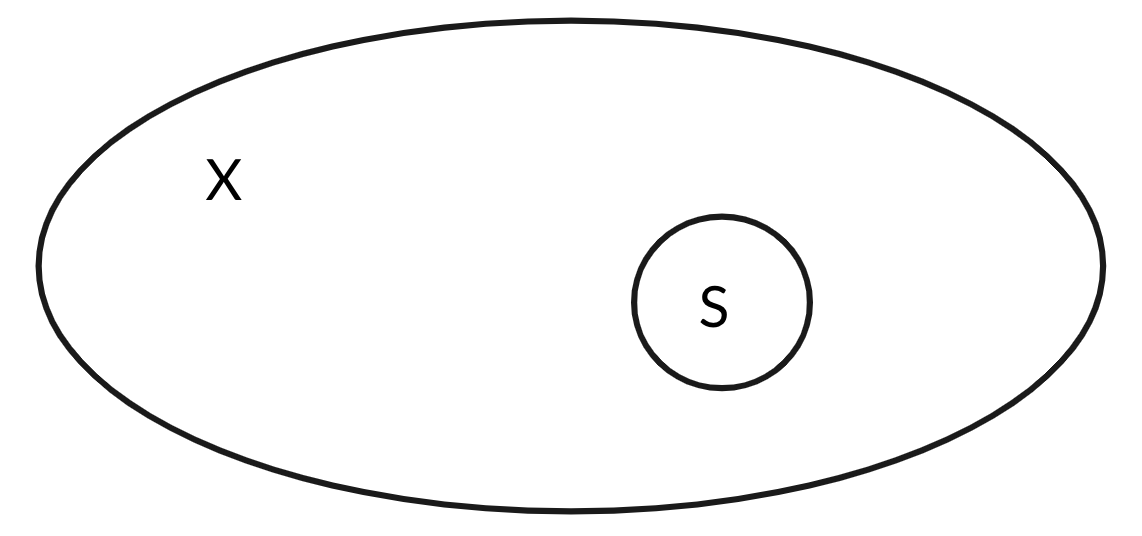
\includegraphics[origin=c,width=12cm]{../figures/independent-support.png}}
\caption{Visual Representation of an Independent Support}
\label{fig:ind_support}
\end{figure}

The primary target domain for UniGen is \textit{Constrained Random Verification} or CRV. In the domain of CRV, $|S|$ is typically significantly smaller than $|X|$, often by many orders of magnitude. UniGen exploits these observations by only applying variables in $S$ to the hash functions, which yields a significant reduction in the length of generated XOR clauses. Therefore UniGen indeed scales to formulas with hundreds of thousands of variables, and even millions of clauses, but \textit{only} when $|S|$ remains small, typically $|S| < 100$. In the UniGen benchmarks, UniGen generated samples for over 200 different formulas. The largest of these, \texttt{demo3\_new}, had $865,935$ variables and $3,509,158$ clauses, but $|S|$ was only $45$. Similarly, the largest value of $|S|$ in the benchmarks was $78$ in \texttt{diagStencil\_new}, with $94,607$ variables and $2,838,579$ clauses. \cite{chakraborty_parallel_2015}

How does $|S|$ grow in the formulas generated by SweetPea? SweetPea currently selects all variables that directly represent level values for each factor in each trial as the independent support. For example, in the encoding shown in Table \ref{tab:encoding_diagram}, all 72 variables would be included in the independent support. However, the independent support does not include variables used to encode additional constraints or intermediate variables introduced during Tseitin encoding. While this set does not grow factorially, it still quickly grows into the hundreds and thousands, as shown in table \ref{tab:benchmark_experiments_support}. While this independent support is certainly not minimal, we will see that even an optimal selection for the independent support could not guarantee $|S| < 100$.

\begin{table}[htb]
  \centering
  \caption{Independent Support Size for Benchmark Experiments}
\begin{tabular}{|c|c|}
\hline
\multicolumn{1}{|l|}{Experiment Name}  & $|S|$   \\ \hline
stroop-2                               & 24      \\ \hline
stroop-3                               & 72      \\ \hline
stroop-4                               & 160     \\ \hline
stroop-5                               & 300     \\ \hline
stroop-congruency-balanced             & 270     \\ \hline
stroop-response                        & 526     \\ \hline
padmala-pessoa                         & 1,303   \\ \hline
task-switching                         & 636     \\ \hline
task-switching-2                       & 2,770   \\ \hline
% task-switching-cue-switching           & 24,594  \\ \hline
\end{tabular}
\label{tab:benchmark_experiments_support}%
\end{table}



There are a few simple improvements that could be made to the independent support computation today. Rather than including the variables for \textit{all} factors and levels in the independent support, it could exclude variables for derived factors whose levels are constrained by other factors. Additionally, a more efficient SAT encoding could be used based on combinations of variables rather than representing all levels as individual variables. (Although this would increase the complexity of encoding constraints.) Both of these would reduce $|S|$ by a degree, allowing UniGen to be useful for slightly larger formulas.

For any formula $F$ with independent support $S$, there are, by definition, exactly $2^{|S|}$ distinct assignments to $F$. Therefore there can be no more than $2^{|S|}$ satisfying assignments, or solutions, to $F$. (In practice the number of solutions will be much less, as not \textit{all} possible assignments will satisfy the formula.) Assuming an upper-bound of $100$ for $|S|$, a perfectly efficient SAT encoding, and a minimal independent support, UniGen could only sample solutions to formulas with at most $2^{100}$ solutions. As seen in Table \ref{tab:benchmark_experiments}, SweetPea designs regularly exceed this threshold. Therefore UniGen alone is insufficient for generating solutions, regardless of any potential improvements to the SAT encoding or the independent support computation.

\subsection{Benchmarks}

This shortcoming is proved out in practice. UniGen fails to count or sample from formulas where $|S| > 100$. Table \ref{tab:benchmark_experiments_unigen} denotes the time required for UniGen to generate 10 samples for each experiment. An estimate for $|R_F|$ is provided manually based on the factorial of the sequence length. Nearly all of them fail to complete in the allotted time (10 hours).

% Time to sample with 10 samples
% python -m timeit "__import__('os').system('unigen --verbosity=0 --kappa=0.638 --pivotUniGen=27 --maxLoopTime=3000 --maxTotalTime=36000 --pivotAC=60 --gaussuntil=400 --samples=10 --startIteration=13 stroop-3.cnf stroop3-unigen.out')"
% python -m timeit "__import__('os').system('unigen --verbosity=0 --kappa=0.638 --pivotUniGen=27 --maxLoopTime=3000 --maxTotalTime=36000 --pivotAC=60 --gaussuntil=400 --samples=10 --startIteration=38 stroop-4.cnf stroop4-unigen.out')"

\begin{table}[htb]
  \centering
  \caption{Time to Generate 10 Samples with UniGen}
\begin{tabular}{|c|c|c|c|c|}
\hline
\multicolumn{1}{|l|}{Experiment Name} & Time to Sample  \\ \hline
stroop-2                              & -               \\ \hline
stroop-3                              & 2.18s           \\ \hline
stroop-4                              & Timed Out       \\ \hline
stroop-5                              & Timed Out       \\ \hline
stroop-congruency-balanced            & Timed Out       \\ \hline
stroop-response                       & Timed Out       \\ \hline
padmala-pessoa                        & Timed Out       \\ \hline
task-switching                        & Timed Out       \\ \hline
task-switching-2                      & Timed Out       \\ \hline
\end{tabular}
\label{tab:benchmark_experiments_unigen}
\end{table}


\section{Other Benchmarks}

As mentioned at the beginning of this chapter, we tested several other SAT samplers. This section presents the results of testing multiple SAT solving and sampling tools, as well as additional information on the implementation strategy of each tool. All sampling benchmarks were configured to generate ten samples at a time

\subsection{CryptoMiniSat}

CryptoMiniSat \cite{DBLP:conf/sat/SoosNC09,DBLP:conf/sat/2009} is a SAT solver. It is used internally by UniGen, as well as directly by SweePea to generate non-uniformly distributed trial sequences. SweetPea does non-uniform sampling by simply solving for any solution, then constraining the original formula to disallow that particular solution from being produced a second time. Due to the difficulty encountered while attempting to use SAT samplers, it has proven quite valuable to provide researchers with this ability to quickly generate some number of trial sequences conforming to their design, even though their distribution may be non-uniform. Sacrificing this guarantee allows them to quickly determine whether or not a particular design is even viable before investing additional resources. Lastly, in addition to logical \texttt{AND}, \texttt{OR}, and \texttt{NOT} clauses, CryptoMiniSat also natively supports \texttt{XOR} clauses, although SweetPea has not yet put these to use. (This is an opportunity for improvement.) Table \ref{tab:benchmark_experiments_cmsat} denotes the time required for CryptoMiniSat to compute a single solution to the SAT formula for each experiment.

% python -m timeit "__import__('os').system('cryptominisat5 padmala-pessoa.cnf > /dev/null')"

\begin{table}[htb]
  \centering
  \caption{Time to Solve for 1 Solution with CryptoMiniSat}
\begin{tabular}{|c|c|c|c|c|}
\hline
\multicolumn{1}{|l|}{Experiment Name} & Time to Solve (ms)  \\ \hline
stroop-2                              & 4.9                 \\ \hline
stroop-3                              & 9.1                 \\ \hline
stroop-4                              & 18.9                \\ \hline
stroop-5                              & 64.4                \\ \hline
stroop-congruency-balanced            & 23.9                \\ \hline
stroop-response                       & 232                 \\ \hline
padmala-pessoa                        & 3,380               \\ \hline
task-switching                        & 140                 \\ \hline
task-switching-2                      & 200,000             \\ \hline
\end{tabular}
\label{tab:benchmark_experiments_cmsat}
\end{table}

The most complicated design for which SweetPea was able to construct a CNF encoding (\texttt{task-switching-2}) took the longest, at 200 seconds. CryptoMiniSat solved all other experiments in less than a second. Since this tool only generates a single solution, the practical time consideration is of minor importance here.


\subsection{KUS}

KUS \cite{SGRM18} is another SAT sampler developed by some of the same team behind UniGen. However, it approaches the problem quite differently. Rather than using hash functions to partition the solution space, KUS requires a compiled deterministic decomposable negation normal form (d-DNNF) of a formula. There are known polynomial-time techniques for many operations on the d-DNNF representation of a boolean formula, including model counting. KUS takes advantage of these techniques to sample solutions using this form uniformly. This technique offloads much of the complexity to the d-DNNF compiler, rather than the sampling phase. KUS, while able to sample quickly, is not used in SweetPea due to scaling problems in compiling the d-DNNF form. Though the number of variables and clauses in the CNF for a formula is typically modest, compiling the equivalent d-DNNF has proven intractable. Table \ref{tab:benchmark_experiments_d4} denotes the time required to compile the CNF for each experiment to d-DNNF using the \texttt{d4} compiler, as well as the resulting d-DNNF file size,  compared to the original CNF file.

% TIme to compile d-DNNF
% Size of a d-DNNF file vs. original CNF, % increase in file size?

% Time to sample with 10 samples.
% time timelimit -T 36000 -t 36000 /home/drautb/GitHub/meelgroup/KUS/d4 cnfs/stroop-congruency-balanced.cnf -out=d-DNNFs/stroop-congruency-balanced.dnnf

% ➜  benchmark-experiments git:(master) ✗ time timelimit -T 36000 -t 36000 /home/drautb/GitHub/meelgroup/KUS/d4 cnfs/task-switching-2.cnf -out=d-DNNFs/task-switching-2.dnnf
% c WARNING: for repeatability, setting FPU to use double precision
% c Problem Statistics:
% c
% c Benchmark Information
% c Number of variables: 742832
% c Number of clauses: 2043674
% c Number of literals: 5958852
% c Parse time: 0.39
% c
% ===============================================================================
% INDETERMINATE
% timelimit -T 36000 -t 36000 /home/drautb/GitHub/meelgroup/KUS/d4    18709.93s user 7.88s system 99% cpu 5:12:08.05 total

\begin{table}[htb]
  \centering
  \caption{d-DNNF Compilation for Sampling with KUS}
\begin{tabular}{|c|c|c|c|c|}
\hline
\multicolumn{1}{|l|}{Experiment Name} & Time            & d-DNNF               & CNF            & \% Growth   \\ \hline
stroop-2                              & 14.4ms          & 9.7K                 & 24K            & -60\%       \\ \hline
stroop-3                              & 1.99s           & 6.3M                 & 151K           & 4,072\%     \\ \hline
stroop-4                              & Timed Out       & -                    & 303K           & -           \\ \hline
stroop-5                              & Timed Out       & -                    & 881K           & -           \\ \hline
stroop-congruency-balanced            & 48.6m           & 7.3G                 & 447K           & 1,633,009\% \\ \hline
stroop-response                       & Timed Out       & -                    & 1.5M           & -           \\ \hline
padmala-pessoa                        & OOM             & -                    & 13M            & -           \\ \hline
task-switching                        & Timed Out       & -                    & 1.2M           & -           \\ \hline
task-switching-2                      & "Indeterminate" & -                    & 92M            & -           \\ \hline % (5.2 hrs)
\end{tabular}
\label{tab:benchmark_experiments_d4}
\end{table}

For the experiments for which the d-DNNF compiler completed, table \ref{tab:benchmark_experiments_kus} denotes the time required to sample solutions using KUS.

% ➜  benchmark-experiments git:(master) ✗ time timelimit -T 36000 -t 36000 python /home/drautb/GitHub/meelgroup/KUS/KUS.py --dDNNF ~/Desktop/stroop-congruency-balanced.dnnf --samples 10 --outputfile d-DNNFs/stroop-congruency-balanced-kus-10-samples.out
% timelimit -T 36000 -t 36000 python /home/drautb/GitHub/meelgroup/KUS/KUS.py    11.39s user 11.16s system 5% cpu 7:05.45 total

\begin{table}[htb]
  \centering
  \caption{Time to Generate 10 Samples with KUS}
\begin{tabular}{|c|c|c|c|c|}
\hline
\multicolumn{1}{|l|}{Experiment Name} & Time        \\ \hline
stroop-2                              & 92.7 ms     \\ \hline
stroop-3                              & 2.35 s      \\ \hline
stroop-4                              & -           \\ \hline
stroop-5                              & -           \\ \hline
stroop-congruency-balanced            & OOM         \\ \hline  % 7mins 5s
stroop-response                       & -           \\ \hline
padmala-pessoa                        & -           \\ \hline
task-switching                        & -           \\ \hline
task-switching-2                      & -           \\ \hline
task-switching-cue-switching          & -           \\ \hline
\end{tabular}
\label{tab:benchmark_experiments_kus}%
\end{table}

As expected, sampling occurs quickly once a reasonably-sized d-DNNF file has been obtained. However, the combinatorial nature of experimental designs makes the cost of compiling and interpreting the d-DNNF prohibitive.


\subsection{Spur}

Spur \cite{spur} is a more recent SAT sampler that employs reservoir sampling. In benchmarks, it performs better than UniGen in nearly all cases. However, it does require an exact model count (based on sharpSAT), while an approximation suffices for UniGen. SweetPea does not rely on Spur at present, as it did not exist at SweetPea's inception. However, we consider it here as it represents the latest research for SAT sampling. Table \ref{tab:benchmark_experiments_spur} denotes the time required to generate samples for each experiment using Spur, with results similar to other tools.

% Time to get a model count.

% Time to sample 10 samples

% ➜  benchmark-experiments git:(master) ✗ time timelimit -T 36000 -t 36000 ~/GitHub/ZaydH/spur/build/Release/spur -cnf cnfs/task-switching-2.cnf -s 10
% WARNING: No sample results file specified.
% Using default filename: "cnfs/samples_task-switching-2.txt"
% Performing Uniform Model Sampling...
% Input File:  cnfs/task-switching-2.cnf
% Output File: cnfs/samples_task-switching-2.txt

% Preprocessing ... DONE
% variables (all/used/free):      742832/742832/0
% independent support size:       2770
% clauses (all/long/binary/unit): 3672632/3133493/384324/154815
% terminate called after throwing an instance of 'std::bad_alloc'
%   what():  std::bad_alloc
% timelimit -T 36000 -t 36000 ~/GitHub/ZaydH/spur/build/Release/spur -cnf  -s 1  71.16s user 6.95s system 62% cpu 2:04.49 total


\begin{table}[htb]
  \centering
  \caption{Time to Generate 10 Samples with Spur}
\begin{tabular}{|c|c|c|c|c|}
\hline
\multicolumn{1}{|l|}{Experiment Name} & Time to Sample                \\ \hline
stroop-2                              & 21.9 ms                       \\ \hline
stroop-3                              & 3.72 s                        \\ \hline
stroop-4                              & Timed Out                     \\ \hline
stroop-5                              & Timed Out                     \\ \hline
stroop-congruency-balanced            & OOM                           \\ \hline  % 5hrs 5mins
stroop-response                       & Error                         \\ \hline  % 7hrs 52mins
padmala-pessoa                        & Timed Out                     \\ \hline  % 10hrs
task-switching                        & Timed Out                     \\ \hline  % 10hrs
task-switching-2                      & Error                         \\ \hline  % 2hrs 5mins
task-switching-cue-switching          & -                             \\ \hline  % Don't have CNF
\end{tabular}
\label{tab:benchmark_experiments_spur}%
\end{table}

As with other Samplers, Spur can successfully generate samples for only the smallest designs.


\section{Sample Distribution}

As has been mentioned several times, there must be a one-to-one relationship between unique trial sequences and solutions to the SAT formula in order for uniformity guarantees to carry over from the SAT sampler results back to the original problem space. In this section, we will examine the distribution of the trial sequences produced by UniGen, KUS, and Spur, providing empirical evidence that the resulting trial sequences follow a uniform distribution.

We sampled 10,000 trial sequences for the Stroop-3 experiment using UniGen, KUS, and Spur. The resulting samples follow a uniform distribution; each sample only occurred once in the vast majority of cases.

\subsection{UniGen}

UniGen sampled 10,010 trial sequences, 9,965 of which were unique. Numbering each unique trial sequence in the order that it appeared and generating a histogram gives a visual confirmation that the sequences are approximately uniform. UniGen generated 333 sequences twice and only generated six three times. It generated no sequences more than three times.

\begin{figure}[htb]
\centering
\centerline{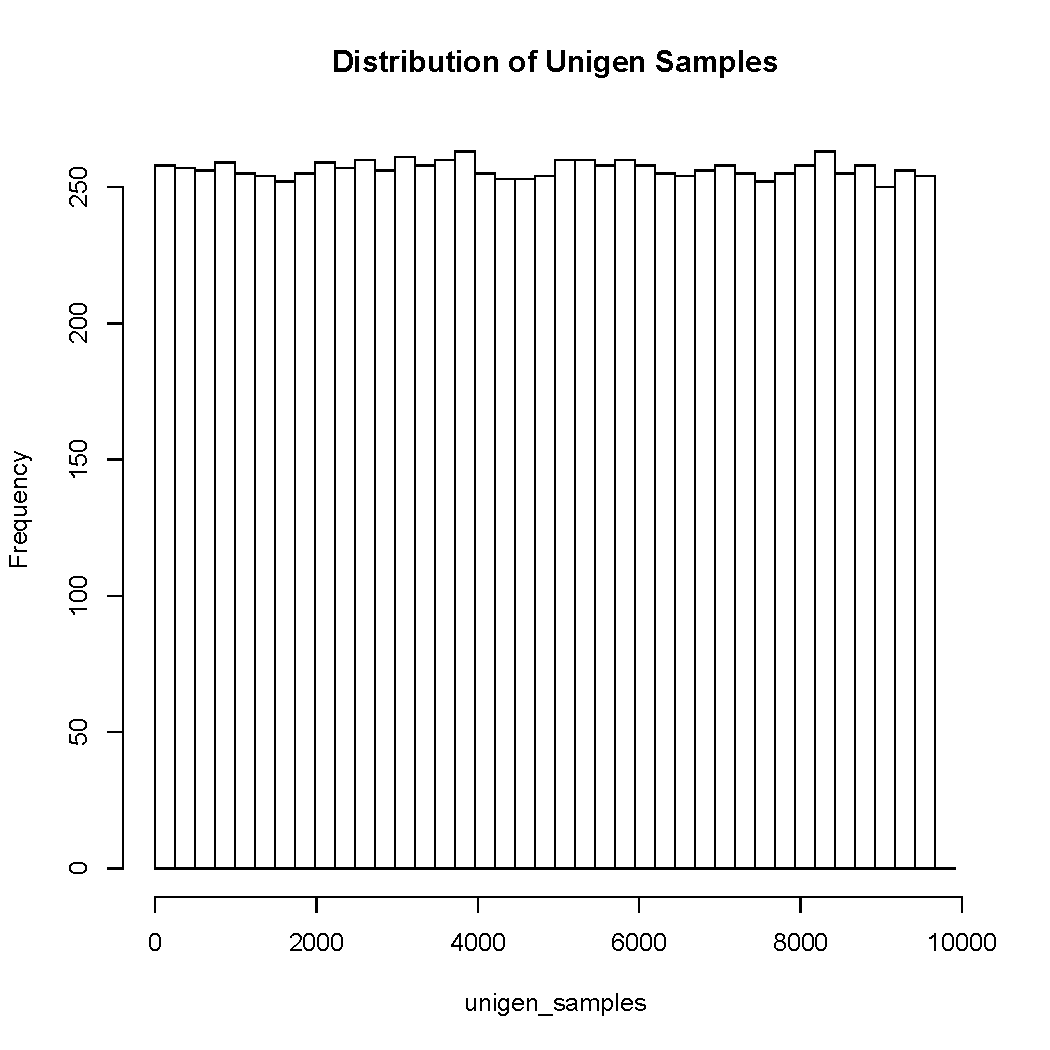
\includegraphics[origin=c,width=12cm]{../figures/unigen-samples.pdf}}
\caption{Distribution of Sequences Sampled by UniGen}
\label{fig:unigen_samples}
\end{figure}


\subsection{KUS}

% time python /home/drautb/GitHub/meelgroup/KUS/KUS.py --dDNNF d-DNNFs/stroop-3.dnnf --samples 10000 --outputfile d-DNNFs/stroop-3-kus-10000-samples.out
% ('Time taken to parse the nnf text:', 1.0481359958648682)
% ('Time taken for Model Counting:', 1.0421910285949707)
% ('Model Count:', 112409849997702614628L)
% ('Time taken by sampling:', 16.441092014312744)
% ('Samples saved to', 'd-DNNFs/stroop-3-kus-10000-samples.out')
% python /home/drautb/GitHub/meelgroup/KUS/KUS.py --dDNNF d-DNNFs/stroop-3.dnnf  25.76s user 0.59s system 102% cpu 25.828 total

KUS sampled 10,000 trials sequences, all of which were unique.

\begin{figure}[htb]
\centering
\centerline{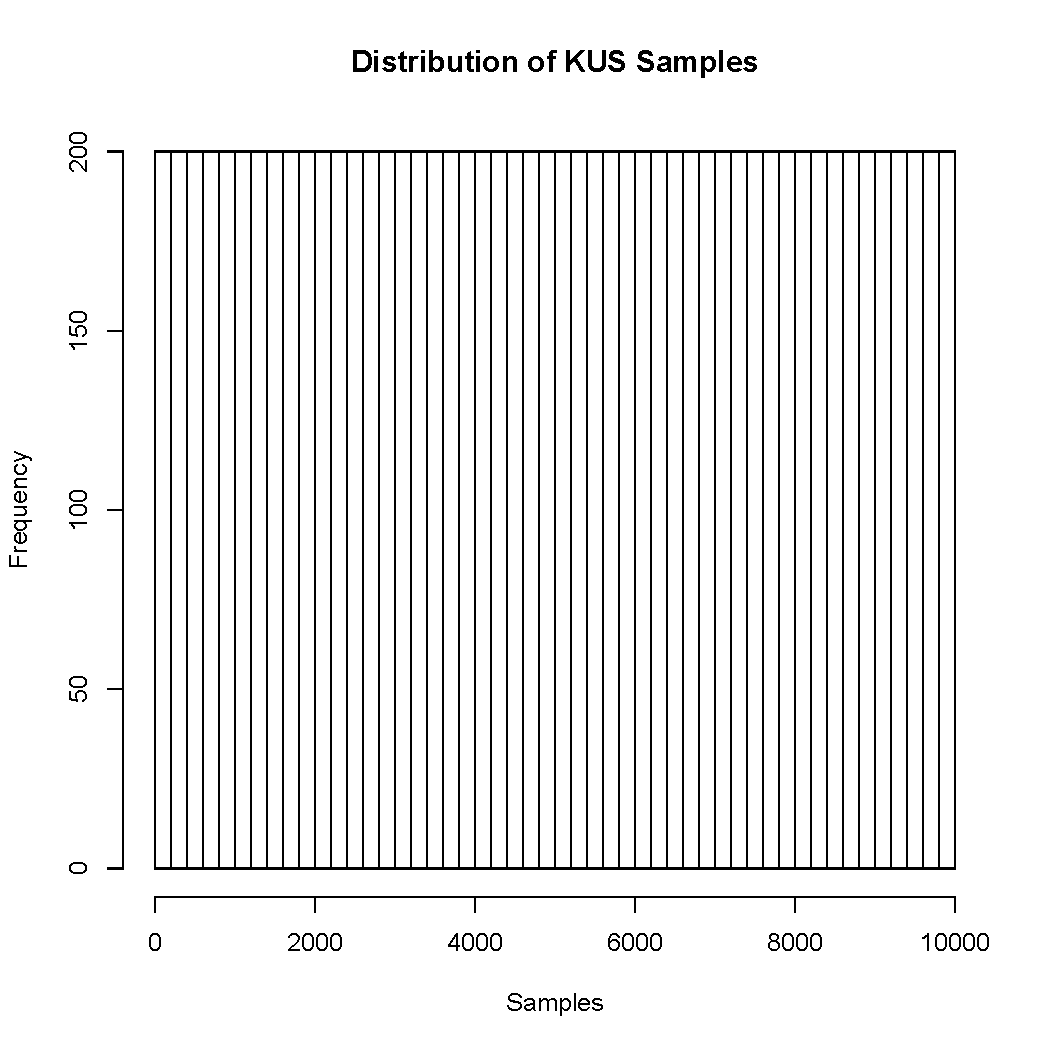
\includegraphics[origin=c,width=12cm]{../figures/kus-samples.pdf}}
\caption{Distribution of Sequences Sampled by KUS}
\label{fig:kus_samples}
\end{figure}


\subsection{Spur}

% time /home/drautb/GitHub/ZaydH/spur/build/Release/spur -q -s 10000 -cnf stroop-3.cnf -out stroop-3-spur-10000-samples.out
% /home/drautb/GitHub/ZaydH/spur/build/Release/spur -q -s 10000 -cnf  -out   30.97s user 0.23s system 99% cpu 31.250 total

Spur sampled 10,000 trial sequences, 9,664 of which were unique. It generated three hundred thirty-two sequences twice and two sequences three times. It generated no sequences more than three times.

\begin{figure}[htb]
\centering
\centerline{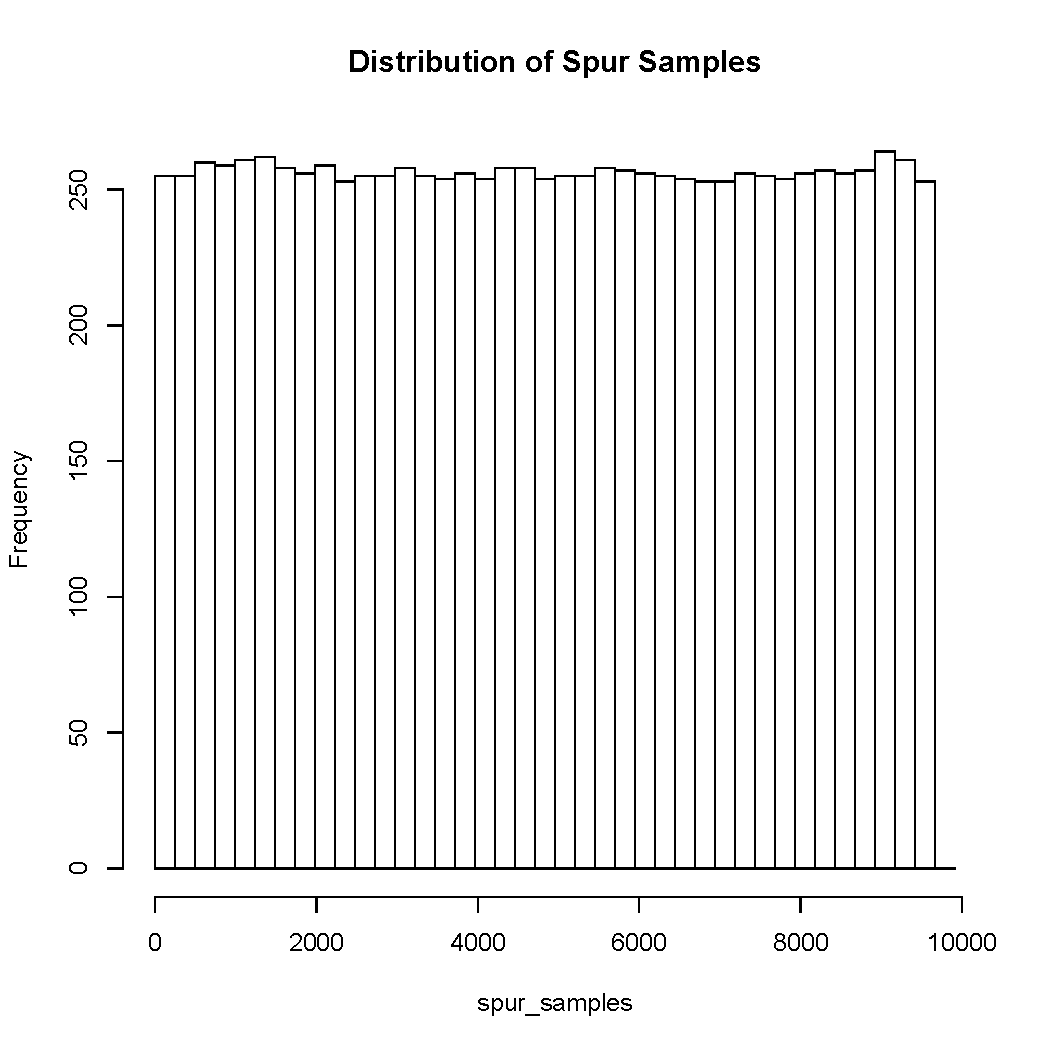
\includegraphics[origin=c,width=12cm]{../figures/spur-samples.pdf}}
\caption{Distribution of Sequences Sampled by Spur}
\label{fig:spur_samples}
\end{figure}

\subsection{CryptoMiniSat}

In contrast to the previous tests, when a SAT solver is used to generate individual samples incrementally by adding negated solutions to the prior formula, the same samples are generated each time. We used CryptoMiniSat to generate 10,000 samples as well, in groups of 100. It generated precisely the same set of 100 samples each time.


Of all the Samplers tested, KUS produced the most uniformly distributed samples.

\section{Summary}

We had hoped that UniGen would be able to generate uniformly-distributed solutions for experimental designs, in particular because the volume of variables and clauses in our generated CNF files fell within the range of example benchmarks provided by the UniGen authors. However, we overlooked the role played by the magnitude of the independent support set. Because UniGen requires the size of the independent support set to be less than 100 variables, there is a limit to the number of solutions a formula may have in order for UniGen to be effective. For realistic experimental designs, the number of solutions quickly outstrips this bound. Furthermore, none of the additional tested tools for sampling SAT formulae are capable of handling the scale of practical experimental designs. Although these experiments contain a reasonable number of variables and clauses, the factorial explosion in the solution space, as well as the magnitude of the independent support set, proved too large.

%%% -*-LaTeX-*-

\chapter{Solution Counting}

Today, SweetPea offloads the entire sampling process to an external tool. While an attractive option from an implementation standpoint, this strategy does not scale to the degree needed by SweetPea. As demonstrated in Chapters 1 and 3, the solution spaces from which SweetPea is trying to sample are beyond the capacity of any existing tools. One of the shortcomings of this approach is that external tools cannot exploit domain knowledge of the problem to guide their decisions.

One may view experimental designs in SweetPea as combinatorics problems, each with a countable set of solutions. If a formula for counting the solutions to an experimental design could be derived, then it may also be possible to discover a bijection between solutions to the design and the natural numbers. If a corresponding natural number could uniquely identify every possible solution, then we could guarantee uniformity by randomly sampling natural numbers from the uniform distribution. As a first foray into solution counting, this chapter presents such a formula for tier one, two, and three designs. This exploration will also defer treatment of the set of external design constraints.


\section{Principles of Counting}

Before describing a formula for counting solutions to experimental designs, it will be useful to review a few counting principles for future reference, beginning with counting permutations of a set. As explained by Brualdi \cite{brualdi_introductory_2010}, the standard formula for computing the number of permutations of $r$ items taken from an $n$-element set is:

\[
P(n,r) = \frac{n!}{(n-r)!}
\]

When $n =  r$, this becomes simply $n!$.

% Similary, the number of combinations of $r$ items from an $n$-element set is:

% \[
% {n \choose r} = \frac{n!}{r!(n-r)!}
% \]

When constructing a set $S$ by combining individual elements from mulitple other sets, $P_1, P_2, \cdot\cdot\cdot P_n$, the size of $S$ is the product of the sizes of sets $P_1, P_2, \cdot\cdot\cdot P_n$:

\[
|S| = \prod_{i=1}^n |P_i|
\]

This is known as the \textit{Multiplication Principle} \cite{brualdi_introductory_2010}. Both of these principles will be used to calculate the number of solutions to a SweetPea design.


\section{Partition of an Experimental Design}

An experimental design is composed of three elements: a set of factors, a subset of the factors that form the crossing, and a set of constraints. The set of crossed factors fundamentally shapes the generated trial sequences. The number of combinations of level values taken from each crossed factor governs the length of a trial sequence. For example, consider a design in which there are two crossed factors, each with three levels. By the multiplication principle, there are $3 * 3 = 9$ unique combinations of level values from each factor in the crossing; hence, trial sequences in this design will be nine trials long. The sequence length is a critical factor in the solution count, as are other factors that are not in the crossing.

To formalize the relationship between each factor and the total solution count, we define a partition for the set of factors in the design. Let $D$ be the set of all factors in the design. Let $C$ be the set of factors that form the crossing, and $\overline{C}$ be the set of factors not included in the crossing. Therefore, $C \subseteq D$ and $\overline{C} \subset D$. We can further divide $C$ and $\overline{C}$ by basic and derived factors. Let $C_B$ be the set of basic factors in $C$, and $C_D$ be the set of derived factors in $C$. $\overline{C}_B$ and $\overline{C}_D$ are defined as the basic factors not in the crossing and the complex factors not in the crossing, respectively.

Lastly, we further divide $\overline{C}_B$ into two more sets. Although the set of crossed factors does not include basic factors in $\overline{C}$, this does not imply that they are fully independent. Factors in $\overline{C}_B$ may contribute to the selected levels for factors in $C_D$. We will refer to these factors in $\overline{C}_B$ as \textit{source} factors, as they are at least a partial source of data controlling factors in $C_D$. We will group such factors in $\overline{C}_{B_S}$, while $\overline{C}_{B_I}$ represents the truly independent basic factors in $\overline{C}$.

We could also define $C_{B_S}$ and $C_{B_I}$; however, there is no benefit to doing so. Because the crossing is the highest source of authority, the relationship between factors in $C_B$ and dependent derived factors is inverted. Each combination of levels in the crossed set governs the values for $C_B$, which will then, in turn, govern dependent derived factors.

The partition of $D$ with which we are concerned is therefore: $\{C_B, C_D, \overline{C}_{B_S}, \overline{C}_{B_I}, \overline{C}_D\}$. A visual hierarchy of this partition is shown in Figure \ref{fig:partition}.

% \begin{figure}[t]
% \centering
% \centerline{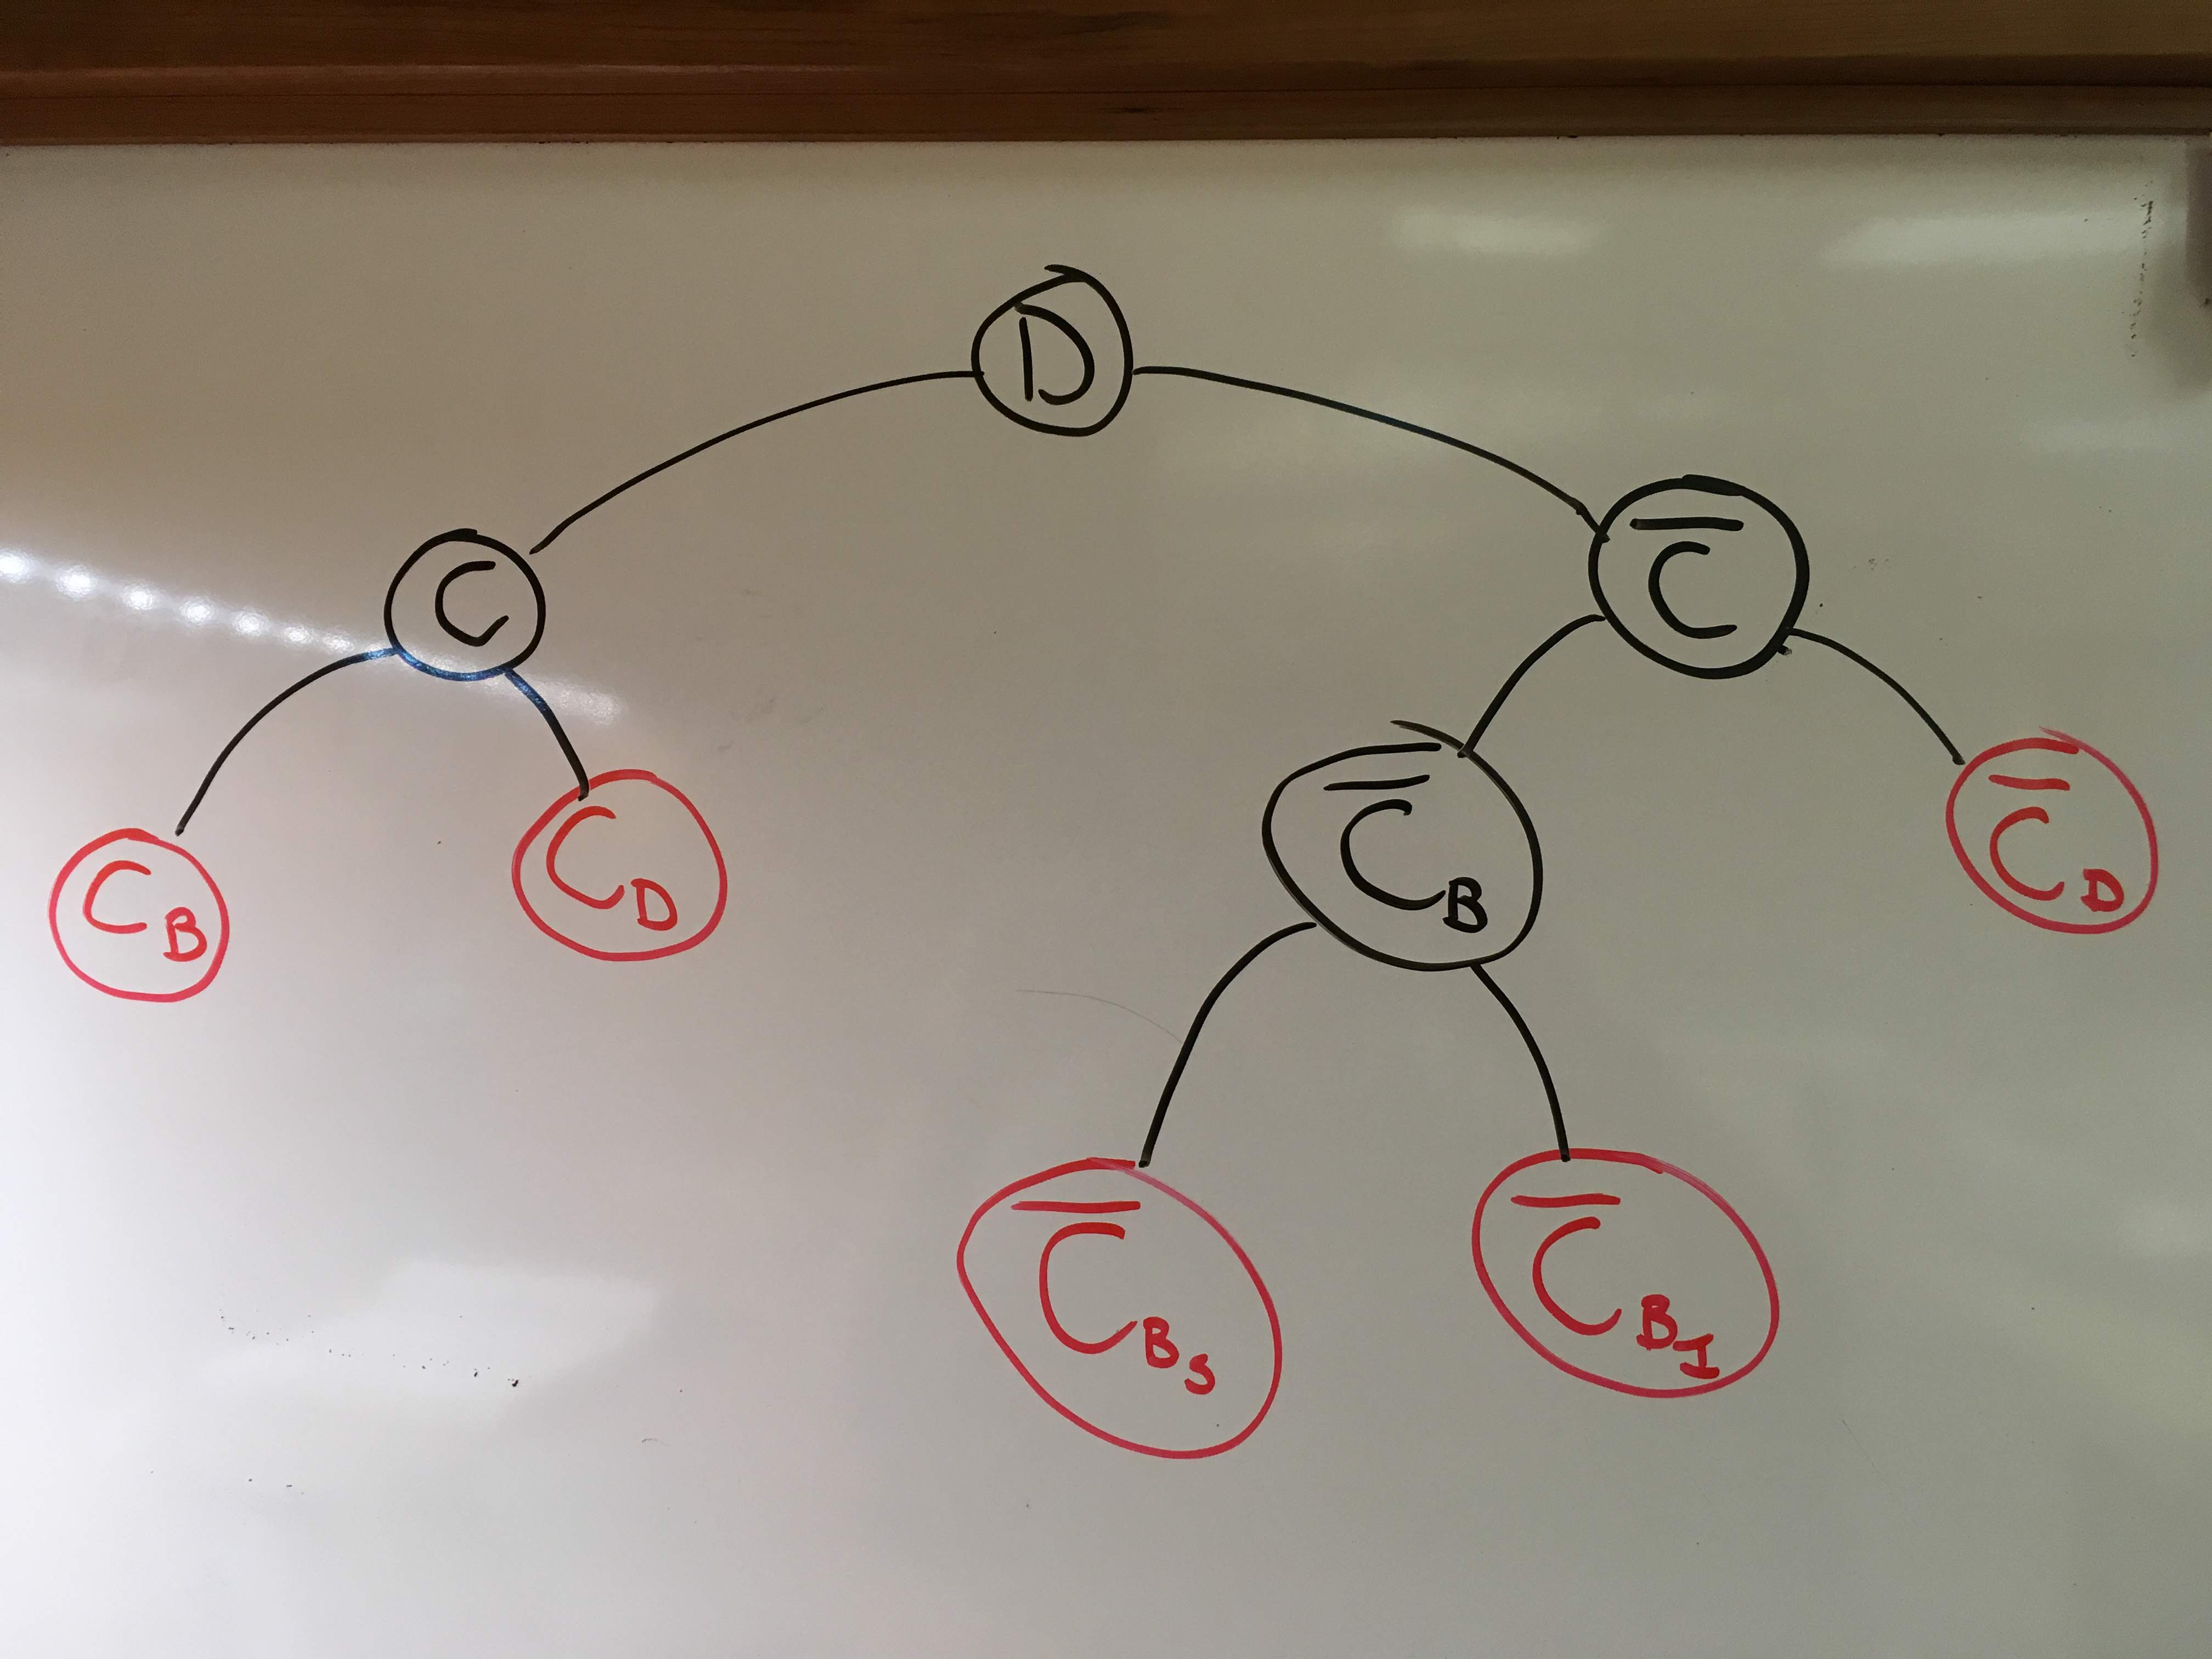
\includegraphics[origin=c,width=12cm]{../figures/partition.jpg}}
% \caption{Partition of an Experimental Design}
% \label{fig:partition}
% \end{figure}

\begin{figure}[b]
\centering
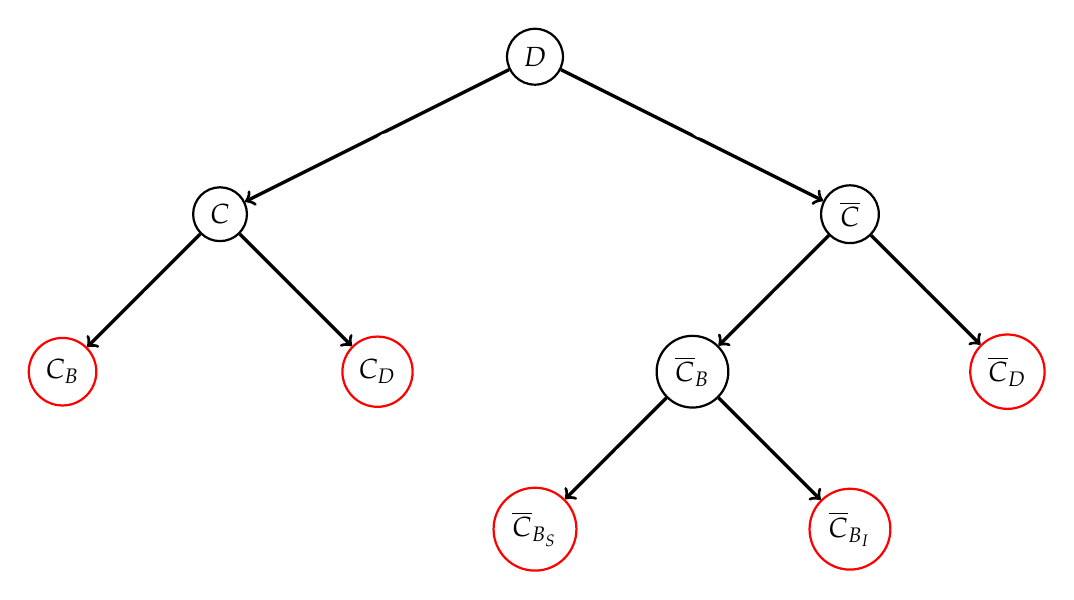
\begin{tikzpicture}[auto]
\begin{scope}[every node/.style={circle,thick,draw}]
    \node (D) at (8,8) {$D$};

    \node (C) at (4,6) {$C$};
    \node (CBar) at (12,6) {$\overline{C}$};

    \node[draw=red] (CB) at (2,4) {$C_B$};
    \node[draw=red] (CD) at (6,4) {$C_D$};
    \node (CBarB) at (10,4) {$\overline{C}_B$};
    \node[draw=red] (CBarD) at (14,4) {$\overline{C}_D$};

    \node[draw=red] (CBarBS) at (8,2) {$\overline{C}_{B_S}$};
    \node[draw=red] (CBarBI) at (12,2) {$\overline{C}_{B_I}$};
\end{scope}

\begin{scope}[every node/.style={fill=white,circle},
              every edge/.style={draw=black,very thick}]
    \path [->] (D) edge node {} (C);
    \path [->] (D) edge node {} (CBar);

    \path [->] (C) edge node {} (CB);
    \path [->] (C) edge node {} (CD);

    \path [->] (CBar) edge node {} (CBarB);
    \path [->] (CBar) edge node {} (CBarD);

    \path [->] (CBarB) edge node {} (CBarBS);
    \path [->] (CBarB) edge node {} (CBarBI);
\end{scope}
\end{tikzpicture}
\caption{Partition of an Experimental Design}
\label{fig:partition}
\end{figure}


Lastly, we establish notation for referrings to individual level combinations in $C$. Let $X$ be a set of sequences $t_1, t_2, \cdot\cdot\cdot t_n$, representing the combinations of levels for all factors in $C$. Each sequence $t$ contains items $i_1, i_2, \cdot\cdot\cdot i_j$, where item $i_j$ is one of the levels from the $j_{th}$ factor in $C$. Each sequence $t$ must be unique, and there is an sequence for every possible combination of levels from factors in $C$.

Recall the earlier design example with factors to represent the color and text of a printed word. Both the color and text factors had three levels: \texttt{red}, \texttt{green}, and \texttt{blue}. For this crossing, $X$ can be visualized in Table \ref{tab:sequences}.

\begin{table}[htb]
  \centering
  \caption{Expressing Level Combinations as Sequences}
\begin{tabular}{|c|cc|}
\hline
\textbf{}      & \textbf{$i_1$} & \textbf{$i_2$} \\ \hline
\textbf{$t_1$} & red            & red            \\
\textbf{$t_2$} & red            & green          \\
\textbf{$t_3$} & red            & blue           \\
\textbf{$t_4$} & green          & red            \\
\textbf{$t_5$} & green          & green          \\
\textbf{$t_6$} & green          & blue           \\
\textbf{$t_7$} & blue           & red            \\
\textbf{$t_8$} & blue           & green          \\
\textbf{$t_9$} & blue           & blue           \\   \hline
\end{tabular}
\label{tab:sequences}
\end{table}

By the multiplication principle, there will be $n = C_1 \cdot C_2 \cdot\cdot\cdot C_{|C|}$ such sequences, and there are $P(n, n) = n!$ permutations of this set. We will also use $l$ to refer to the trial sequence length, which is equivalent to $|X|$.


\section{Formula}

With the partition established, we can develop the formula for counting the number of solutions, $s$, for a given experimental design. We will first derive the formula for a tier 1 design, and then add additional terms for tier 2 and tier 3 designs.

\subsection{Tier 1}

For tier 1 designs, the sequences in $X$ fully represent all possible level combinations in the design. $C_B \neq \emptyset$, while every other set in the partition is empty. The only variation between trial sequences is the ordering of pairs in $X$. Therefore, every permutation of $X$ represents a unique trial sequence, which means there are $s = l!$ solutions to a tier 1 design.

\subsection{Tier 2}

Tier 2 designs allow basic factors that are not in $C$, and are thus less constrained. In other words, starting with tier 2, $\overline{C}_{B_I} \neq \emptyset$. For a factor $f$, let $|f|$ denote the number of levels that $f$ has. For each $f \in \overline{C}_{B_I}$, $f$ is fully independent; therefore, any of the $|f|$ levels may be selected for each trial. In a sequence of $l$ trials, applying the multiplication principle reveals that there are $|f|^l$ possible sequences of levels of $f$. If $|\overline{C}_{B_I}| > 1$, then the multiplication principle is applied repeatedly to determine the total number of combinations for all factors in $\overline{C}_{B_I}$. Applying the multiplication principle a final time produces the final formula for tier 2:

\[
s = l! \cdot \prod_{i=1}^{|\overline{C}_{B_I}|} |f_i|^l
\]

\subsection{Tier 3}

Tier 3 designs allow the addition of derived factors. It is now possible that all sets in the partition are non-empty. $C_D$, $\overline{C}_{B_S}$, and $\overline{C}_D$ are the only sets in the partition remaining to account for. The presence of factors in $C_D$ does not alter the formula, as level selection for factors in $C_D$ is still controlled by $X$ (the crossing), regardless of their relationship to other factors. $\overline{C}_D$ also requires no special treatment as the level selection for uncrossed derived factors depends entirely on the levels selected for basic factors (regardless of whether the basic factors are in $C_B$, $\overline{C}_{B_S}$, or $\overline{C}_{B_I}$). Only $\overline{C}_{B_S}$ remains, containing the uncrossed basic factors that feed crossed derived factors.

Derived factors allow the user to provide an arbitrary predicate for each level in the factor. SweetPea applies these predicates to every combination of levels that could be given as arguments, effectively constructing a truth table, to determine which level to select for each combination of arguments. We define $X_S$ to be the set of sequences representing the crossing of factors in $\overline{C}_{B_S}$, also referred to as the \textit{source crossing}. The next task is to determine, for every element in $X$, which elements of $X_S$ are compatible using the user-defined predicates. Checking compatibility is necessary as some combinations in $X$ may preclude certain combinations in $X_S$.

For every sequence $t \in X$, there is some number of elements in $t$ corresponding to derived factor levels, labeled $d_1, d_2, \cdot\cdot\cdot d_{|C_D|}$ comprising the set $V_t$. Each $d \in V$ is associated with a predicate,\footnote{These predicates, also called derivation functions, are expected to be deterministic. If they are non-deterministic, then inconsistent solutions may be produced as the predicates may be applied more than once to the same arguments. SweetPea could minimize this concern by ensuring that each predicate is only applied once to each argument combination and then caching the results.} $pred(d)$. For every $t \in X$, every $b \in X_S$ is consulted to see if the predicates for all $d \in V_t$ are satisfied.\footnote{If $X$ is very large, then testing all combinations could become intractable. However, in practice, $X$ is relatively small, typically $|X| < 500$. Additionally, SweetPea's current implementation relies on $X$ being small enough for this to work, as it follows a similar process when generating the SAT encoding for derived factors.} If any of them is not satisfied, then $b$ is not a compatible choice for $t$ and must be discarded from consideration for $t$. Once this process is complete, a list of subsets of $X_S$ remains, in which the $n^{th}$ subset indicates which elements of $X_S$ are compatible with the $n^{th}$ crossing in $X$.

More formally, let $S$ be a list of items $J_1, J_2, \cdot\cdot\cdot J_{|X|}$. The following statements are true:

\begin{enumerate}
\item $\forall J \in S \mid J \subseteq X_S$
\item $\forall t \in X,  \forall d \in V_t \mid pred(d) \implies \top$
\end{enumerate}

Once we have generated $S$, we can apply the multiplication principle once more to complete the formula for tier 1, 2, and 3 designs:

\[
s = l! \cdot \prod_{i=1}^{|\overline{C}_{B_I}|} |f_i|^l \cdot \prod_{k=1}^{|S|} |J_k|
\]

The total number of solutions $s$ for a given experimental design is the product of the number of permutations of the crossing, the number of combinations of each independent factor, and the number of acceptable combinations of all source factors.

It is possible for the user to specify a crossing that is not satisfiable. Referring back to the Stroop example, the user may include all three factors, \texttt{color}, \texttt{text}, and \texttt{congruent}, in the crossing. This is unsatisfiable because some level combinations violate the rules of the derived factor. For example, \texttt{color=red}, \texttt{text=blue}, and \texttt{congruent=yes} is invalid because \texttt{red} and \texttt{blue} are not congruent according to the predicates for \texttt{congruent}. If such a crossing is specified, the formula for $s$ will correctly identify the number of potential solutions as zero.

\section{Example}

Consider a design composed of the same factors as the Stroop example:

\begin{verbatim}
color = Factor("color", ["red", "green", "blue"])
text  = Factor("text",  ["red", "green", "blue"])

congruent = Factor("congruent?", [
    DerivedLevel("yes", WithinTrial(operator.eq, [color, text])),
    DerivedLevel("no",  WithinTrial(operator.ne, [color, text]))
])
\end{verbatim}

However, rather than crossing \texttt{color} and \texttt{text}, we will demonstrate an example in which \texttt{color} and \texttt{congruent?} are crossed. For this design, the partition of $D$ becomes:

\begin{gather*}
    C_B = \{\texttt{color}\} \quad C_D = \{\texttt{congruent?}\}  \quad  \overline{C}_{B_S} = \{\texttt{text}\} \\
    \overline{C}_{B_I} = \emptyset \qquad\qquad \overline{C}_D = \emptyset
\end{gather*}

The crossing, or $X$, is the cartesian product of levels of \texttt{color} and \texttt{congruent?}. SweetPea generates this product exhaustively.

\begin{align*}
X = \{(red, yes), (red, no), (green, yes), (green, no), (blue, yes), (blue, no)\}
\end{align*}

The size of the crossing determines the sequence length; therefore, $l = |X| = 6$. As a result, the first term, $l!$, becomes $6! = 720$.

In this design, there are no basic independent factors outside the crossing: $\overline{C}_{B_I} = \emptyset$. Therefore, there is no value for the second term.

For the third and final term, we need to first determine $X_S$, the cartesian product of levels of factors in $\overline{C}_{B_S}$. For this design, the only factor in $\overline{C}_{B_S}$ is \texttt{text}. As a result, $X_S$ is simply the levels in \texttt{text}:

\[
X_S = \{red, green, blue\}
\]

At this point, each element of the product of $X$ and $X_S$ must be checked for validity under the derived factor definitions in the design to determine the subsets of $X_S$ that are valid for each element in $X$. In terms of this example, which level selections in $X_S$ do \textit{not} violate the definition of \texttt{congruent?} when paired with each level selection combination in $X$? These subsets comprise $S$ as defined in Section 4.3.3. Table \ref{tab:example_s} gives a visual representation of this process.

\begin{table}[b]
  \centering
  \caption{Computing $S$ for Solution Counting}
\begin{tabular}{r|c|c|c|c}
\cline{2-4}
\multicolumn{1}{c|}{}              & \multicolumn{3}{c|}{$X_S$}                 & \multicolumn{1}{l}{}                     \\ \hline
\multicolumn{1}{|c|}{$X$}          & red          & green        & blue         & \multicolumn{1}{c|}{$J$}                 \\ \hline
\multicolumn{1}{|r|}{(red, yes)}   & $\checkmark$ &              &              & \multicolumn{1}{c|}{$\{(red\}$}         \\ \hline
\multicolumn{1}{|r|}{(red, no)}    &              & $\checkmark$ & $\checkmark$ & \multicolumn{1}{c|}{$\{(green, blue)\}$} \\ \hline
\multicolumn{1}{|r|}{(green, yes)} &              & $\checkmark$ &              & \multicolumn{1}{c|}{$\{(green\}$}       \\ \hline
\multicolumn{1}{|r|}{(green, no)}  & $\checkmark$ &              & $\checkmark$ & \multicolumn{1}{c|}{$\{(red, blue)\}$}   \\ \hline
\multicolumn{1}{|r|}{(blue, yes)}  &              &              & $\checkmark$ & \multicolumn{1}{c|}{$\{(blue\}$}        \\ \hline
\multicolumn{1}{|r|}{(blue, no)}   & $\checkmark$ & $\checkmark$ &              & \multicolumn{1}{c|}{$\{(red, green)\}$}  \\ \hline
\end{tabular}
\label{tab:example_s}%
\end{table}

$S$ is therefore:

\[
S = \{(red), (green, blue), (green), (red, blue), (blue), (red, green)\}
\]

With $S$ defined, we may now compute the third term of the formula:
\[
    \prod_{k=1}^{|S|} |J_k| = 1 \cdot 2 \cdot 1 \cdot 2 \cdot 1 \cdot 2 = 8
\]

This yields the final solution count of $s = 720 \cdot 8 = 5,760$. One may confirm this solution by generating the corresponding SAT encoding for this design and applying a model counter to the generated CNF.

\section{Conclusion}

In this chapter, we derived a formula for counting the number of solutions to SweetPea designs in tiers 1, 2, or 3. However, this formula does not account for the third component of a design: constraints. Including constraints in the formula is beyond the scope of this thesis, as it would involve complexity similar to counting solutions for tier 4 and five designs. The formula, therefore, produces an exact solution count for designs lacking constraints and produces an upper-bound for designs with constraints. Next, we will apply the counting formula to construct uniformly-distributed trial sequences without relying on a SAT sampler.

% TODO: Correctness proof? Mention that we tested counts with SAT model counters?

%%% -*-LaTeX-*-

\chapter{Sequence Construction}

With an exact count of viable sequences for tier one, two, and three designs, a mapping from natural numbers to valid trial sequences is now a possibility. Such a mapping would prove valuable for guaranteeing a uniform distribution of samples, as well as generating solutions more efficiently. This chapter presents an algorithm that is guaranteed to generate uniformly-distributed solutions to tier one, two, and three designs. This is accomplished by randomly sampling natural numbers from the uniform distribution in the range of $[0, s)$, then generating the unique trial sequence associated with that number. Lastly, the generated trial sequence is checked against design constraints (if any exist), to ensure that no violations exist in the generated sequence.


\section{Enumerating Permutations and Combinations}

There are several steps involved in constructing a solution based on a natural number. In this section, we will review methods for generating the $n^{th}$ permutation or combination of a set, as well as mapping individual natural numbers to a unique set of numbers that covers the same space using modular arithmetic. These techniques form the basic building blocks for the final construction algorithm.

\subsection{Interval Mapping}

The construction algorithm will repeatedly need to take a single number and map it into a unique combination of multiple numbers, each from a possibly different range. We will refer to this process as \textit{interval mapping}.

Suppose we have $n$ numeric intervals, each ranging from $[0, r_n)$. Revisiting the multiplication principle, we can see that there are $m = \prod_1^n r_n$ unique combinations of individual values from each interval. If $j$ is a number selected from $[0, m)$, we can map $j$ to its unique combination of interval value selections using the modular arithmetic. (This technique will still work even when $j \geq m$, but combinations will begin to repeat.)

We begin by computing $j \bmod r_1$, and saving the result as the selection for the first interval. We then recompute $j$ to be $j = \lfloor \frac{j}{r_1} \rfloor$ before moving on to the next range. This process is repeated for $r_2,r_3,...,r_n$ until the full combination is developed. For example, if we had $U = \{3, 2, 4\}$ as the set of upper bounds for each interval, then there would be $3 \cdot 4 \cdot 2 = 24$ possible combinations of interval values. Suppose we want to compute the interval selections for $15$. This would be done as follows:

\begin{align*}
j = 15   &&  R_1 = 15 \bmod 3 = 0  &&  j = \Bigl\lfloor \frac{15}{3} \Bigr\rfloor = 5   \\
j = 5    &&  R_2 = 5 \bmod 4 = 1   &&  j = \Bigl\lfloor \frac{5}{4} \Bigr\rfloor = 1    \\
j = 1    &&  R_3 = 1 \bmod 2 = 1   &&                                                   \\
\end{align*}

Thus the set of selected values from each interval is $R = \{0, 1, 1\}$. Figure \ref{fig:interval_breakdown} demonstrates this visually.

\begin{figure}[htb]
\centering
\centerline{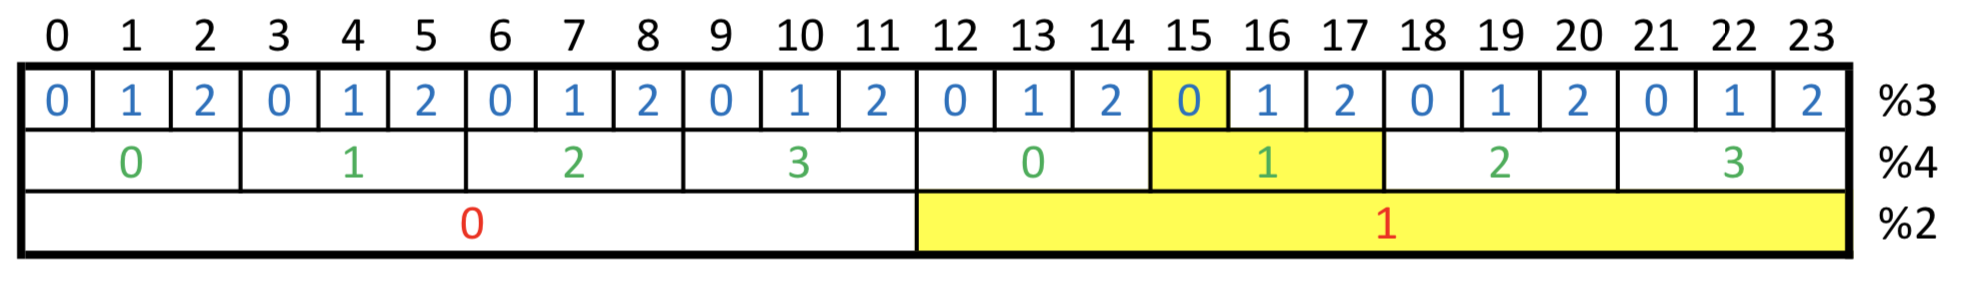
\includegraphics[origin=c,width=12cm]{../figures/interval-breakdown-final.png}}
\caption{Decomposing a Number into Constituent Ranges}
\label{fig:interval_breakdown}
\end{figure}

This technique will be applied multiple times during sequence construction to select a unique combination of values corresponding to a single integer.

\subsection{Constructing Permutations}

The construction algorithm also needs to map an individual number to a corresponding permutation of a set. Every permutation of a set can be identified by its \textit{inversion} or \textit{inversion sequence}. Loosely defined, the inversion sequence indicates how out-of-order the permutation is when compared with the original sequence. The concept of an inversion was first introduced by Hall \cite{hall_automorphisms_1962}, though we will use on Brualdi's description \cite{brualdi_introductory_2010} here.

Let $S$ be the set of numbers $\{1, 2, ..., n\}$ Suppose we have some permutation $p$ of $S$, $i_1, i_2, ..., i_n$. For each $i$, there exists some finite number of elements in $S$ whose values are greater than $i$, yet precede $i$ in $p$. This is called the inversion for $i$. An inversion sequence, $a_1, a_2, ... a_n$, is the sequence of inversions for a particular permutation of $S$.

For example, because the elements $\{1, 2, 3, 4, 5\}$ are in order, the corresponding inversion sequence for this arrangement is $\{0, 0, 0, 0, 0\}$. If we permute the sequence to obtain $\{2, 5, 4, 1, 3\}$, the associated inversion sequence is $\{3, 0, 2, 1, 0\}$. This sequence can be interpreted to mean that three elements larger than one precede one, zero elements larger than two precede two, two elements larger than three precede three, one element larger than four precedes four, and zero elements larger than five precede five. In our case, the original sequence will always be ascending; therefore, the last inversion must always be zero.

An inversion sequence can be used to generate the associated permutation by using the inversions to select where to place each element. Given an inversion sequence $a_1, a_2, ... a_n$, begin with $n$ empty locations. Beginning with $a_1$, skip $a_i$ empty locations before inserting the $i^{th}$ element of $S$. Figure \ref{fig:inversion_sequence} demonstrates this algorithm in the previous example.

\begin{figure}[htb]
\centering
\centerline{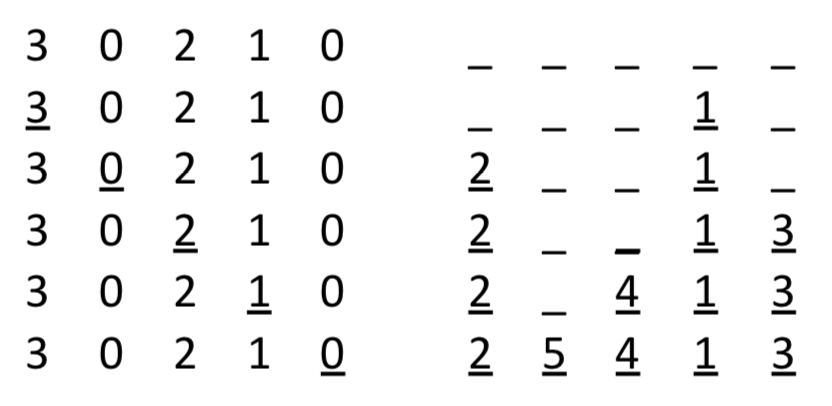
\includegraphics[origin=c,width=12cm]{../figures/inversion-sequence.png}}
\caption{Construction of a Permutation from its Inversion Sequence}
\label{fig:inversion_sequence}
\end{figure}

Finally, we can construct the inversion sequence for the $j^{th}$ permutation of a set by applying the interval mapping technique introduced previously. The maximum value of each position in the inversion sequence is used to construct the intervals. To construct an inversion sequence of $n$ inversions, the set of upper bounds for the intervals is $U = \{n, n - 1, n - 2, ..., 2, 1\}$. Using interval mapping to construct an inversion sequence, we can deterministically construct any permutation of a set.

\subsection{Combinations}

We can enumerate combinations of a set of elements in a similar manner. For a combination of $r$ elements, taken from a set of $k$ elements, the multiplication principle dictates that there are $k^r$ possibilities. Applying interval mapping with $r$ intervals, each from $[0, k)$, suffices to enumerate each combination. The selected values from each interval identify the chosen items from the original set.

\section{Construction Algorithm}

Now that we have established techniques for counting solutions and constructing specific permutations and combinations based on a numeric index, we are ready to develop the full construction algorithm. The construction algorithm itself mirrors the structure of the counting formula. Each term in the counting formula becomes an upper-bound for an interval, to which interval mapping can be applied, followed by the construction of the specific permutation or combination represented by each term. At a high level, the construction process has the following steps:

\begin{enumerate}
\item Determine the total number of solutions, $s$, for the design.
\item Randomly sample an integer, $i$, from the uniform distribution in the range $[0, s)$.
\item Use interval mapping to convert $i$ into a unique combination of value selections, $R$, that identify each component of the final solution.
\item Convert each selected value in $R$ to the associated factors and levels. Record them as part of the final solution.
\item Determine the selected levels for factors in $\overline{C}_D$ by applying the corresponding predicates to the previously selected levels for basic factors.
\end{enumerate}

Accomplishing Step 1 was the subject of a previous chapter; we will not revisit that here. Step 2 relies on the \texttt{randrange} standard library function in Python 3, which produces uniformly-distributed values from an arbitrarily broad range. Step 3 is where most of the work lies, particularly in selecting the ranges for interval mapping.

\subsection{Interval Mapping for an Experimental Design}

For tier 1, 2, and 3 designs, as we saw previously, there exists a partition of the factors comprised of 5 sets: $\{C_B, C_D, \overline{C}_{B_S}, \overline{C}_{B_I}, \overline{C}_D\}$. This section will describe how the selected sequence number identifies the level selections for all factors in each set. The outcome will be a set of upper bound to which interval mapping can be applied to identify aspects of the sequence. We will use $U$ to denote the set of these upper bounds. (The lower bounds are uninteresting, as they are always $0$).

We first consider $C_B$ and $C_D$. Recall that together, these sets contain all factors that are combined with each other to form the crossing, labeled $X$ previously. Recall also that $|X|$ governs the length of a generated trial sequence: $l = |X|$, and that there are $l!$ permutations of the sequences in $X$. Therefore, the first interval, which identifies which permutation of $X$ to use, is $l!$. Selecting a single integer from this range will identify a permutation that fully constrains the level selection for each trial for all factors in $C_B$ and $C_D$. Therefore at this point, $U = \{l!\}$.

The next set in the partition is $\overline{C}_{B_S}$, which is the set of basic factors that are \textit{not} included in the crossing but are sources of data for derived factors in the crossing. More precisely, $\overline{C}_{B_S}$ contains basic factors not in $C_B$, but that influence factors in $C_D$. Because the crossing constrains the levels selected for factors in $C_D$, it also transitively constrains potential level choices for factors in $\overline{C}_{B_S}$.

Recall from chapter 4 that we defined $X_S$ to represent the source crossing or the set of sequences enumerating all combinations of levels for factors in $\overline{C}_{B_S}$. We also established that there is a distinct subset of $X_S$, $J_n$, that contains sequences from the source crossing that are compatible with the $n^{th}$ sequence in $X$. We also defined $S$ to be the set of these subsets. A distinct interval for each of these subsets is required. Therefore we add $l$ values to $U$: one for the size of each subset in $S$. $U$ will now contain $l + 1$ elements: $U = \{l!, |J_1|, |J_2|, ..., |J_l|\}$.

Lastly\footnote{$\overline{C}_D$ has been skipped, but values for factors in this set are governed by other basic factors and will be determined in step 5. No additional intervals need be computed to account for factors in this set.}, we consider $\overline{C}_{B_I}$. Recall that $\overline{C}_{B_I}$ represents the set of basic factors that are completely independent, meaning they are not governed by any factors in $C_D$. Because they are completely independent, every possible $l$-combination of levels for each factor in $\overline{C}_{B_I}$ is valid. Therefore an interval is added for each factor $f$ with upper bound $|f|^l$. (Recall that $|f|$ denotes the number of levels of factor $f$.) $U$ is now complete:

\[
U = \{ l!, |J_1|, |J_2|, ..., |J_l|, |f_1|^l, |f_2|^l, ..., |f_i|^l\}
\]

Where $f_i$ represents the $i^{th}$ factor in $\overline{C}_{B_I}$. Unsurprisingly, the upper bounds in $U$ are the same values which were multiplied together in chapter 4 to produce the total solution count.

Once a sequence number $i$ has been selected (Step 2), and $U$ has been constructed, interval mapping is applied to map $i$ into its constituent pieces representing the final sequence. The mapped value from each range identifies a specific permutation or combination for that aspect of the sequence. The bulk of the trial sequence can be assembled using these values and methods for constructing indexed permutations and combinations. Finally, we select levels for factors in $\overline{C}_D$ by applying their corresponding predicates to the selected levels for each trial.


\subsection{Mapping Selected Values to Sequences}

Once interval mapping has produced values for each interval, SweetPea must convert the value into its associated permutation or combination in the original design. The first value, $U_0$, identifies a particular permutation of the crossing, the next $l$ values, $U_1$ to $U_l$, identify a particular source combination for the $l^{th}$ trial in the sequence\footnote{Ordering is important here due to the association between valid source combinations and specific sequences in the crossing. The same permutation that scrambles the crossing must also be applied to the set of source combinations to preserve the integrity of the association.}, and the remaining values beginning with $U_{l+1}$ identify particular $l$-combinations to be used for each independent basic factor in the sequence. Each of these three types of values identifies a permutation or combination that spans a different dimension of the final sequence. Figure \ref{fig:sequence_dimensions} gives a visual representation to assist the reader.

\begin{figure}[htb]
\centering
\centerline{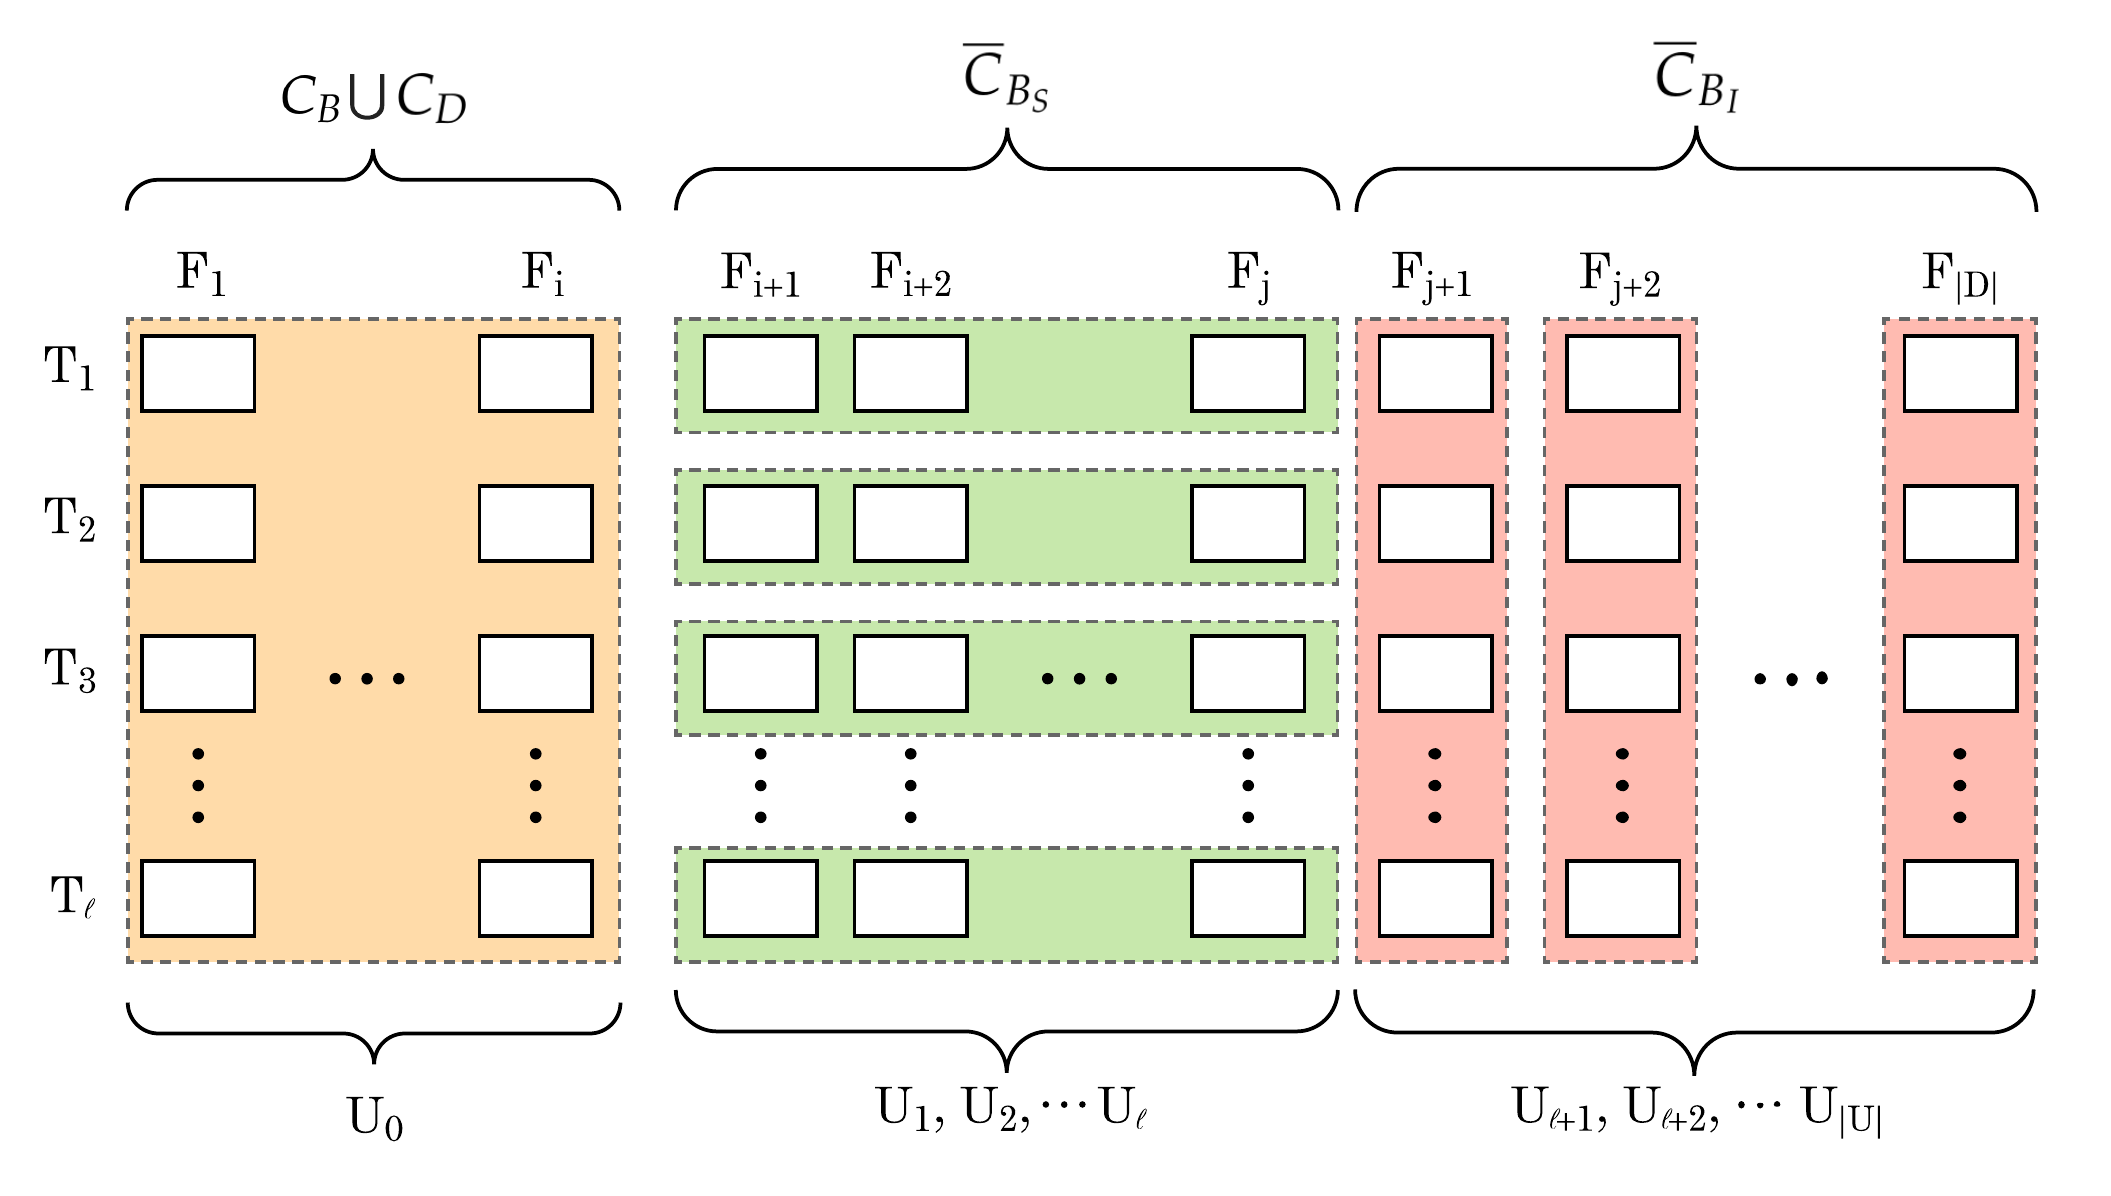
\includegraphics[origin=c,width=12cm]{../figures/sequence-dimensions.png}}
\caption{Dimensionality of Interval Values}
\label{fig:sequence_dimensions}
\end{figure}

The selected permutation value ($U_0$) is converted to a unique inversion sequence by again applying interval mapping. The inversion sequence is then used to construct the associated permutation using the technique introduced previously. The algorithm then produces level values by using each integer in the permutation as an index into the sequences in $X$.

The algorithm converts the selected values for independent basic factors ($U_{l+1}$ to $U_{|U|}$) similarly. Each selected value identifies a combination index, which the algorithm converts to a set of values using interval mapping. Each value is an index into the list of levels for the associated factor. % TODO - does this need more?

Lastly, the algorithm must convert the selected values for source combinations ($U_1$ to $U_l$). These are more complex than the previous conversions because a set of valid source combinations is associated with an individual trial in the sequence. It would be incorrect to select a source combination from the $n^{th}$ set of valid source combinations for the $n^{th}$ trial, because the permutation may have shifted the position of the original $n^{th}$ trial in the sequence. Therefore care must be taken to preserve this association. The algorithm preserves this association by using the original trial index when selecting the set of valid source combinations. Figure \ref{fig:source_combinations} outlines the entire mapping process.

% TODO: Make this a real diagram
\begin{figure}[htb]
\centering
\centerline{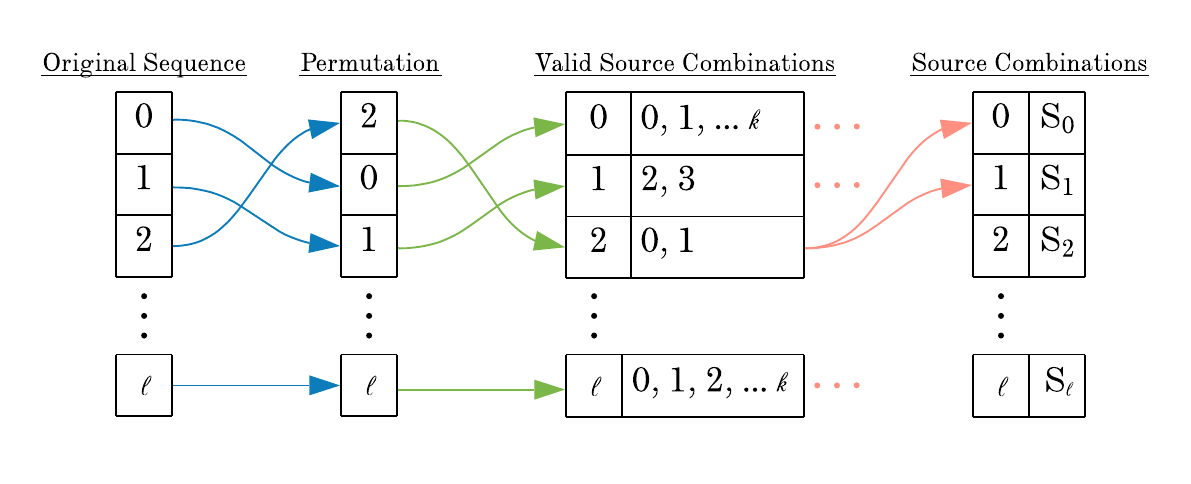
\includegraphics[origin=c,width=12cm]{../figures/source-combination-mapping.png}}
\caption{Selecting Valid Source Combinations}
\label{fig:source_combinations}
\end{figure}

For example, if the selected permutation places the original crossing value for trial number 2 in the zeroth position in the sequence (trial 0), then the source combination for trial 0 must also be selected from the valid source combinations originally generated for trial number 2.


\section{Example}

We will now use this method to construct a single solution to the design from the counting example in the previous chapter. We will choose a solution at random from $[1, 5760]$: $2590$.

First, we compute the set of value selections, $R$, for the $2,590^{th}$ solution. In order to do this, we first compute $U$, the set of upper-bounds for each range. The first upper bound is the number of permutations, $l!$, for the design. For this example, this was determined to be $720$. Next, we add the size of each subset of $S$ (See Table \ref{tab:example_s}) to $U$ to select valid source combinations. $U$ now contains 7 elements: $U = \{720, 1, 2, 1, 2, 1, 2\}$. Because $\overline{C}_{B_I} = \emptyset$ and $\overline{C}_D = \emptyset$ in this example, there are no other bounds to compute, so $U$ is complete.

When interval mapping is applied to $2590$ to generate values from these ranges, $R$ is determined to be $R = \{430, 0, 1, 0, 1, 0, 0\}$. With $R$ computed, we can now use the selected values to generate the correct permutation, and then select level combinations for the remaining factors.

To generate the $430^{th}$ permutation, we first construct the $430^{th}$ inversion sequence by again applying interval mapping with $U = \{6, 5, 4, 3, 2, 1\}$. This yields $\{4, 1, 2, 0, 1, 0\}$ as the $430^{th}$ inversion sequence. Applying the algorithm to convert this sequence to its corresponding permutation, we obtain $\{3, 1, 5, 2, 0, 4\}$. The crossing, $X$, was previously identified to be:

\begin{align*}
X = \{(red, yes), (red, no), (green, yes), (green, no), (blue, yes), (blue, no)\}
\end{align*}

The permutation $\{3, 1, 5, 2, 0, 4\}$ therefore corresponds to:

\[
    \{(green, no), (red, no), (blue, no), (green, yes), (red, yes), (blue, yes)\}
\]


We have now selected levels for factors in $C_B$ and $C_D$. The only remaining factor is \texttt{text}, which is in $\overline{C}_{B_S}$. The source combination selections from $R$ for this factor were $\{0, 1, 0, 1, 0, 0\}$. We then use the values from the permutation as indices to select both the source combination list and the selected value from that list for each trial. This process is represented visually in Figure \ref{fig:source_combinations}. We previously established the set of source combination lists as:

\[
S = \{(red), (green, blue), (green), (red, blue), (blue), (red, green)\}
\]

The first value of the permutation is $3$, which corresponds to the source combination list $(red, blue)$, and a value selection of $1$. Therefore the level selected for \texttt{text} in the first trial is $blue$. Following the same pattern, the level selections for \texttt{text} in each trial are:

\[
  \{blue, blue, red, green, red, blue\}
\]

Another perspective is that we are applying the same permutation computed previously to the list of level selections and the list of source combinations, before doing the final lookup. Combining all level selections yields a complete trial sequence:

\begin{table}[htb]
  \centering
  \caption{The $2590^{th}$ Trial Sequence}
\begin{tabular}{rccc}
\multicolumn{1}{c}{Trial} & Color   & Text    & Congruent \\ \hline
1                         & $green$ & $blue$  & $no$      \\
2                         & $red$   & $blue$  & $no$      \\
3                         & $blue$  & $red$   & $no$      \\
4                         & $green$ & $green$ & $yes$     \\
5                         & $red$   & $red$   & $yes$     \\
6                         & $blue$  & $blue$  & $yes$
\end{tabular}
\label{tab:example_trial_sequence}
\end{table}


% \begin{align*}
% i = 2,590 &&  R_1 = 2,590 \bmod 720 = 430 && i = \Bigl\lfloor \frac{2,590}{720} \Bigr\rfloor = 3 \\
% i = 3     &&  R_2 = 3 \bmod 1 = 0         && i = \Bigl\lfloor \frac{3}{1} \Bigr\rfloor = 3 \\
% i = 3     &&  R_3 = 3 \bmod 1 = 0         && i = \Bigl\lfloor \frac{3}{1} \Bigr\rfloor = 3 \\
% i = 3     &&  R_4 = 3 \bmod 1 = 0         && i = \Bigl\lfloor \frac{3}{1} \Bigr\rfloor = 3 \\
% i = 3     &&  R_5 = 3 \bmod 2 = 1         && i = \Bigl\lfloor \frac{3}{2} \Bigr\rfloor = 1 \\
% i = 1     &&  R_6 = 1 \bmod 2 = 1         && i = \Bigl\lfloor \frac{1}{2} \Bigr\rfloor = 0 \\
% i = 0     &&  R_7 = 0 \bmod 2 = 0         &&                                               \\
% \end{align*}

% To generate the $430^{th}$ permutation, we first construct the $430^{th}$ inversion sequence by applying interval mapping with $U = \{6, 5, 4, 3, 2, 1\}$:

% \begin{align*}
% i = 430  &&  R_1 = 430 \bmod 6 = 4  &&  i = \Bigl\lfloor \frac{430}{6} \Bigr\rfloor = 71 \\
% i = 71   &&  R_2 = 71 \bmod 5 = 1   &&  i = \Bigl\lfloor \frac{71}{5} \Bigr\rfloor = 14  \\
% i = 14   &&  R_3 = 14 \bmod 4 = 2   &&  i = \Bigl\lfloor \frac{14}{4} \Bigr\rfloor = 3   \\
% i = 3    &&  R_4 = 3 \bmod 3 = 0    &&  i = \Bigl\lfloor \frac{3}{3} \Bigr\rfloor = 1    \\
% i = 1    &&  R_5 = 1 \bmod 2 = 1    &&  i = \Bigl\lfloor \frac{1}{2} \Bigr\rfloor = 0    \\
% i = 0    &&  R_6 = 0 \bmod 1 = 0    &&                                                   \\
% \end{align*}




\section{Handling Constraints}

Recall that the complexity gradation did not account for the external constraints that may be part of the design. Such constraints typically enforce some rule regarding repetition of particular characteristics. For example, in the design for Stroop experiments, it is common to apply a constraint that requires that the generated sequence never contain two consecutive congruent trials. Constraints may be applied to the levels of derived factors as well; therefore, the user may impose practically any condition upon the generated sequence.

In the future, the counting and construction algorithms could be enhanced to account for these constraints. Such improvements will be discussed further later on. In the meantime, however, rejection sampling is applied to ensure that the algorithm does not ever return sequences that violate constraints. The generated sample is checked against all repetition constraints in the design to verify that no violations exist. As will be seen in the next section, this performs adequately in practice.


\section{Benchmarks}

Of the ten benchmarks designs that were introduced previously, four can be classified as tier 1, 2, or 3 designs: \texttt{stroop-2}, \texttt{stroop-3}, \texttt{stroop-4}, \texttt{stroop-5}. We will repeat the benchmarks for those designs here using this construction approach to sampling. We will also introduce a few additional designs involving variations on the Stroop design to demonstrate the scalability of this approach and the empirical performance of the rejection sampling phase. Table \ref{tab:benchmark_experiments_construction} reviews the basic experiment data for each benchmark design. Table \ref{tab:sampling_metrics} summarizes the time required to generate 10,000 samples for each design using a single core, as well as the average number of rejections per sample. (Rejections caused by constructing a trial sequence that violated external constraints.)

% Extra constraints:
% constraints = [AtMostKInARow(1, ("congruent?", "yes")), AtMostKInARow(3, color), AtMostKInARow(3, text)]

\begin{table}[htb]
  \centering
  \caption{Benchmark Experiments for Sequence Construction}
\begin{tabular}{|c|c|c|c|c|}
\hline
\multicolumn{1}{|l|}{Experiment Name} & Length          & Unconstrained Solutions  & Single Sample  \\ \hline
stroop-2                              & 4               & 24                       & 0.0009s        \\ \hline
stroop-3                              & 9               & 362,880                  & 0.003s         \\ \hline
stroop-4                              & 16              & 20,922,789,888,000       & 0.007s         \\ \hline
stroop-5                              & 25              & $\approx 2^{83}$         & 0.016s         \\ \hline
stroop-10                             & 100             & $\approx 2^{524}$        & 0.170s         \\ \hline
stroop-20                             & 400             & $\approx 2^{2886}$       & 2.729s         \\ \hline
stroop-20-extra-constraints           & 400             & $\approx 2^{2886}$       & 3.234s         \\ \hline
\end{tabular}
\label{tab:benchmark_experiments_construction}
\end{table}

Even for huge designs, this approach constructs a single random sample exceptionally quickly.

\begin{table}[htb]
  \centering
  \caption{Sampling Metrics}
\begin{tabular}{|c|c|c|c|c|}
\hline
\multicolumn{1}{|l|}{Experiment Name} & 10,000 Samples & Avg. Rejections/Sample  \\ \hline
stroop-2                              & 8.763s         & 0.982                   \\ \hline
stroop-3                              & 29.323s        & 1.393                   \\ \hline
stroop-4                              & 72.882s        & 1.53
8                   \\ \hline
stroop-5                              & 155.699s       & 1.589                   \\ \hline
stroop-10                             & 1908.598s      & 1.698                   \\ \hline
stroop-20                             & 26064.417s     & 1.684                   \\ \hline
stroop-20-extra-constraints           & 27338.002s     & 1.898                   \\ \hline
\end{tabular}
\label{tab:sampling_metrics}
\end{table}

Generating a large number of samples can still take a significant amount of time. However, because samples can be generated independently of one another, this algorithm can be easily parallelized for a linear speedup in the number of available cores.

%%% -*-LaTeX-*-

\chapter{Future Work}

This paper has presented an approach for constructing trial sequences for some experimental designs based on a bijection between the natural numbers and viable trial sequences. This approach is beneficial in that sampled sequences are guaranteed to be uniformly distributed, and sequences can be constructed nearly instantaneously. This is a vast improvement over  the prior approach of sampling solutions using SAT Sampling. However, there are many ways in which it could be improved and other alternatives that should be researched.

The counting and construction methods presented here apply to several tiers of experimental designs, yet they do not account for external constraints that may be specified as part of the design. They only ensure that no internal constraints (between basic and derived factors) are violated and rely on rejection sampling to discard generated samples that violate external contraints. While rejecting sampling is sufficient in practice for many designs, it is possible to construct designs with external constraints that would make the solution space so sparse as to render rejection sampling impractical. Further research to incorporate constraints in the counting and construction process would be worthwhile. Combinatoric techniques for generating permutations with prohibited patterns would be likely be applicable to this process.

Additionally, the existing methods cannot yet construct sequences for designs beyond tier 3 which include derived factors spanning multiple trials. (Derived factors with complex windows.) The approaches presented here could reasonably be extended to apply to tier 4 designs (which allow \texttt{Transition} windows) with small adjustments. Increasing their capability to handle tier 5 designs would also be worthwhile, though significantly more difficult due to potential overlap and staggering between different derived factors. It is likely that rejection sampling could continue to handle constraints even for these advanced designs, if the construction methods could be discovered.

As an implementation detail, the current construction algorithm is single threaded, requiring all samples to be generated serially. However there is no dependent relationship between samples, therefore the construction algorithm can be fully parallelized for a linear speedup in the number of available cores.

There are other approaches that could also be considered which do not rely wholly upon direct construction. Various hybrid approaches have been considered, but not thoroughly researched. As an example, a numeric construction approach could be used to construct a partial trial sequence which could then be completed using a SAT sampler, once the solution space had been sufficiently reduced. This would more efficient sample generation for all designs, but care would need to be taken to preserve uniformity guarantees. It is possible that a partially constructed sequence may overprune the remaning search space, leading to biased results.

Lastly, the SAT encoding itself may be altered. The naive encoding used currently is easy to understand and reason about, but is wasteful in its representation. Far more variables are used then are theoretically required to represent the data. If other types of encoding schemes were researched, an alternative may be discovered that could improve performance. Such an encoding would still likely need to avoid encoding all permutations as distinct solutions to avoid a combinatoric explosion. A hybrid approach, the inverse of the previous paragraph, would likely perform well so long as the size of the independent support set were kept small: A SAT encoding could be developed to partially construct a sequence, including sampling the most complex aspects such as derived factors and constraints, while the remaining simpler values could be populated using a construction approach. This would reduce the burden on the SAT tooling and potentially simplify the construction algorithm. In the same vein, SweetPea could also begin utilizing the native \texttt{XOR} support offered by CryptoMiniSat, which may also offer performance improvements.

%%% -*-LaTeX-*-

\chapter{Conclusion}

The current implementation of SweetPea provides a useful standard language for defining experimental designs. However, it has not yet fully achieved its objective to generate uniformly-distributed trial sequences conforming to these designs. This failure is due primarily to the inability of current SAT sampling tools to cope with such large and complex solution spaces. While SAT tools are still useful for quickly generating solutions to in-progress designs, SweetPea has not yet been successful in guaranteeing uniformly-distributed samples for arbitrary designs using these tools.

This thesis has presented background information and benchmarks detailing these shortcomings and has introduced a complexity gradation for discussing experimental designs of varying complexity. It also introduced methods for enumerating arbitrary solutions to tier one, two, and three designs. These methods allow efficient generation of samples which are guaranteed to follow a uniform distribution for these design tiers. As these techniques do not yet account for external design constraints, rejection sampling is applied to ensure that no generated sequences violate these constraints.

While not yet able to achieve SweetPea's objectives for all experimental designs, this approach is hugely beneficial for simple designs. Uniformly-distributed samples can be generated exceptionally quickly, and have the added benefit of being numbered. It also provides a framework and pattern upon which to build for more complicated designs. We expect that these methods can be extended or hybridized to guarantee uniformly distributed samples to all experimental designs.


% \numberofappendices = 1   % Set 0 for none, else number of appendices.
% \numberofappendices = 3
% \appendix       % Chapters, sections are now appendix style A, A.1, A.2, B, C, D, ...

% \include {appa}
% \include {appb}
% \include {appc}

%%% The choice of bibliography style is a major decision, jointly made
%%% by you, your thesis advisor and the thesis editor. Common choices are
%%% one of the four standard BibTeX styles (abbrv, alpha, plain, and unsrt),
%%% or enhanced styles like acm, amsplain, siam, and hundreds of others
%%% available in TeX Live, and other Unix and Windows TeX distributions.
%%%
%%% Do NOT handcode your reference list, because you are unlikely to
%%% achieve consistency or conformance to the University of Utah Thesis Office
%%% requirements: let BibTeX do that tedious job for you!
%%%
%%% Remember that reference-list metadata in BibTeX files remains
%%% constant across journals and publishers, and is are often reused
%%% in other documents and shared with others, whereas formatted
%%% reference-list styles change: with BibTeX, you only need to record
%%% the metadata once.
%%%
%%% If you prefer named, rather than numeric or tagged citations, you
%%% may use styles such as authordate{1,2,3,4}, chicago, harvard, or
%%% natbib.  Be aware, however, that most of those require an
%%% additional \usepackage{} command to supply \LaTeX{} with
%%% definitions of commands that the style needs, and that there are
%%% usually several flavors of LaTeX citation commands beyond the
%%% standard \cite{} command that you need to understand before you
%%% can use them properly in your prose.

%%% This tells BibTeX to read siam.bst from the first directory where
%%% it is found in the BSTINPUTS search path:

\bibliographystyle{siam}

%%% This can also specify a comma-separated list (without embedded
%%% spaces) of *.bib files found by BibTeX in its BIBINPUTS search
%%% path.  The argument \jobname means the base name of the top-level
%%% LaTeX file, avoiding an unnecessary filename dependence here.
%%%
%%% BibTeX writes only one .bbl file, no matter how many *.bib files
%%% are listed here, using the name \jobname.bbl.
%%%
%%% LaTeX reads BibTeX's formatted reference list from the file
%%% \jobname.bbl.

\bibliography{\jobname}

\end {document}
